\documentclass[conference]{IEEEtran}
\IEEEoverridecommandlockouts
% The preceding line is only needed to identify funding in the first footnote. If that is unneeded, please comment it out.
\usepackage{cite}
\ifCLASSOPTIONcompsoc \usepackage[caption=false,font=normalsize,labelfon
t=sf,textfont=sf]{subfig}
\else
\usepackage[caption=false,font=footnotesize]{subfi g}
\fi
\usepackage{amsmath,amssymb,amsfonts}
\usepackage{algorithmic}
\usepackage{graphicx}
\usepackage{textcomp}
\usepackage{xcolor}
\def\BibTeX{{\rm B\kern-.05em{\sc i\kern-.025em b}\kern-.08em
    T\kern-.1667em\lower.7ex\hbox{E}\kern-.125emX}}
\begin{document}

\title{Linear Quadratic Integral Differential Game applied to the Real-time Control of a 3DoF Experimental setup of a Quadrotor\\
% {\footnotesize \textsuperscript{*}Note: Sub-titles are not captured in Xplore and
% should not be used}
% \thanks{In partnership with BaniAsad Industries}
}

\author{\IEEEauthorblockN{Hadi Nobahari}
\IEEEauthorblockA{\textit{Department of Aerospace Engineering} \\
\textit{Sharif University of Technology}\\
Tehran, Iran \\
nobahari@sharif.edu}
\and
\IEEEauthorblockN{Ali BaniAsad}
\IEEEauthorblockA{\textit{Department of Aerospace Engineering} \\
\textit{Sharif University of Technology}\\
Tehran, Iran \\
ali.baniasad@ae.sharif.edu}
\and
\IEEEauthorblockN{Alireza Sharifi}
\IEEEauthorblockA{\textit{Department of Aerospace Engineering} \\
\textit{Sharif University of Technology}\\
Tehran, Iran \\
alireza\_sharifi@ae.sharif.edu}
% \and
% \IEEEauthorblockN{Alireza Sharifi}
% \IEEEauthorblockA{\textit{Department of Aerospace Engineering} \\
% \textit{Sharif University of Technology}\\
% Tehran, Iran \\
% alireza_sharifi@ae.sharif.edu}



% \and
% \IEEEauthorblockN{3\textsuperscript{rd} Given Name Surname}
% \IEEEauthorblockA{\textit{dept. name of organization (of Aff.)} \\
% \textit{name of organization (of Aff.)}\\
% City, Country \\
% email address or ORCID}
% \and
% \IEEEauthorblockN{4\textsuperscript{th} Given Name Surname}
% \IEEEauthorblockA{\textit{dept. name of organization (of Aff.)} \\
% \textit{name of organization (of Aff.)}\\
% City, Country \\
% email address or ORCID}
% \and
% \IEEEauthorblockN{5\textsuperscript{th} Given Name Surname}
% \IEEEauthorblockA{\textit{dept. name of organization (of Aff.)} \\
% \textit{name of organization (of Aff.)}\\
% City, Country \\
% email address or ORCID}
% \and
% \IEEEauthorblockN{6\textsuperscript{th} Given Name Surname}
% \IEEEauthorblockA{\textit{dept. name of organization (of Aff.)} \\
% \textit{name of organization (of Aff.)}\\
% City, Country \\
% email address or ORCID}
}

\maketitle

\begin{abstract}
    % In this paper, a quadcopter stand with three degrees of freedom was controlled using game theory-based control. The first player tracks the desired input, and the second player creates a disturbance in the tracking of the first player to cause an error in the tracking. The control effort is chosen using the Nash equilibrium, which presupposes that the other player made the worst move. In addition to being resistant to input interruptions, this method may also be resilient to modeling system uncertainty. This method evaluated the performance through simulation in the Simulink environment and implementation on a three-degree-of-freedom stand.
	% In this study, a linear quadratic with integral action based on the differential game theory is implemented real-time for a three-degree-of-freedom experimental setup of a quadrotor. For this purpose, two players are considered for each of roll, pitch, and yaw channels of the quadrotor.
	% First player searches the best control command for each channels of the setup of a quadrotor based on the minimization a quadratic criterion; when the worst disturbances are produced by the second player. Performance of the proposed controller is evaluated in level flight and compared to the LQR controller.
	The accurate attitude control of a quadrotor is necessary, especially when facing disturbance. In this study, a linear quadratic with integral action based on the differential game theory is implemented on a three-degree-of-freedom experimental setup of a quadrotor. For this purpose, first, a continuous state-space model of the quadrotor is derived based on the linearization of the nonlinear equations of motion, and the parameters of the state-space model structure are identified with the experimental results. Then, the attitude control commands of the quadrotor are derived based on two players; one finds the best attitude control command, and the other creates the disturbance by minimizing a quadratic criterion, defined as the sum of outputs plus the weighted control effort. The performance of the proposed controller is evaluated in level flight and compared to the linear quadratic regulator controller. Results demonstrate that the proposed approach has an excellent performance in dissipating the disturbances created by the modeling error.
\end{abstract}

\begin{IEEEkeywords}
    Linear Quadratic Differential Game, Quadrotor, Real-time, 3DoF Experimental setup, Optimal Control, Robust Control
\end{IEEEkeywords}

\section{Introduction}
% % This document is a model and instructions for \LaTeX.
% % Please observe the conference page limits. 
% A quadcopter is a type of helicopter with four rotors. % https://en.wikipedia.org/wiki/Quadcopter#cite_note-dasc04-1
% Quadcopters have extensive applications due to their excellent maneuverability and the possibility of hover flight with high balance.
% % The outstanding maneuverability of quadcopters and the possibility of hover flight with a high balance make them very useful.
% In recent years, companies, universities, and research centers have attracted more to this type of UAV.
% % Many companies, universities, and research centers have recently become interested in these UAVs.
% % It has become increasingly popular for companies, universities, and research centers to use this type of UAV in recent years.
% In this way, the facilities and the flight of these UAVs are continuously improving.
% % These UAVs are undergoing significant improvements in facilities and performance each day.
% % This leads to significant improvements in the facilities and flight of these UAVs daily.
% Quadcopters are widely used in research, military, imaging, recreation, and agriculture.
% % In agriculture, research, military, imaging, and recreation, quadcopters are widely used
% % Researchers, military, imagers, recreation, and farmers use quadcopters in various applications.
% Mathematical models are used in game theory to examine how rational, intelligent beings cooperate or compete.
% % Game theory uses mathematical models to analyze the cooperation or competition methods of logical and intelligent beings.
% Game theory can be applied to pursuit and evasion as one of its broad
% applications.
% % One of the broad applications of game theory is pursuit-evasion
% There can be two \cite{b1} or more players \cite{b2} involved in the pursuit-evasion.
% Pursuit-evasion can occur indoors as well \cite{b3}.
% % Two or more players can participate in the pursuit-evasion.
% In some cases, machine learning and differential games pursuit-evade \cite{b4}.
% Players may play different roles in differential games, such as protecting some targets \cite{b5}.
% % The players in a differential game may have a different roles, such as protecting a specific target.
% % Differential games may have different roles for the players, for example, protecting some targets.
% % There may be a different role for each player in a differential game, for example, the role of protecting a specific target.
% The differential game's ability to examine the actions of two or more players makes it powerful.
% % The power of the differential game is to analyze the behavior of two or more players.
% Player cooperation can be used through swarm platooning \cite{b6}.
% Multi-agent \cite{b7} and self-driving automobiles \cite{b8} motion planning are two other applications of player cooperation.
% % Autonomous cars and multi-agent motion planning are two other applications of player cooperation.


% Due to the widespread use of quadrotors, their control has become an important issue.
% % Quadrotor control has become increasingly important as they are widely used.
% In order to control quadrotors, neural networks \cite{b9} and machine learning \cite{b10} methods have been used.
% % Neural networks and machine learning methods have been used to control quadrotors.
% % For quadrotor control, neural networks and machine learning techniques have been used.
% Two uses for quadrotor control include swarm flying \cite{b12} and motion planning \cite{b11}.
% % Swarm flight and motion planning are two applications of quadrotor control.
% In \cite{b13}, Kyuman Lee, Daegyun Choi, and Donghoon Kim worked on  Motion Planning for Quadcopters in Three-Dimensional Dynamic Environments with Potential Fields-Aided.
% To avoid collisions with obstacles, the controller should control the quadrotor to prevent collisions \cite{b14}.

A quadrotor is a type of helicopter with four rotors that plays a significant role in today's society, including research, military, imaging, recreation, and agriculture. The performance of the quadrotor relies on the control system, including attitude, altitude, and position subsystems. In the attitude control of the quadrotor, it is necessary to maintain the attitude outputs, including roll, pitch, and yaw angles of the quadrotor, at the desired level using control commands such as the rotational speed of the rotors, mainly when the disturbances occur suddenly. Therefore, much research is being conducted on the automatic control of the attitudes' quadrotor in facing the disturbance.
     In \cite{PID}, a Proportional Integral Derivative (PID) controller is used to control the attitude of the quadrotor. However, the control objectives have not been effectively achieved with this controllers category due to the nonlinearity of quadrotor dynamics, primarily when the disturbance occurs. The model-based approaches \cite{model_base} for controller design are needed to solve these problems. These controllers work based on information from the dynamic attitude model of the quadrotor and the disturbance to produce the best control command.
     Various model-based controllers can be found within the literature, the most well-known of which are intelligent control, nonlinear control, robust control, and optimal control to reduce the disturbance effect in the attitude control and provide a faster control algorithm in facing the modeling error. In the intelligent controller category, artificial intelligence computing approaches like fuzzy logic \cite{fuzzy}, iterative learning \cite{iterative_Learning}, machine learning \cite{machine_learning}, reinforcement learning \cite{Reinforcement_Learning}, and evolutionary computation \cite{Evolutionary} have been utilized to control the attitude of the quadrotor.
     Moreover, nonlinear control methods such as Sliding Mode Control (SMC) \cite{SMC} and Feedback Linearization (FBL) \cite{FBL} have been applied to control the roll, pitch, and yaw angles of the quadrotor. In the optimal controller category, a Linear Quadratic Regulator (LQR) \cite{LQR} and Linear Quadratic Gaussian (LQG) \cite{LQG} have been implemented on the wind turbine model based on the minimization of a quadratic criterion, including regulation performance and control effort to provide optimally controlled feedback gains. 
     LQDG control approach \cite{LQDG} is a class of optimal and robust controller methods that controls the outputs of a system based on its linear model and minimization of a cost function. This approach has been utilized to stabilize and control various nonlinear and complex systems such as a robust ship controller design \cite{LQDG_ship}, a min-max robust controller \cite{robust_LQDG}. Moreover, in the LQR-DG control method, the control commands are analytically generated based on a pursuit-evasion of two players, one tracks the best attitude control command, and the other creates the disturbance. This is one of the distinctive features of the LQR-DG controller and an important difference from other optimal control methods.
     In this study, an LQIR method based on the differential game theory, called LQIR-DG, is proposed to generate the most efficient control command for an experimental setup of the quadrotor when facing the disturbance. Since the LQIR-DG is affected by an accurate model of the system, first, the dynamic of the three-degree-of-freedom setup of a quadrotor is modeled. Then, the linear state-space form of the wind turbine tower model is extracted using the linearization of the nonlinear equations of motion to utilize in the predictive control problem. Moreover, the model's parameters are identified and verified against the experimental values. Next, the LQIR-DG technique is applied to the experimental setup of the quadrotor to reduce the effect of disturbance. The performance of the proposed controller is examined in the presence of the disturbance, including the modeling error. The results show the successful performance of the LQIR-DG scheme in reducing the disturbance.
     This paper is organized as follows: The problem architecture is defined in section \ref{sec:problem_statement}. In section \ref{sec:modeling}, the dynamics model for the experimental setup of the quadrotor is derived in detail. In section \ref{sec: diff game}, The LQIR-DG architecture is denoted. Numerical results are provided in section \ref{sec:results}. Finally, a conclusion is made in section \ref{sec:conclusion}.






\section{Problem Statement}\label{sec:problem_statement}
% First, this section presents a nonlinear dynamic model of the three degrees of freedom quadrotor, \figurename{\ref{quadlab}}, for control purposes.
In this section, a nonlinear dynamic is presented for an experimental setup of a quadrotor, as shown in \figurename{\ref{quadlab}}.
The quadrotor is free to rotate about its roll, pitch, and yaw axes. The Euler angle angles and angular velocities along three orthogonal axes are measured simultaneously using Attitude and Heading Reference Systems (AHRS). LQDG utilizes these noisy measurements for real-time control of the Euler angles. The block diagram of the control purpose is shown in \figurename{\ref{block_diagram}}.
\begin{figure}[!h]
	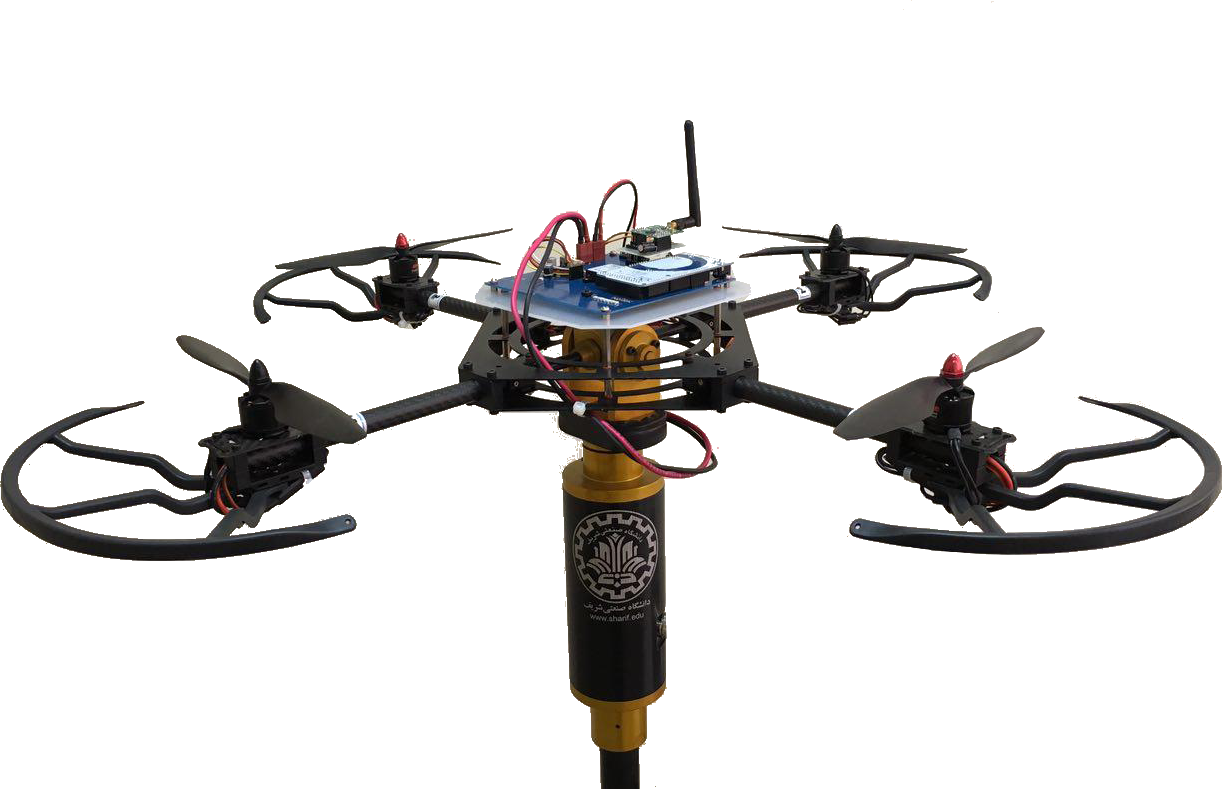
\includegraphics[width=6cm]{../Figures/introduction/3DOFQuad.png}
	\centering
	\caption{3DoF experimental setup of a quadrotor}
	\label{quadlab}
\end{figure}
\begin{figure}[!h]
	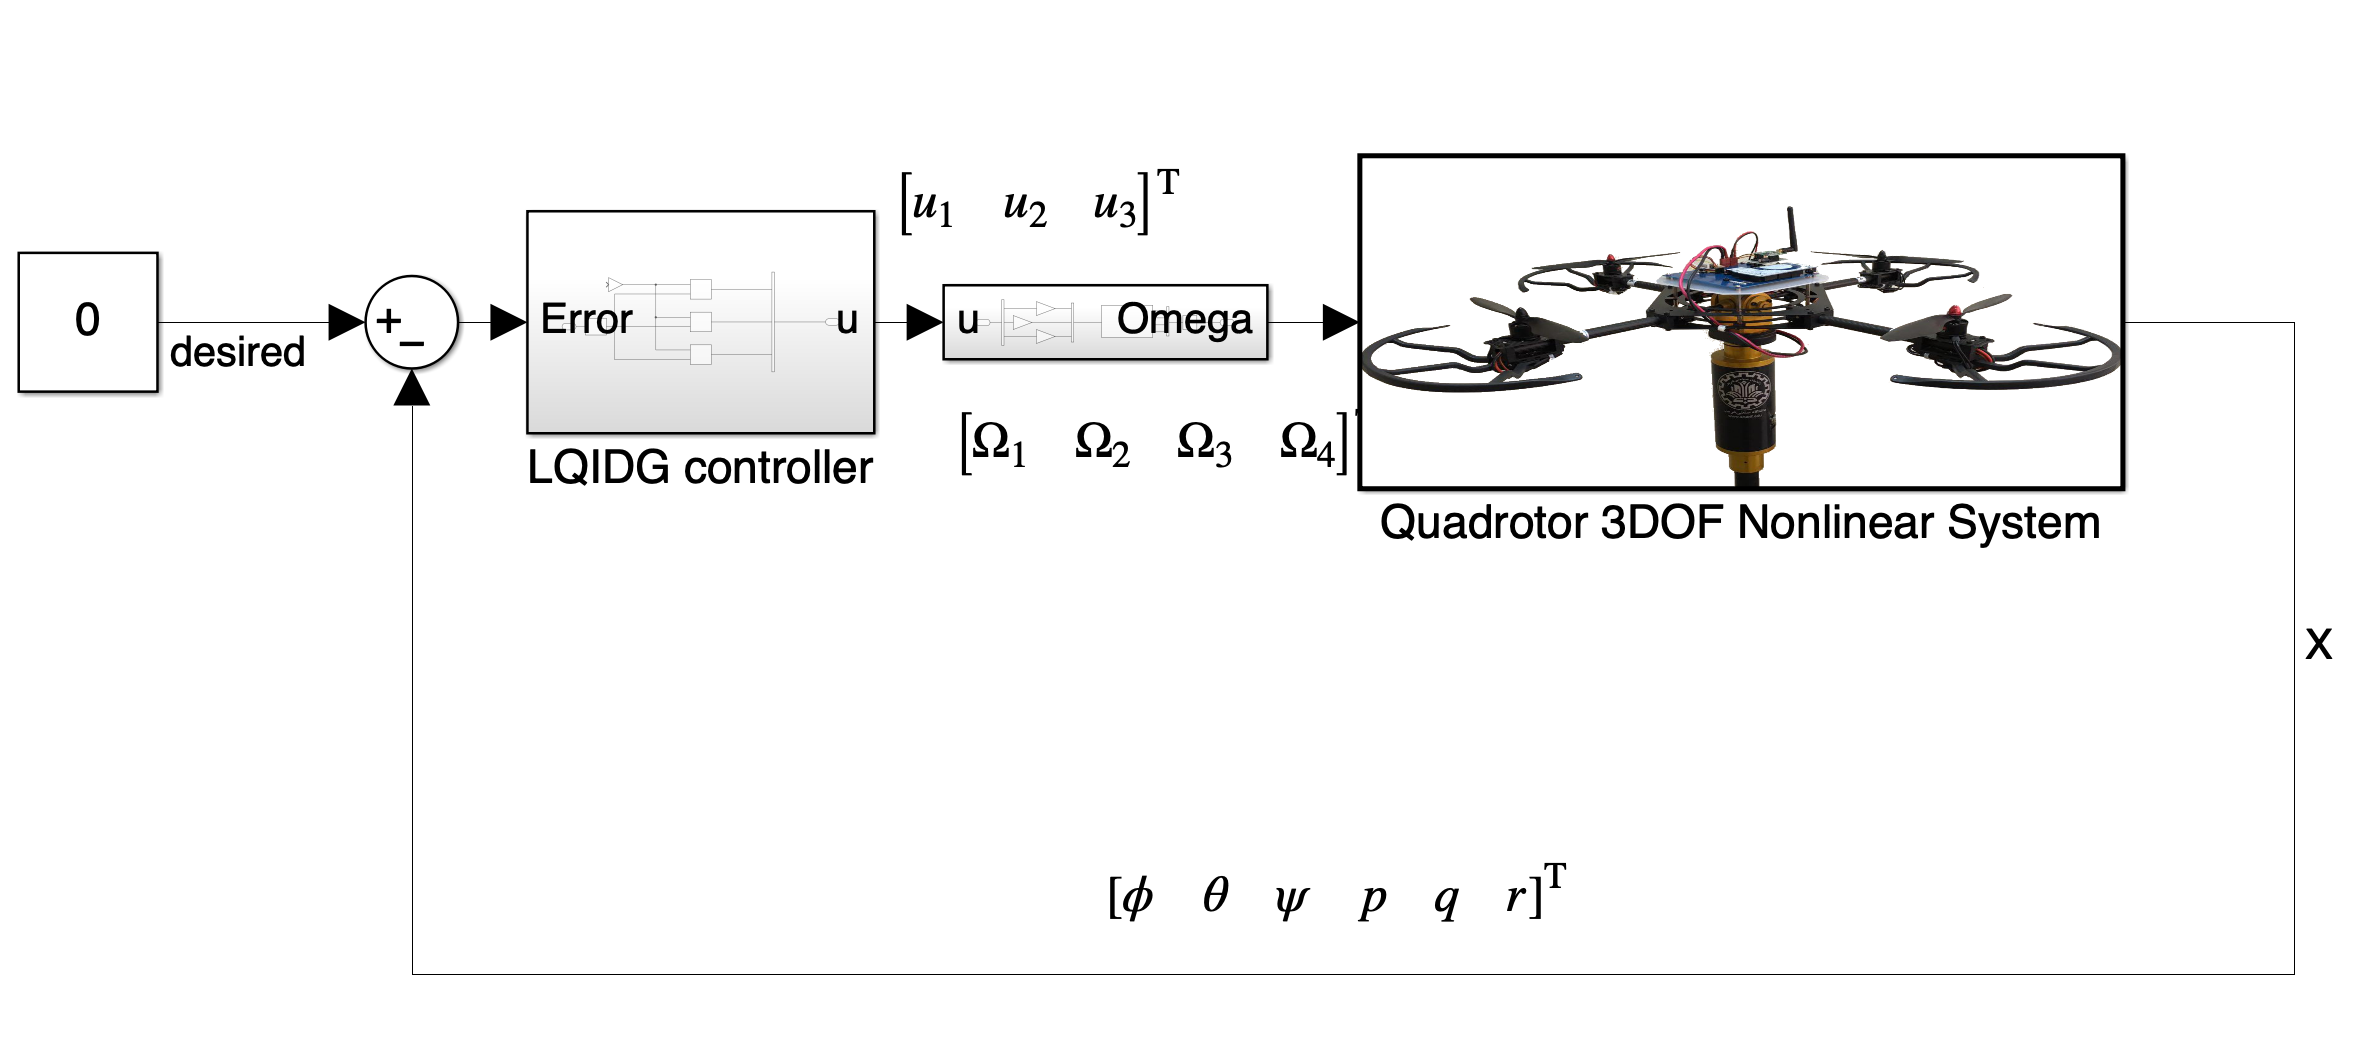
\includegraphics[width=.9\linewidth]{../Figures/introduction/block_diagram.png}
	\centering
	\caption{block diagram of the control purpose}
	\label{block_diagram}
\end{figure}


\section{Modeling of an Experimental Setup of a Quadrotor}\label{sec:modeling}
\subsection{Configuration of the Quadrotor }
The schematic of a quadrotor is given in \figurename{\ref{QuadAssum}}. Each rotor is considered a rigid disk is rotating about the axis $Z_B$ in the body fixed frame with an angular velocity $\Omega_i$.
Rotors 1 and 3 rotate in the same direction, i.e., counterclockwise, while rotors 2 and 4 rotate in the opposite direction, i.e., clockwise, to cancel yawing moment of the quadrotor.
\begin{figure}[!h]
	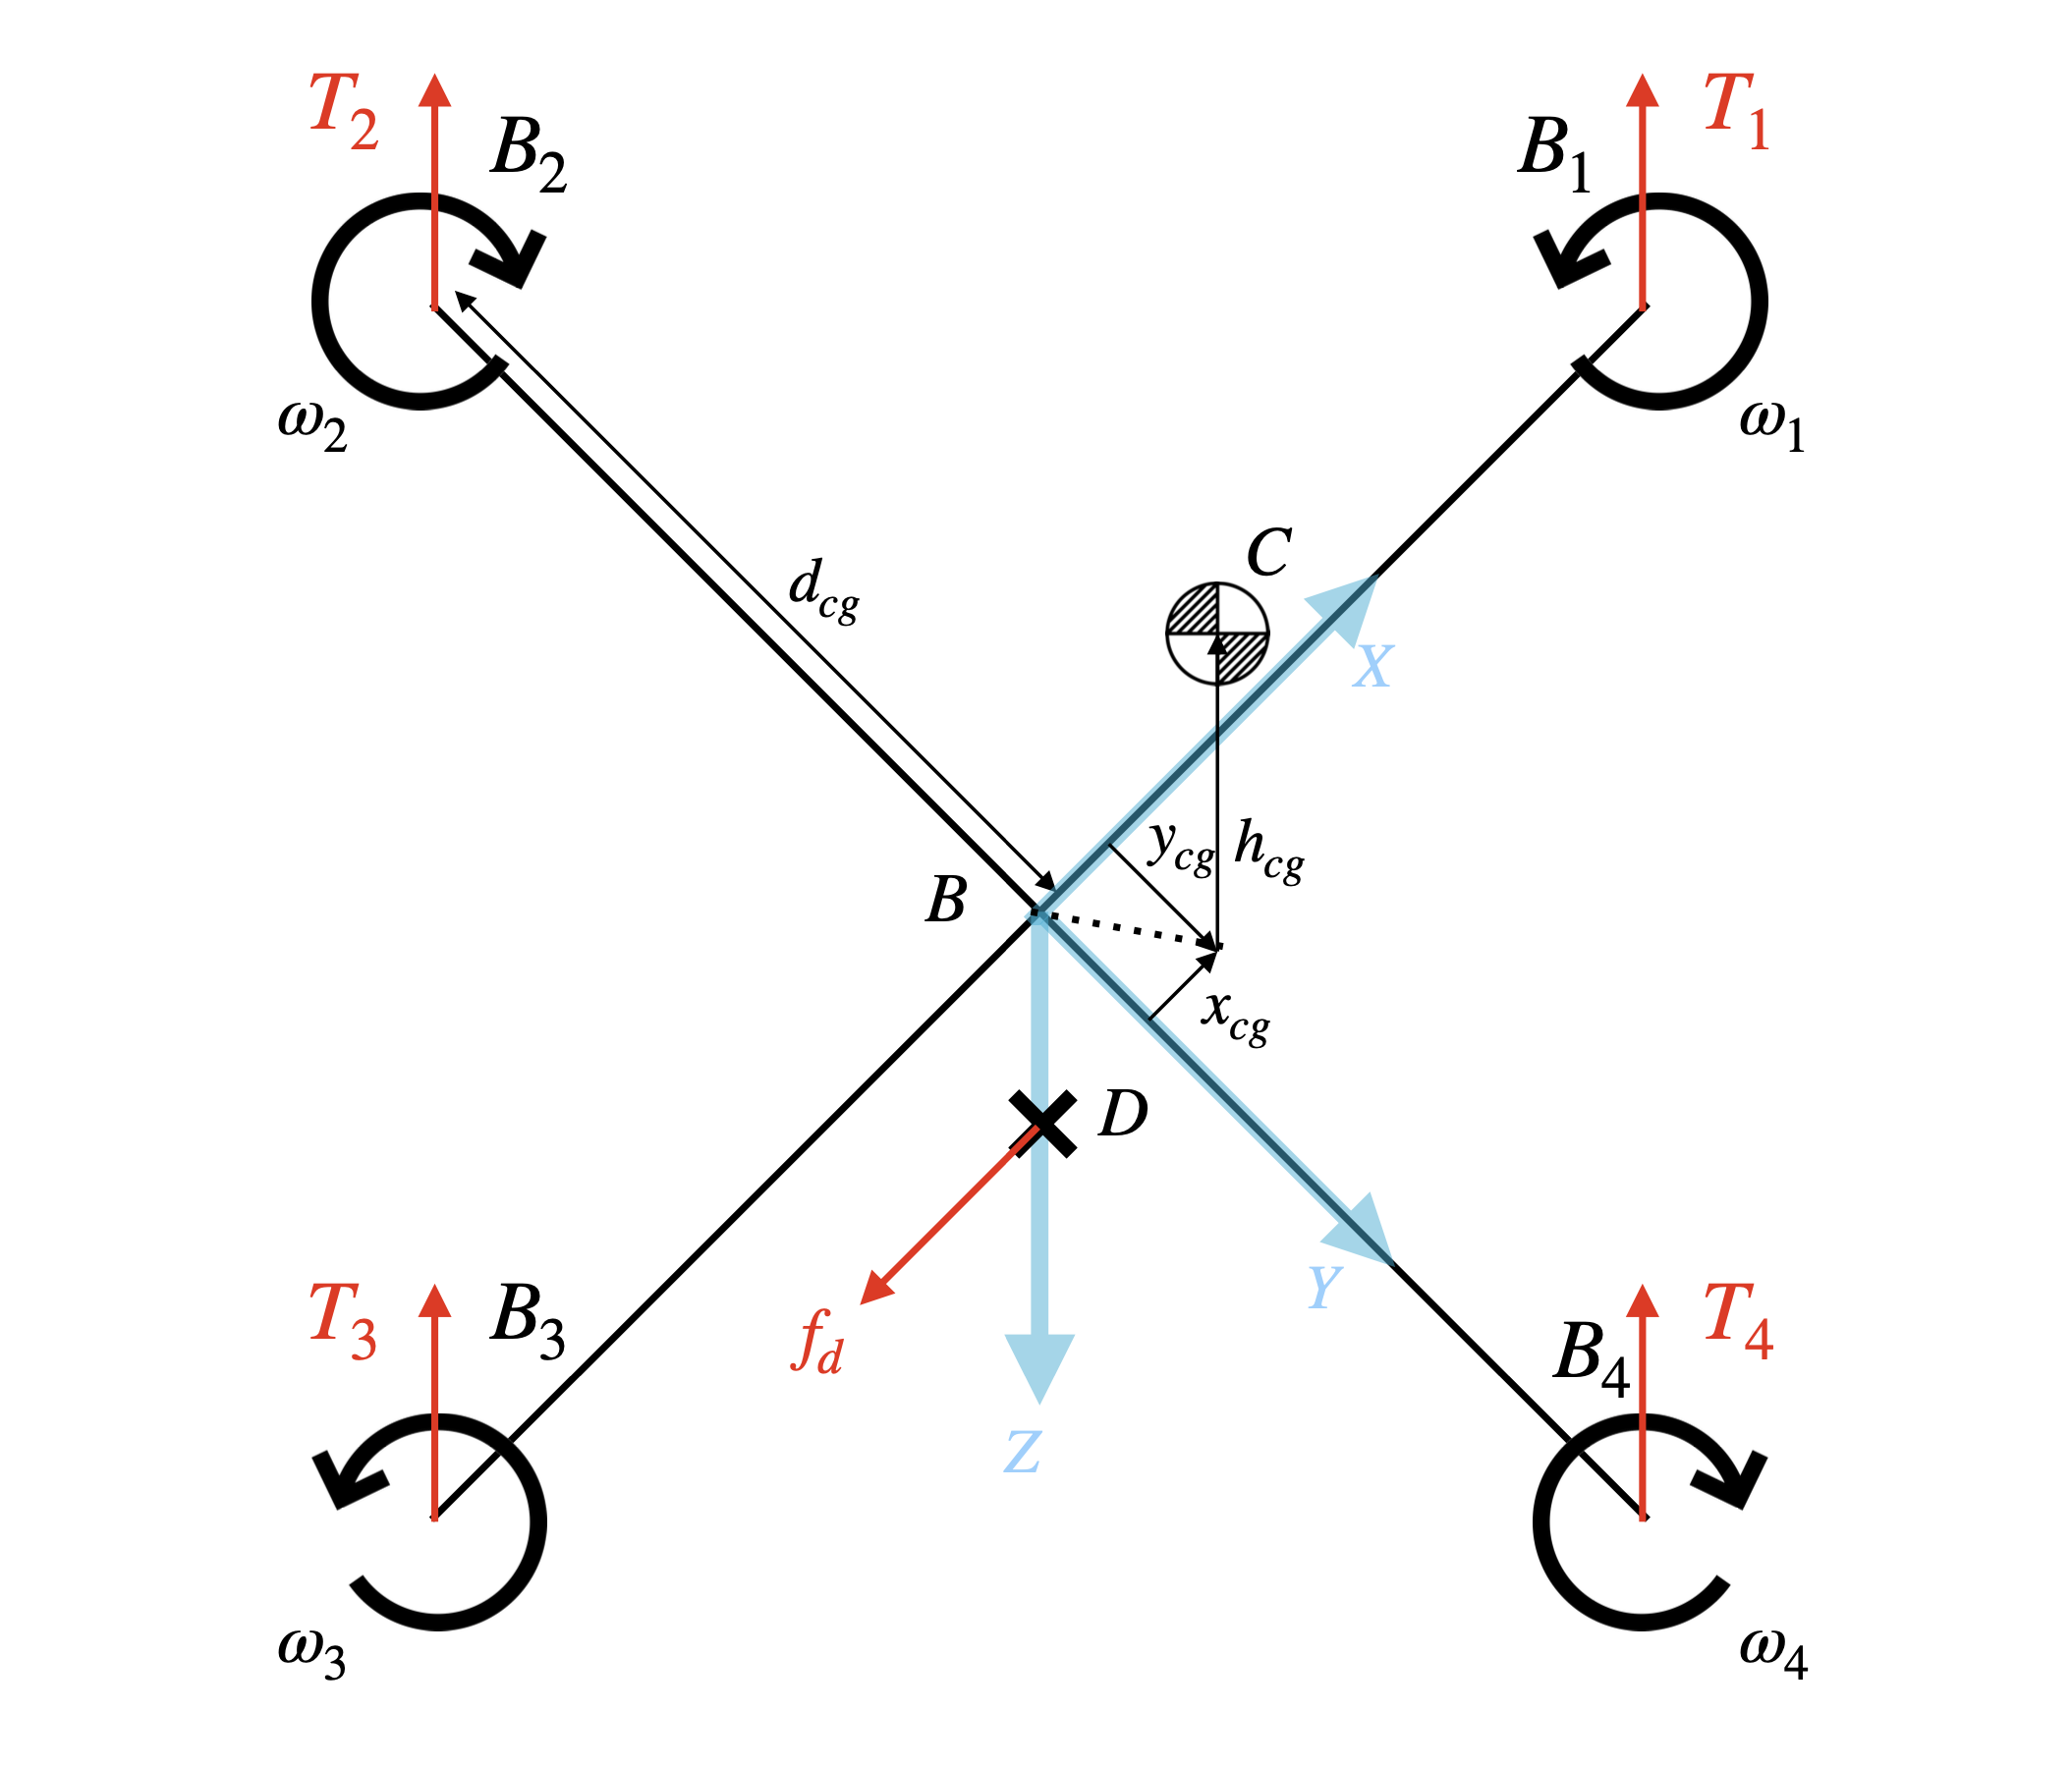
\includegraphics[width=6cm]{../Figures/Forces/StandAssumations.png}
	\centering
	\caption{Configuration of the quadrotor}
	\label{QuadAssum}
\end{figure}
\subsection{Dynamic Model}
The dynamic model of the quadrotor, obtained from the Newton-Euler method, is stated as follows \cite{b15}, \cite{b16}:
\begin{equation}
	\begin{split}
		&\dot p = \dfrac{I_{yy} - I_{zz}}{I_{\text{xx}}} qr + q \dfrac{I_{\text{rotor}}}{I_{\text{xx}}}\Omega_r + \dfrac{u_{\text{roll}}}{I_{\text{xx}}} + \dfrac{d_{\text{roll}}}{I_{\text{xx}}} \\
		&\dot q = \dfrac{I_{zz} - I_{zz}}{I_{yy}} rp + p \dfrac{I_{\text{rotor}}}{I_{\text{xx}}}\Omega_r + \dfrac{u_{\text{pitch}}}{I_{yy}} + \dfrac{d_{\text{pitch}}}{I_{yy}} \\
		&\dot r = \dfrac{I_{\text{xx}} - I_{yy}}{I_{zz}} pq  +  \dfrac{u_{\text{yaw}}}{I_{zz}} + \dfrac{d_{\text{yaw}}}{I_{zz}}
	\end{split}
\end{equation}
where $d_{\text{roll}}$, $d_{\text{pitch}}$, and $d_{\text{yaw}}$ are roll, pitch, and yaw moments, generated by the disturbance and  $(p, q, r)$ are the angular velocities, and $(\phi, \theta, \psi)$ are roll, pitch, and yaw angles. The relation between Euler angles rates and the angular body rates are obtained as follows:

\begin{equation}
	\begin{split}
		\dot\phi &= p + q\sin(\phi)\cos(\theta) + r\cos(\phi)\tan(\theta)\\
		\dot \theta &= q\cos(\phi) - r\sin(\phi)\\
		\dot\psi &= (q\sin(phi) + r\cos(\phi))\sec(\theta) 
	\end{split}
\end{equation}
where $I_{\text{xx}}$, $I_{yy}$, and $I_{zz}$ are the principal moment of inertia and $I_{\text{rotor}}$ is the inertia of a rotor about its axis. Moreover, $\Omega_r$, called the overall residual propeller angular speed, is computed as:
\begin{equation}
	\Omega_r = -\omega_1 + \omega_2 - \omega_3 + \omega_4
\end{equation}
The control inputs $u_{\text{roll}}$, $u_{\text{pitch}}$, and $u_{\text{yaw}}$ are roll, pitch, and yaw moments, generated by the propellers, defined as:
\begin{equation}
	\begin{split}
		u_{\text{roll}} &= bd_{cg} (\Omega_2^2 - \Omega_4^2) \\
		u_{\text{pitch}} &= bd_{cg} (\Omega_1^2 - \Omega_3^2) \\
		u_{\text{yaw}} &= d (\Omega_1^2 - \Omega_2^2 + \Omega_3^2 - \Omega_4^2)
	\end{split}
\end{equation}

Also, $b$ and $d$ are thrust and drag coefficients, respectively, and $d_{cg}$ is the horizontal distance of each rotor from the center of gravity, as shown in \figurename{\ref{QuadAssum}}. Therefore, the angular velocity commands are obtained as:
\begin{equation}
	\begin{split}
		\Omega_{c, 1}^2 &= \Omega_{\text{mean}}^2 + \dfrac{1}{2bd_{cg}}u_{\text{pitch}} + \dfrac{1}{4d}u_{\text{yaw}} \\
		\Omega_{c, 2}^2 &= \Omega_{\text{mean}}^2 + \dfrac{1}{2bd_{cg}}u_{\text{roll}} - \dfrac{1}{4d}u_{\text{yaw}} \\
		\Omega_{c, 3}^2 &= \Omega_{\text{mean}}^2 - \dfrac{1}{2bd_{cg}}u_{\text{pitch}} + \dfrac{1}{4d}u_{\text{yaw}} \\
		\Omega_{c, 4}^2 &= \Omega_{\text{mean}}^2 - \dfrac{1}{2bd_{cg}}u_{\text{roll}} - \dfrac{1}{4d}u_{\text{yaw}}
	\end{split}
\end{equation}
where $\Omega_{\text{mean}}$ is the average angular velocity of the rotors.
\subsection{State-Space Form }
Here, the state-space model of the experimental setup of the quadrotor is presented for the control purpose. by defining $x_1 = p$, $x_2 = q$, $x_3 = r$, $x_4 = \phi$, $x_5 = \theta$, and $x_6 = \psi$; the model of the experimental setup in state-space form are expressed as:
\begin{equation}\label{eq:diffeq}
	\begin{split}
		\dot x_1 &= \dfrac{I_{yy} - I_{zz}}{I_{\text{xx}}} x_2 x_3 + x_2 \dfrac{I_{\text{rotor}}}{I_{\text{xx}}}\Omega_r + \dfrac{u_{\text{roll}}}{I_{\text{xx}}} + \dfrac{d_{\text{roll}}}{I_{\text{xx}}} \\
		\dot x_2 &= \dfrac{I_{zz} - I_{zz}}{I_{yy}} x_1 x_3 - x_1 \dfrac{I_{\text{rotor}}}{I_{\text{xx}}}\Omega_r + \dfrac{u_{\text{pitch}}}{I_{yy}} + \dfrac{d_{\text{pitch}}}{I_{yy}} \\
		\dot x_3 &= \dfrac{I_{\text{xx}} - I_{yy}}{I_{zz}} x_1 x_2 + \dfrac{u_{\text{yaw}}}{I_{zz}} + \dfrac{d_{\text{yaw}}}{I_{zz}} \\
		\dot x_4 &= x_1 + x_2\sin(x_4)\cos(x_5) + x_3\cos(x_4)\tan(x_5)\\
		\dot x_5 &= x_2\cos(x_4) - x_3\sin(x_4)\\
		\dot x_6 &= (x_2\sin(x_4) + x_3\cos(x_4))\sec(x_5)
	\end{split}
\end{equation}
The measurement model is written as:
\begin{equation}
	\begin{split}
		\boldsymbol{\mathrm{z}} &= \begin{bmatrix}
			p_m & q_m & r_m & \phi_m & \theta_m & \psi_m
		\end{bmatrix}^\mathrm{T}
		\\
		& = \begin{bmatrix}
			x_1 & x_2 & x_3 & x_4 & x_5 & x_6
		\end{bmatrix}^\mathrm{T}
	\end{split}
\end{equation}

\subsection{Linear Model}

The continuous-time linear model is utilized to drive the control commands on the quadrotor. The linear state-space model is denoted as:
\begin{equation}
	\boldsymbol{\dot{\mathrm{x}}}(t) = \boldsymbol{\mathrm{Ax}}(t) + \boldsymbol{\mathrm{Bu}}(t) + \boldsymbol{\mathrm{B_{d}d}}(t)
\end{equation}
where $d$ is the unknown input. $\boldsymbol{\mathrm{A}}$, $\boldsymbol{\mathrm{B}}$, and $\boldsymbol{\mathrm{B_d}}$ are the system input and unknown input matrices, respectively. Moreover, the measurements equation is stated as:
\begin{equation}
	\boldsymbol{{\mathrm{z}}}(t) = \boldsymbol{\mathrm{Cx}}(t) + \boldsymbol{\mathrm{Du}}(t) + \boldsymbol{\mathrm{D_{d}d}}(t)
\end{equation}
where $\boldsymbol{\mathrm{C}}$ is the output matrix. Also, $\boldsymbol{\mathrm{D}}$ and $\boldsymbol{\mathrm{D_d}}$ are the feedforward matrices due to known and unknown inputs, respectively. 
According to equation \eqref{eq:diffeq}, the linear dynamic model around the equilibrium points $(\boldsymbol{{\mathrm{x}}}_e = 0 \text{ and } \boldsymbol{{\mathrm{u}}} = 0)$ of the quadrotor setup is denoted as:
\begin{equation}
	\begin{split}
		\boldsymbol{{\mathrm{\dot x}}} = \begin{bmatrix}
			\boldsymbol{{\mathrm{\dot x_{\text{roll}}}}}\\
			\boldsymbol{{\mathrm{\dot x_{\text{pitch}}}}}\\
			\boldsymbol{{\mathrm{\dot x_{\text{yaw}}}}}
		\end{bmatrix} &= \begin{bmatrix}
			\boldsymbol{{\mathrm{A_{\text{roll}}}}} & 0 & 0\\
			0 & \boldsymbol{{\mathrm{A_{\text{pitch}}}}} & 0 \\
			0 & 0 & \boldsymbol{{\mathrm{A_{\text{yaw}}}}}
		\end{bmatrix} \begin{bmatrix}
			\boldsymbol{{\mathrm{x_{\text{roll}}}}}\\
			\boldsymbol{{\mathrm{x_{\text{pitch}}}}}\\
			\boldsymbol{{\mathrm{x_{\text{yaw}}}}}
		\end{bmatrix}
		\\[1em]
		& + \begin{bmatrix}
			\boldsymbol{{\mathrm{B_{\text{roll}}}}} & 0 & 0\\
			0 & \boldsymbol{{\mathrm{B_{\text{pitch}}}}} & 0 \\
			0 & 0 & \boldsymbol{{\mathrm{B_{\text{yaw}}}}}
		\end{bmatrix}
		\begin{bmatrix}
			\boldsymbol{{\mathrm{u_{\text{roll}}}}}\\
			\boldsymbol{{\mathrm{u_{\text{pitch}}}}}\\
			\boldsymbol{{\mathrm{u_{\text{yaw}}}}}
		\end{bmatrix}\\[1em]
		& + \begin{bmatrix}
			\boldsymbol{{\mathrm{B_{\text{roll}}}}} & 0 & 0\\
			0 & \boldsymbol{{\mathrm{B_{\text{pitch}}}}} & 0 \\
			0 & 0 & \boldsymbol{{\mathrm{B_{\text{yaw}}}}}
		\end{bmatrix} \begin{bmatrix}
			\boldsymbol{{\mathrm{d_{\text{roll}}}}}\\
			\boldsymbol{{\mathrm{d_{\text{pitch}}}}}\\
			\boldsymbol{{\mathrm{d_{\text{yaw}}}}}
		\end{bmatrix}
	\end{split}
\end{equation}


where $x_{\text{roll}} = \begin{bmatrix}
	p & \phi
\end{bmatrix}^\mathrm{T}$, $x_{\text{pitch}} = \begin{bmatrix}
	q & \theta \end{bmatrix}^\mathrm{T}$, and $x_{\text{yaw}} = \begin{bmatrix}
	r & \psi
\end{bmatrix}^\mathrm{T}$.
% Also $d = \begin{bmatrix}
% 	x
% \end{bmatrix}^\mathrm{T}$, is the ....... .
Moreover, the state and input matrices are derived as:
\begin{equation}
	\begin{split}
		\boldsymbol{\mathrm{A}}_{\text{roll}}  = \begin{bmatrix}
			0 & 1
			\\
			0 & 0
		\end{bmatrix};~ \boldsymbol{\mathrm{A}}_{\text{pitch}}  = \begin{bmatrix}
			0 & 1\\
			0 & 0
		\end{bmatrix};~ \boldsymbol{\mathrm{A}}_{\text{yaw}}  = \begin{bmatrix}
			0 & 1\\
			0 & 0
		\end{bmatrix}
	\end{split}
\end{equation}

\begin{equation}
	\begin{split}
		\boldsymbol{\mathrm{B}}_{\text{roll}}  = \begin{bmatrix}
			0
			\\[1em]
			\dfrac{1}{I_{\text{xx}}}
		\end{bmatrix};~ \boldsymbol{\mathrm{B}}_{\text{pitch}}  = \begin{bmatrix}
			0
			\\[1em]
			\dfrac{1}{I_{yy}}
		\end{bmatrix};~ \boldsymbol{\mathrm{B}}_{\text{yaw}}  = \begin{bmatrix}
			0
			\\[1em]
			\dfrac{1}{I_{zz}}
		\end{bmatrix}
	\end{split}
\end{equation}

% Then, the system linearized for three SISO systems. The vehicle is assumed to be rigid in the dynamic modeling of the quadrotor.
% The space state of a three-degree-of-freedom quadcopter is defined as:
% \begin{equation}
% 	\begin{bmatrix}
% 		x_1\\x_2\\x_3\\x_4\\x_5\\x_6\\
% 	\end{bmatrix} = 
% \begin{bmatrix}
% 	\phi\\ \theta \\ \psi \\ p\\ q\\ r
% \end{bmatrix}
% \end{equation}
% For simplicity, the system's inputs have been changed from rotational speed to influential forces in roll, pitch, and yaw modes. This change makes the problem from multi-input and multi-output to three single-input problems.
% Then, the input vector is defined as
% \begin{equation}
% 	\boldsymbol{\mathrm{u}} = \begin{bmatrix}
% 		u_1&u_2&u_3
% 	\end{bmatrix}^\mathrm{T}
% \end{equation}
% where 
% \begin{equation}\label{SISO_force}
% 	u_1 = \omega_2^2 - \omega_4^2, ~
% 	u_2 = \omega_1^2 - \omega_3^2, ~
% 	u_3 = \omega_1^2 - \omega_2^2  + \omega_3^2 - \omega_4^2
% \end{equation}
% The dynamic model of the three-degree-of-freedom quadcopter stand can be described as
% \begin{equation}
% 	\boldsymbol{\dot{\mathrm{x}}} = \boldsymbol{\mathrm{f}}(\boldsymbol{\mathrm{x}}, \boldsymbol{\mathrm{u}})
% \end{equation}
% where elements of $\boldsymbol{\mathrm{f}}$ are nonlinear functions of the state vector $\boldsymbol{\mathrm{x}}$
% and the input vector $\boldsymbol{\mathrm{u}}$.
% % $\boldsymbol{\mathrm{f}}$ is described below.
% \begin{equation}
% 	\boldsymbol{\mathrm{f}} = \begin{bmatrix}
% 		x_4 + x_5\sin(x_1)\tan(x_2) + x_6\cos(x_1)\tan(x_2)\\
% 		x_5\cos(x_1)- x_6\sin(x_1)\\
% 		(x_5\sin(x_1) + x_6\cos(x_1))\sec(x_2)\\
% 		A_1\cos(x_2)\sin(x_1) + 
% 		A_2x_5x_6 + A_3u_1
% 		\\
% 		B_1\sin(x_2) + 
% 		B_2x_4x_6 + B_3u_2\\
% 		C_1x_4x_5 + 
% 		C_2u_3
% 	\end{bmatrix}
% \end{equation} 
% \subsection{Linearization}
% Following are the steps of linearization of the system.
% \begin{equation}
% 	\delta \dot{\boldsymbol{\mathrm{x}}} = \boldsymbol{\mathrm{A}}\delta \boldsymbol{\mathrm{x}} + \boldsymbol{\mathrm{B}}\delta \boldsymbol{\mathrm{u}}
% \end{equation}
% Where $(*)$ term represents incremental variations around this point. 

% \begin{equation}
% 	\begin{split}
% 		&\boldsymbol{\mathrm{x}^*} = \begin{bmatrix}
% 			0& 0 & 0 & 0& 0& 0
% 		\end{bmatrix}^\mathrm{T}\\
% 		&\boldsymbol{\mathrm{u}^*} = \begin{bmatrix}
% 			% 0&0&0&4\times2000^2
% 			0&0&0
% 		\end{bmatrix}^\mathrm{T}
% 	\end{split}
% \end{equation}

% % \begin{equation}
% % 	\boldsymbol{\mathrm{A}} = \left.\dfrac{\partial \boldsymbol{\mathrm{f}}}{\partial \boldsymbol{\mathrm{x}}}\right\vert_{\boldsymbol{\mathrm{x}^*}}
% % \end{equation}

% % \begin{equation}
% % 	\boldsymbol{\mathrm{B}} = \left.\dfrac{\partial \boldsymbol{\mathrm{f}}}{\partial \boldsymbol{\mathrm{u}}}\right\vert_{\boldsymbol{\mathrm{u}^*}}
% % \end{equation}
% Three single-input systems for each mode are presented here. The Space state matrices for the roll channel are shown below.
% \begin{equation}
% 	\begin{split}
% 		&\boldsymbol{\mathrm{A}}_{\text{roll}} = \begin{bmatrix}
% 			\dfrac{\partial  f_1}{\partial  x_1}& \dfrac{\partial  f_1}{\partial  x_4}
% 			\\[1em]
% 			\dfrac{\partial  f_4}{\partial  x_1}& \dfrac{\partial  f_4}{\partial  x_4}
% 		\end{bmatrix} = 
% 		\begin{bmatrix}
% 			0 & 1\\
% 			A_1 & 0
% 		\end{bmatrix} \\[1em]
% 		&\boldsymbol{\mathrm{B}}_{\text{roll}}  = \begin{bmatrix}
% 			\dfrac{\partial  f_1}{\partial  u_1}
% 			\\[1em]
% 			\dfrac{\partial  f_4}{\partial  u_1}
% 		\end{bmatrix} = 
% 		\begin{bmatrix}
% 			0\\
% 			A_3
% 		\end{bmatrix}
% 	\end{split}
% \end{equation}
% The Space state matrices for the pitch channel are shown below.
% \begin{equation}
% 	\begin{split}
% 		&\boldsymbol{\mathrm{A}}_{\text{pitch}}  = \begin{bmatrix}
% 			\dfrac{\partial  f_2}{\partial  x_2}& \dfrac{\partial  f_2}{\partial  x_5}
% 			\\[1em]
% 			\dfrac{\partial  f_5}{\partial  x_2}& \dfrac{\partial  f_5}{\partial  x_5}
% 		\end{bmatrix} = 
% 		\begin{bmatrix}
% 			0 & 1\\
% 			B_1 & 0
% 		\end{bmatrix}\\[1em]
% 		&\boldsymbol{\mathrm{B}}_{\text{pitch}}  = \begin{bmatrix}
% 			\dfrac{\partial  f_2}{\partial  u_2}
% 			\\[1em]
% 			\dfrac{\partial  f_5}{\partial  u_2}
% 		\end{bmatrix} = 
% 		\begin{bmatrix}
% 			0\\
% 			B_3
% 		\end{bmatrix}
% 	\end{split}
% \end{equation}
% The Space state matrices for the yaw channel are shown below.
% \begin{equation}
% 	\begin{split}
% 		&\boldsymbol{\mathrm{A}}_{\text{yaw}} = \begin{bmatrix}
% 			\dfrac{\partial  f_3}{\partial  x_3}& \dfrac{\partial  f_3}{\partial  x_6}
% 			\\[1em]
% 			\dfrac{\partial  f_6}{\partial  x_3}& \dfrac{\partial  f_6}{\partial  x_6}
% 		\end{bmatrix} = 
% 		\begin{bmatrix}
% 			0 & 1\\
% 			0 & 0
% 		\end{bmatrix}
% 	\\[1em]
% 	&\boldsymbol{\mathrm{B}}_{\text{yaw}} = \begin{bmatrix}
% 		\dfrac{\partial  f_3}{\partial  u_3}
% 		\\[1em]
% 		\dfrac{\partial  f_6}{\partial  u_3}
% 	\end{bmatrix} = 
% 	\begin{bmatrix}
% 		0\\
% 		C_2
% 	\end{bmatrix}
% \end{split}
% \end{equation}

% \begin{align}\label{4eq4ans}
% 	\begin{split}
% 		u_1 &= \omega_2^2 - \omega_4^2\\
% 		u_2 &= \omega_1^2 - \omega_3^2\\
% 		u_3 &= \omega_1^2 - \omega_2^2  + \omega_3^2 - \omega_4^2\\
% 		u_4 &= \omega_1^2 + \omega_2^2  + \omega_3^2 + \omega_4^2
% 	\end{split}
% \end{align}

% \begin{equation}\label{u2omega}
% 	\begin{split}
% 		\omega_1 &= \sqrt{\dfrac{u_4 + u_3 +2u_2}{4}}\\[1em]
% 		\omega_2 &= \sqrt{\dfrac{u_4 - u_3 +2u_1}{4}}\\[1em]
% 		\omega_3 &= \sqrt{\dfrac{u_4 + u_3 -2u_2}{4}}\\[1em]
% 		\omega_4 &= \sqrt{\dfrac{u_4 - u_3 -2u_1}{4}}
% 	\end{split}
% \end{equation}

% \begin{figure*}[htbp]
%     \centering
%     \subfloat[Roll]{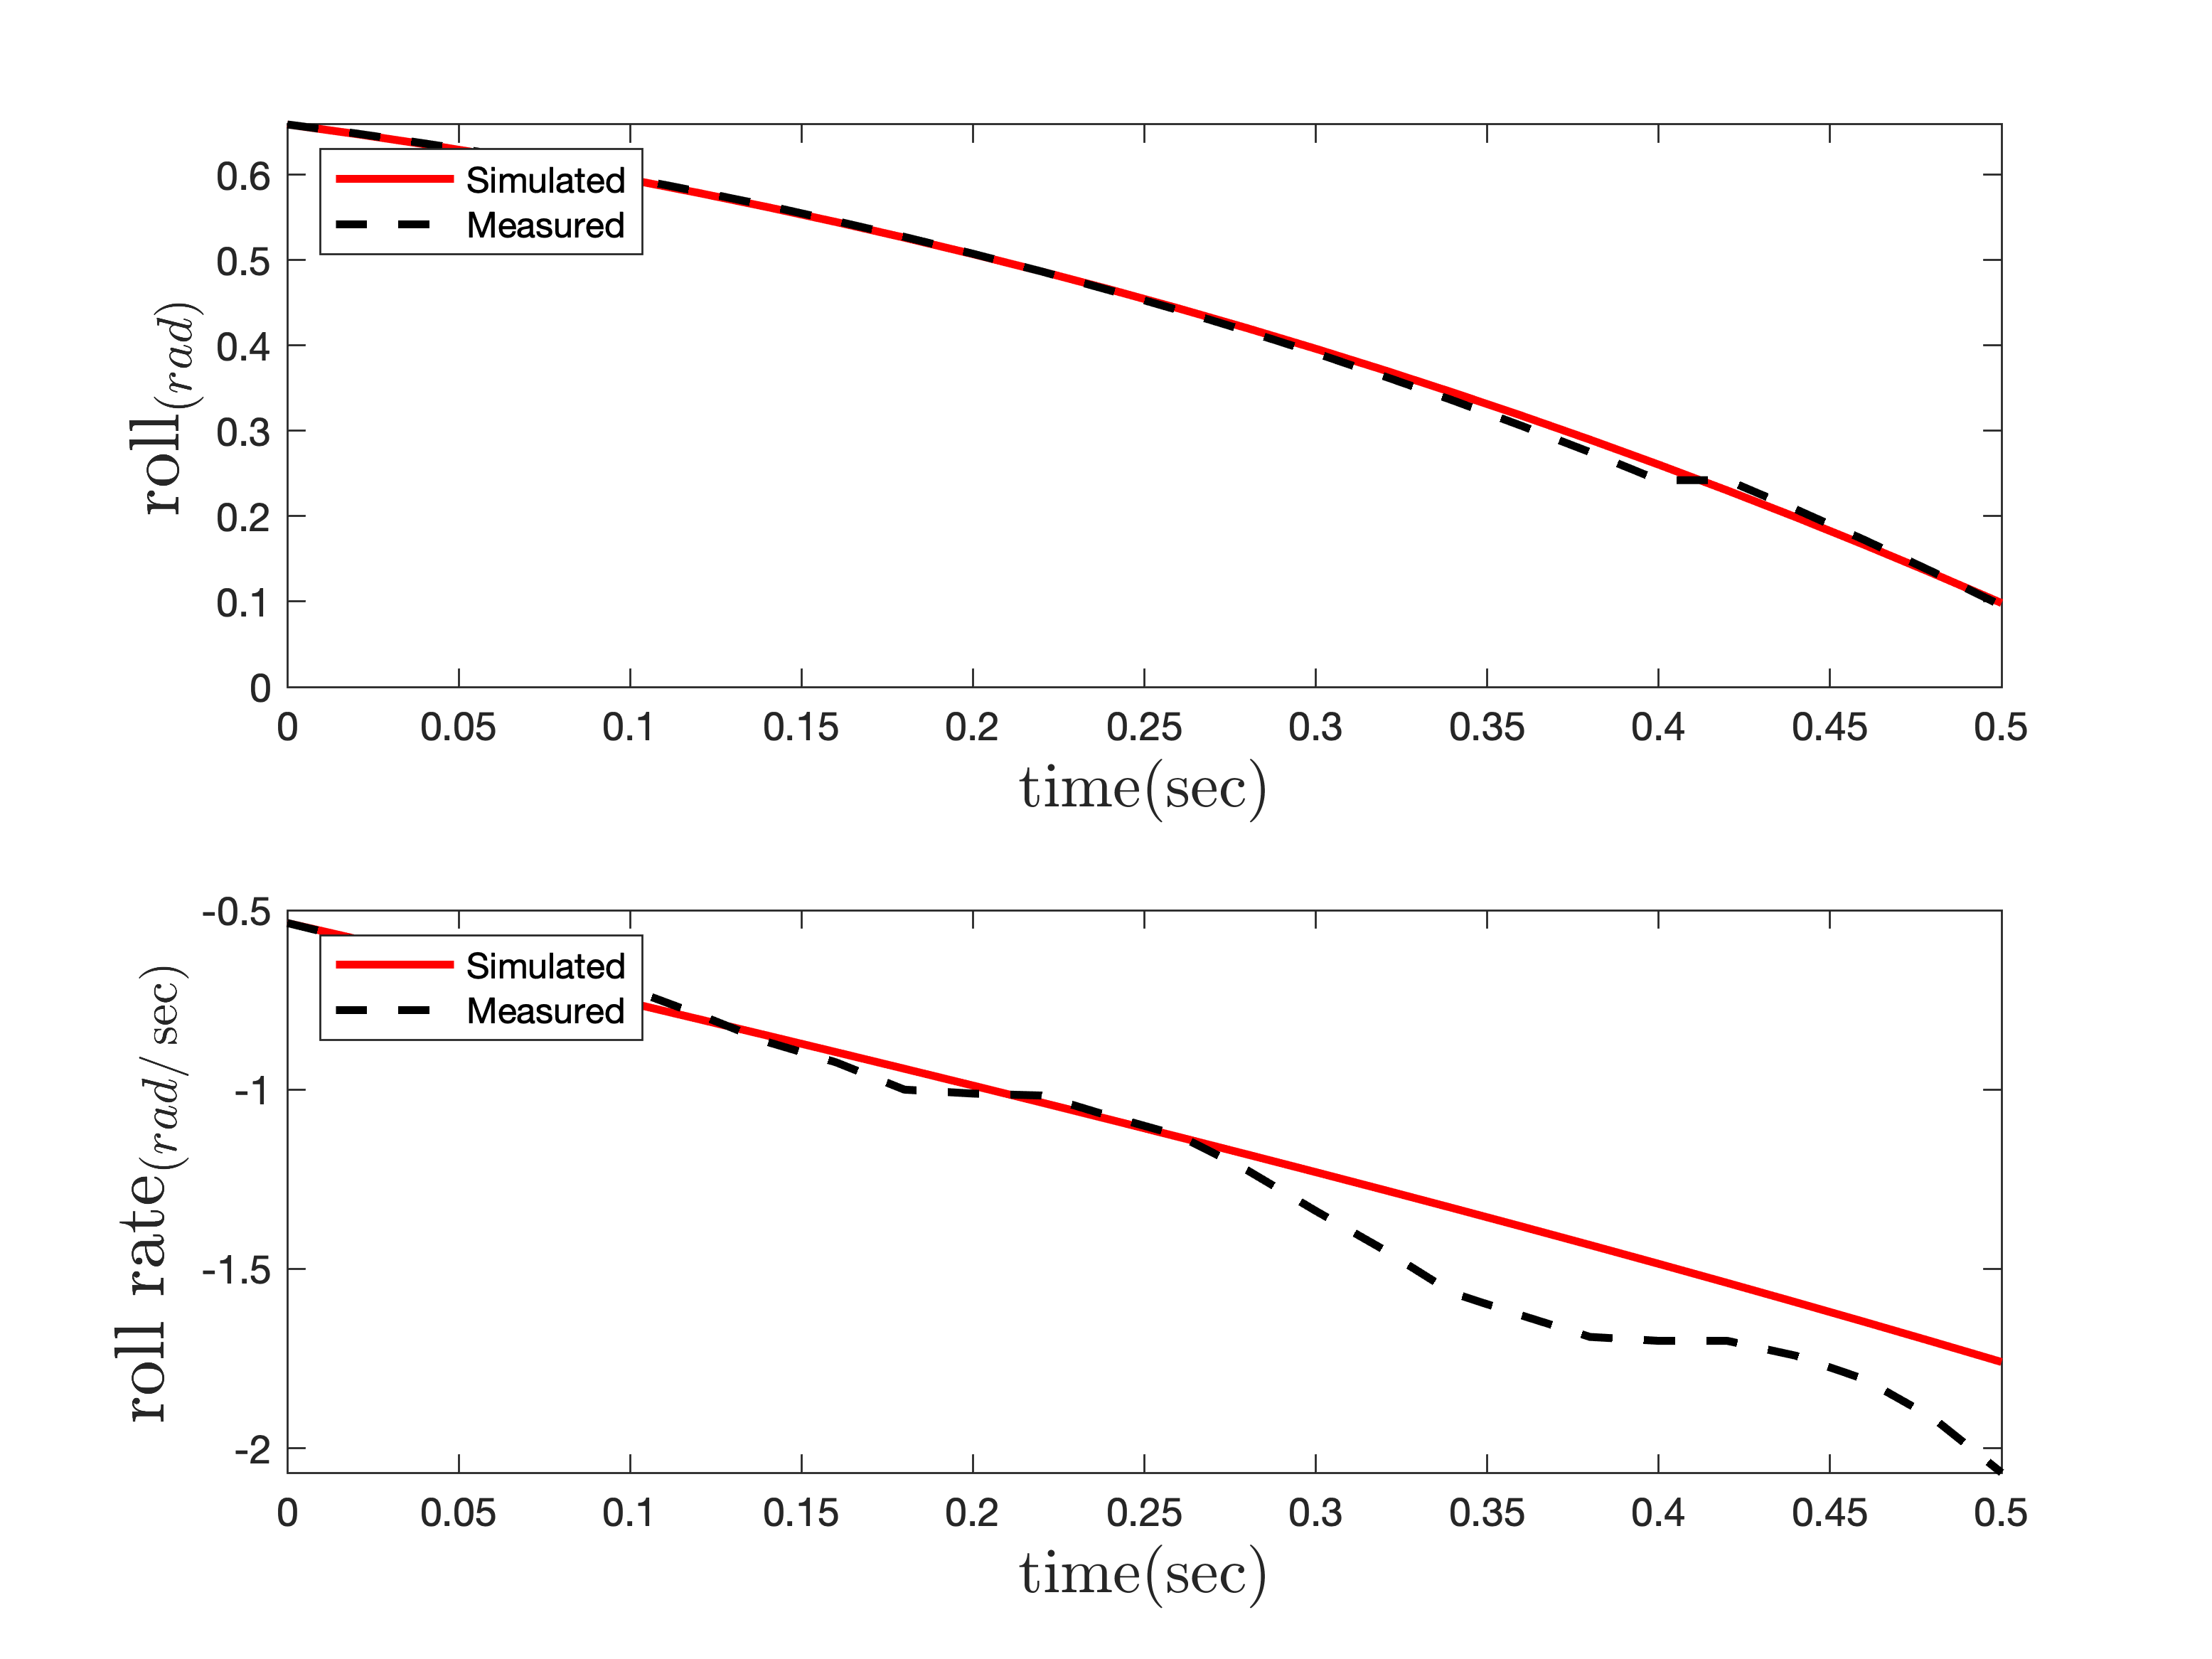
\includegraphics[width=2.3in]{../Figures/RCP/roll_parameter_estimation/RCP_roll_S4.png}
%     \label{fig: roll PE}}
%     \hfil
%     \subfloat[Pitch]{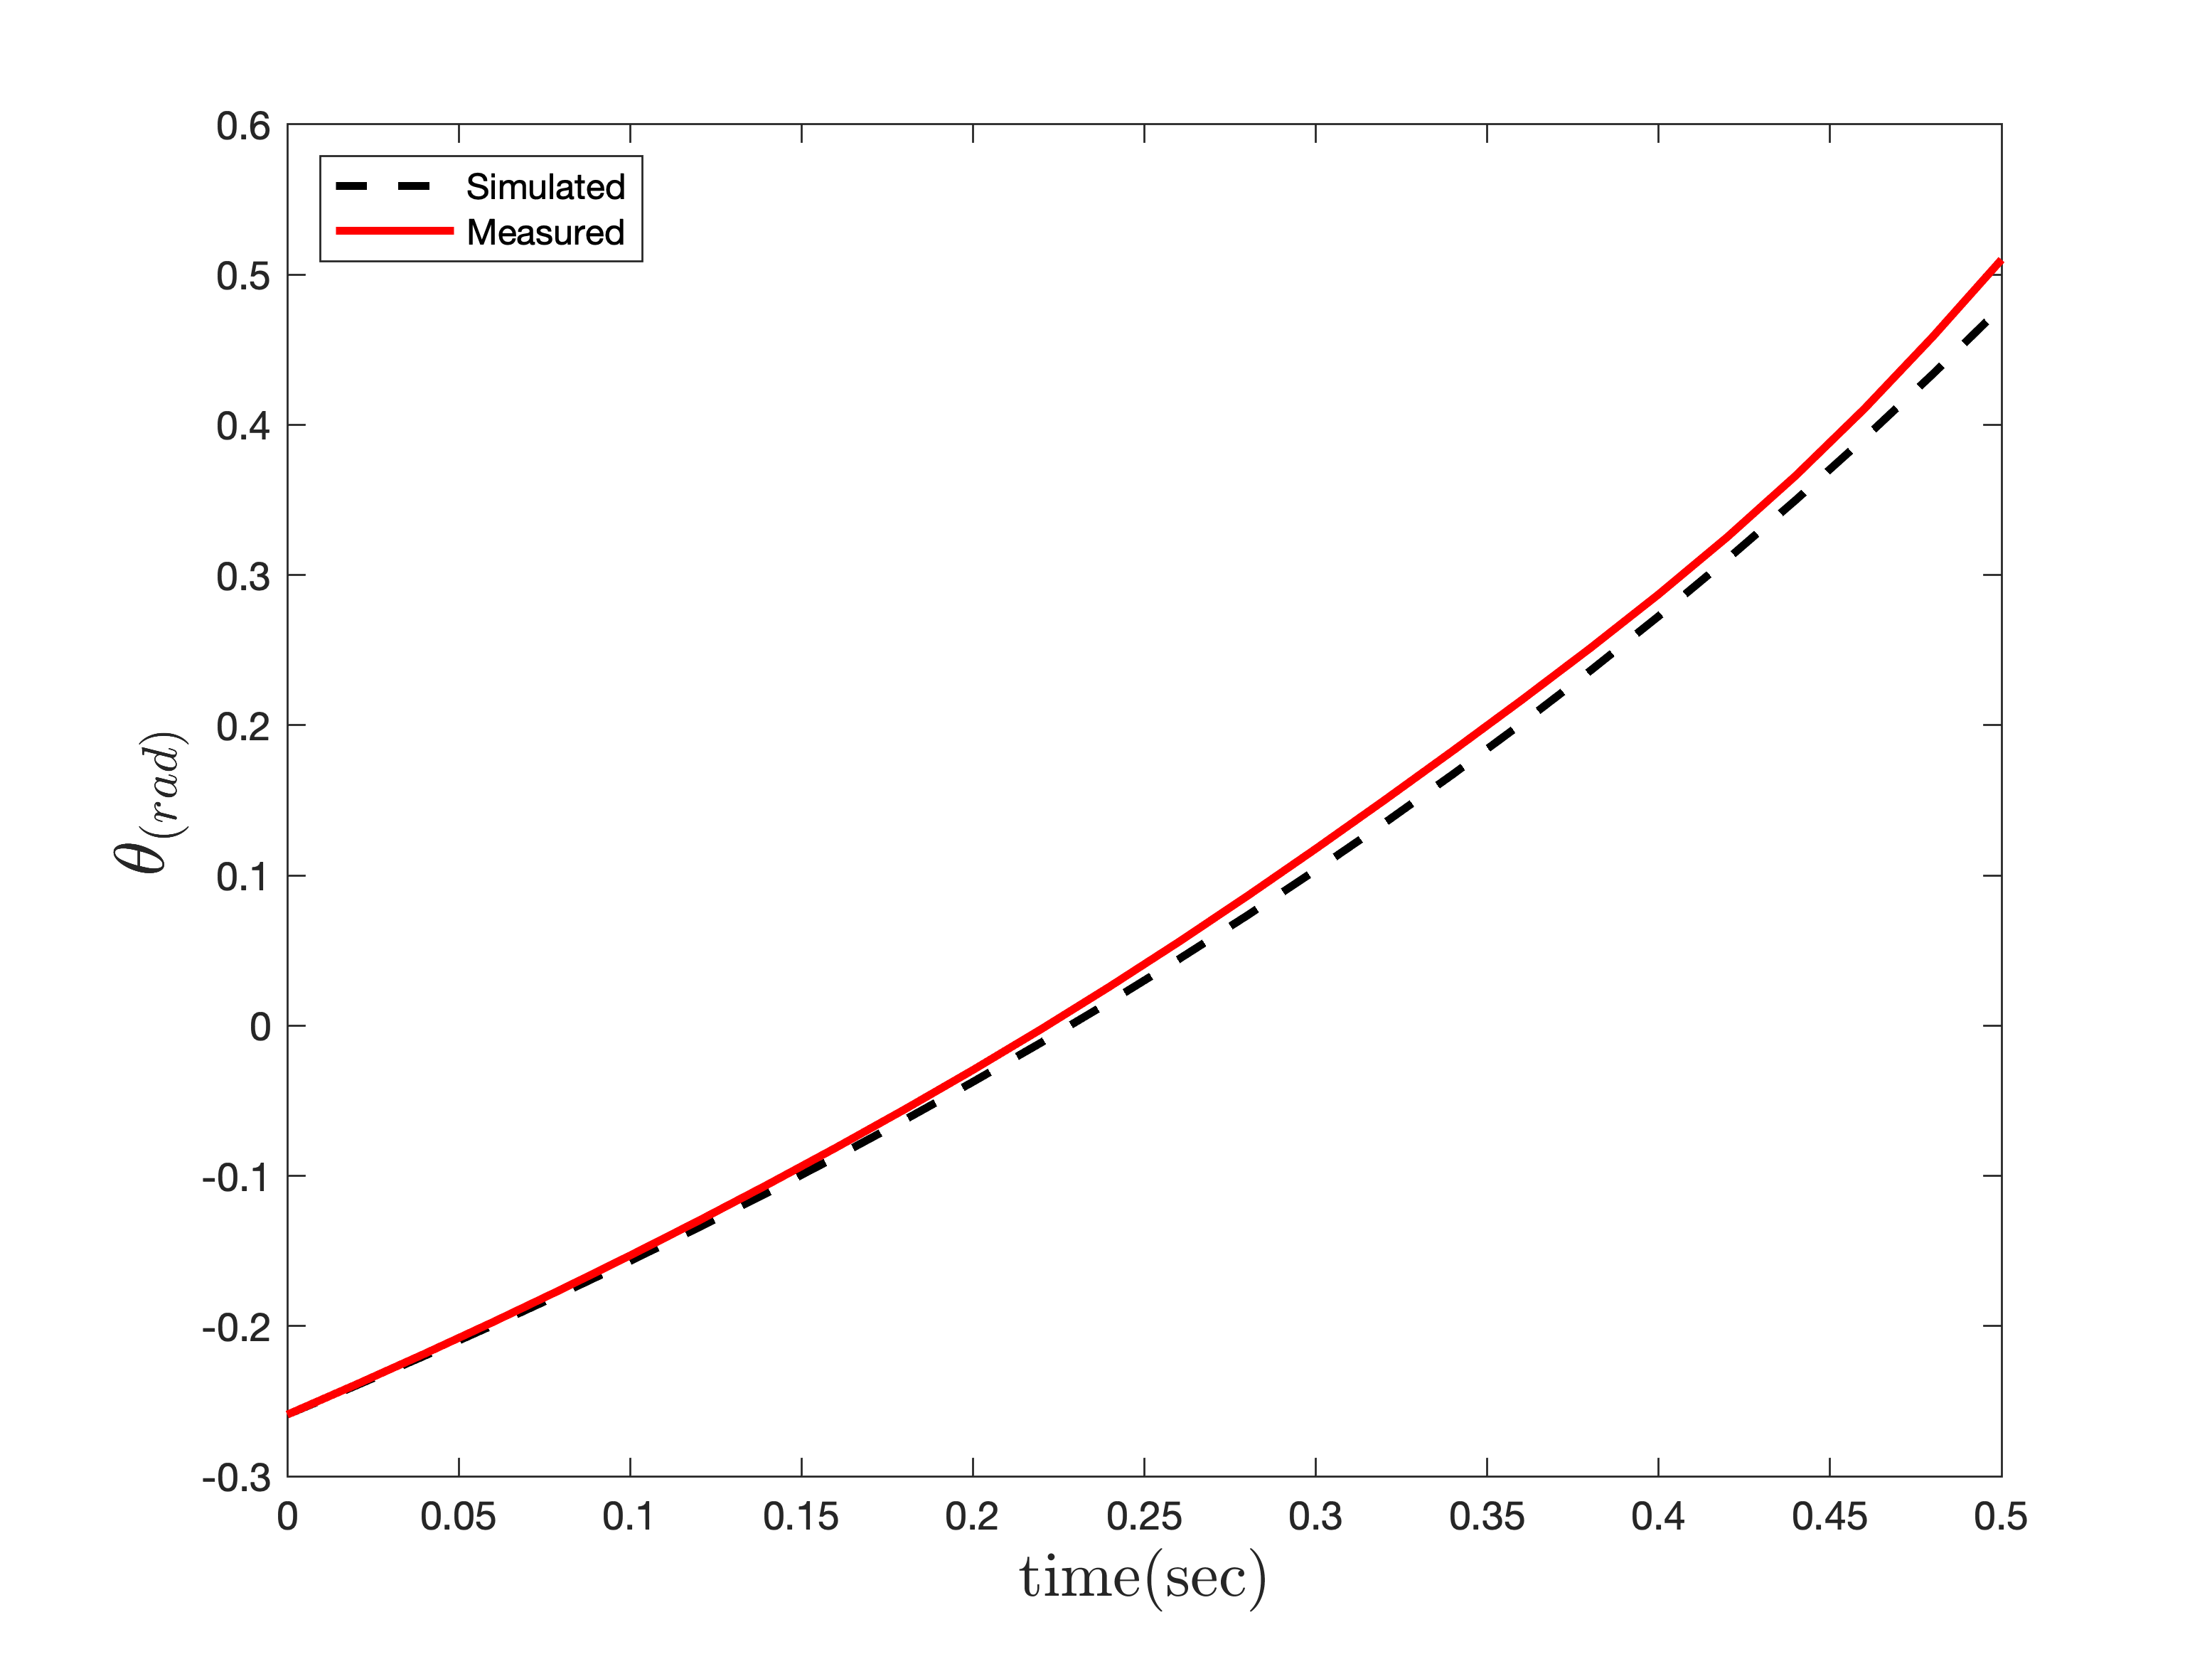
\includegraphics[width=2.3in]{../Figures/RCP/pitch_parameter_estimation/RCP_pitch_S1.png}
%     \label{fig: pitch PE}}
% 	\hfil
%     \subfloat[Yaw]{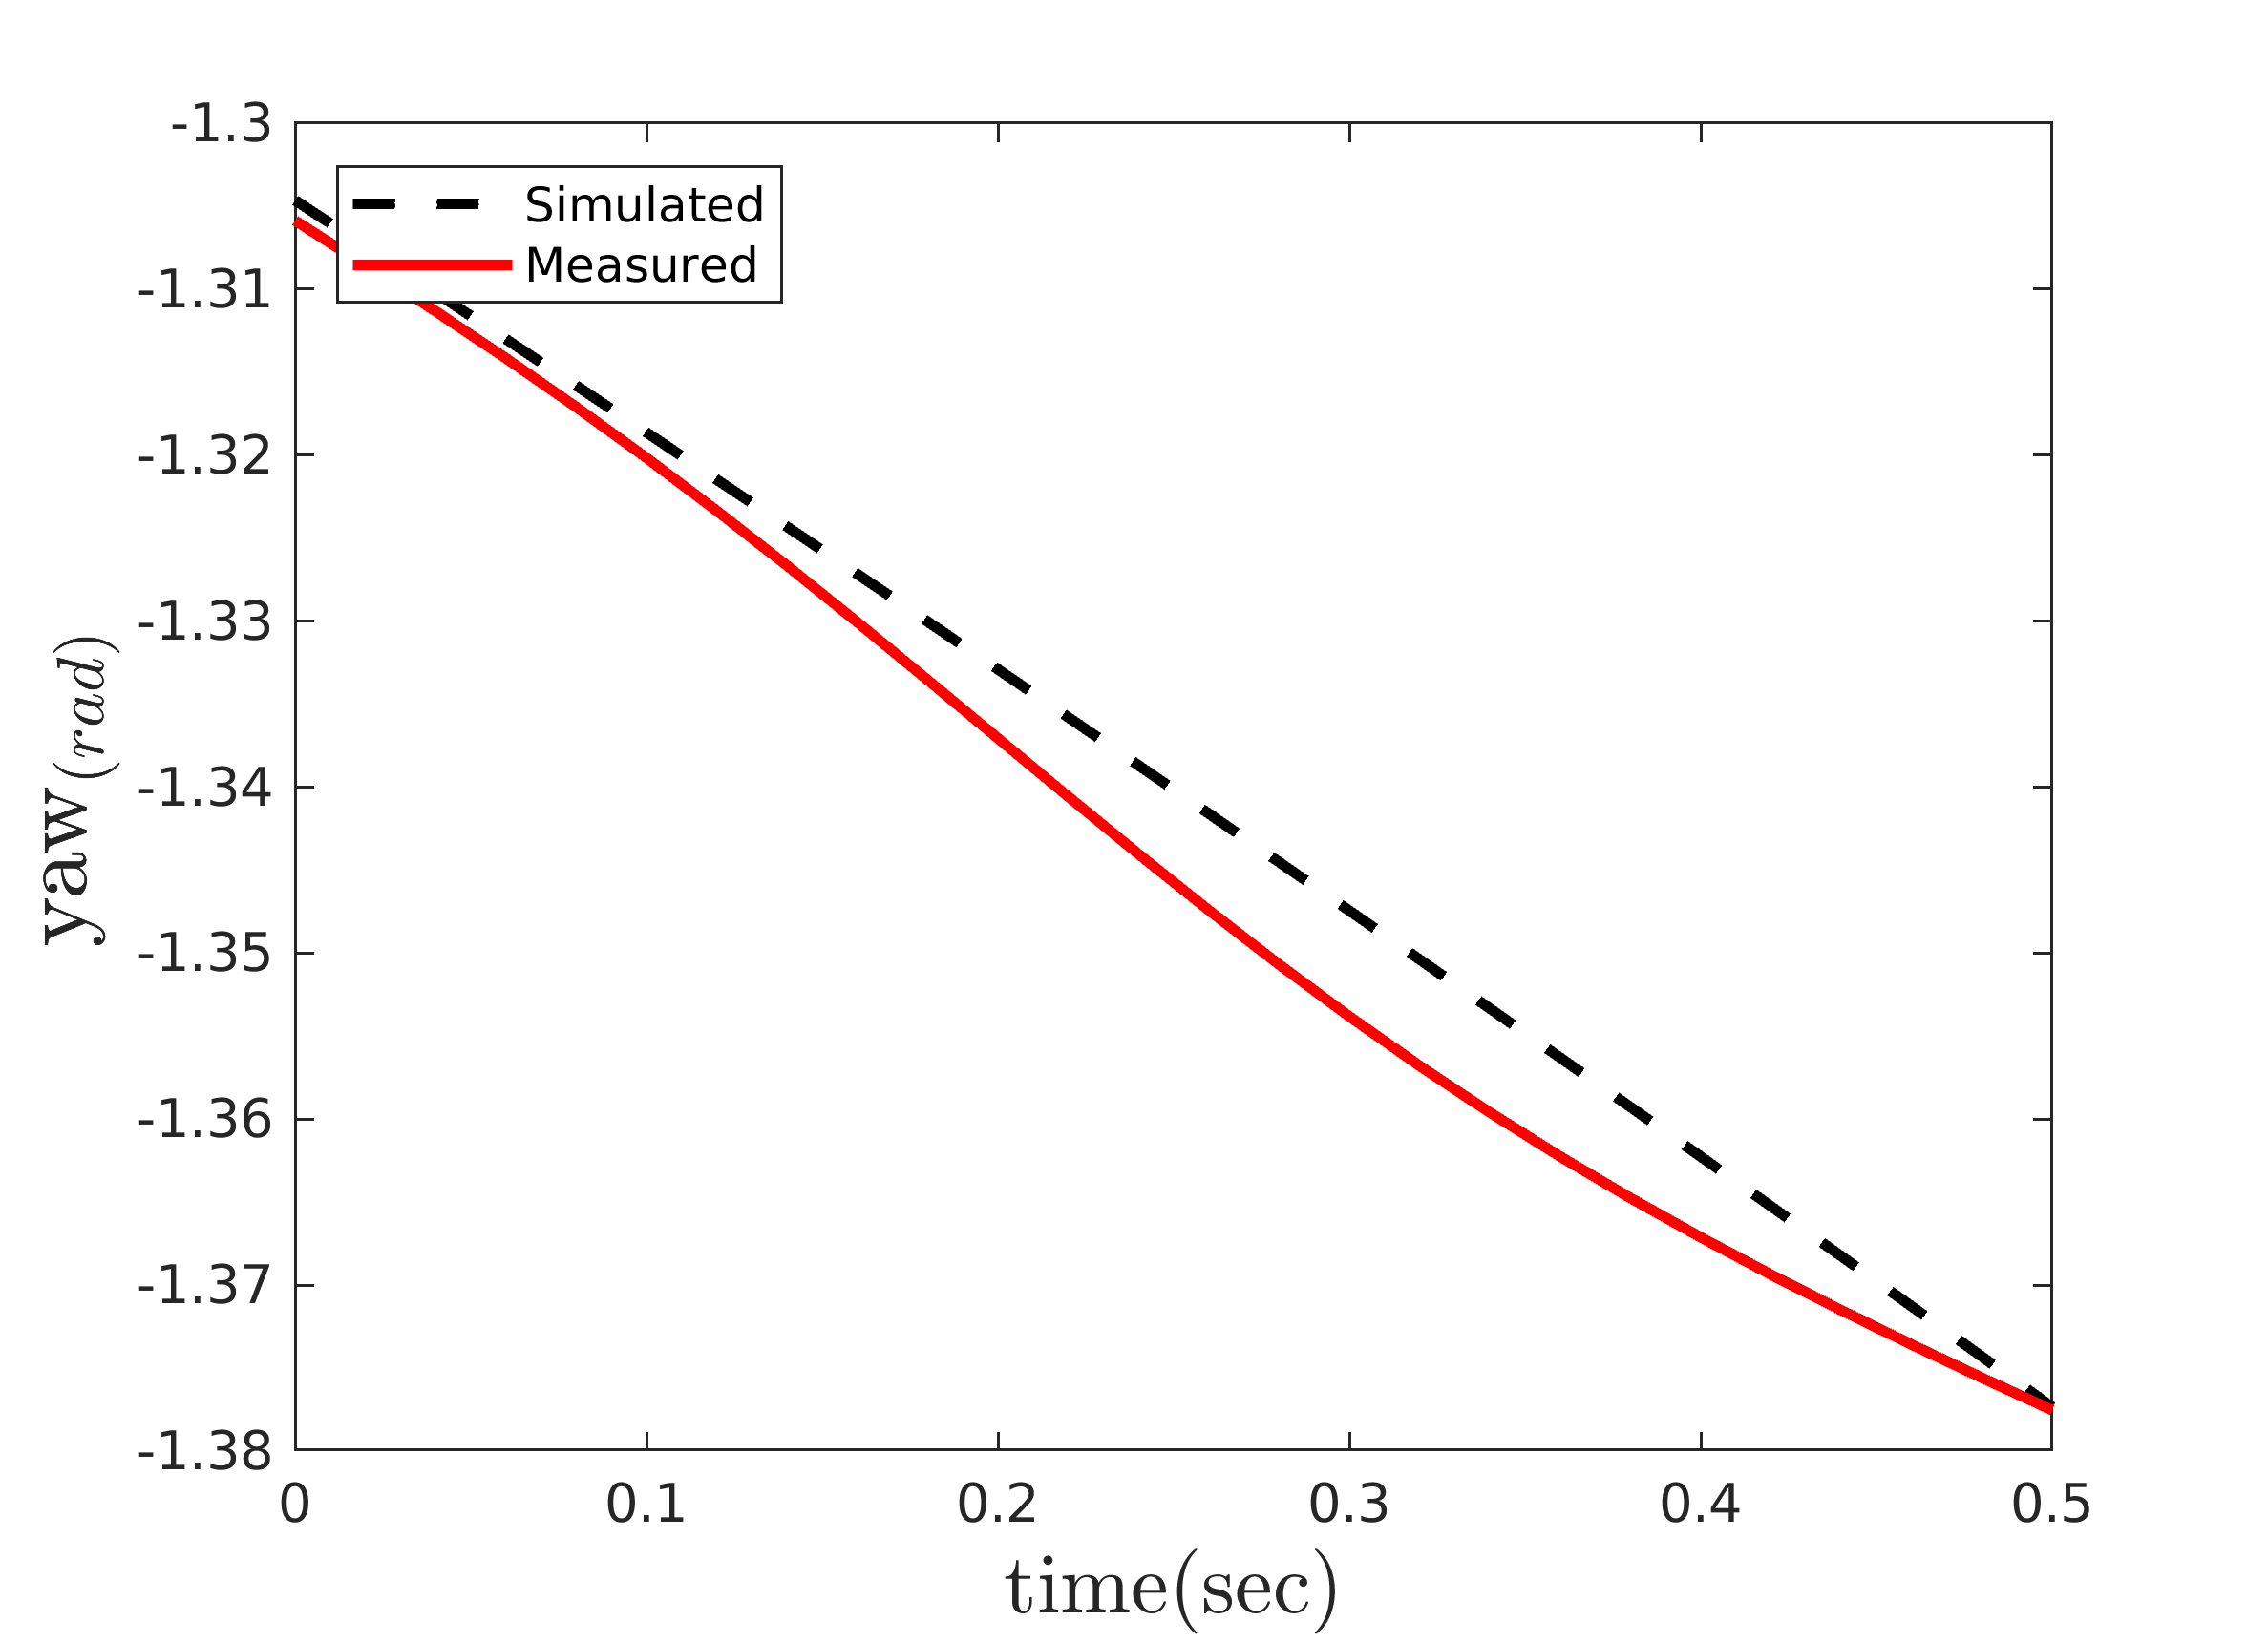
\includegraphics[width=2.3in]{../Figures/RCP/yaw_parameter_estimation/RCP_yaw_S2.png}
%     \label{fig: yaw PE}}
%     \caption{Simulation results for the network.} \label{fig_sim}
% \end{figure*}
% \subsection{Parameter Estimation}
% This section modifies the quadrotor stand parameters using the Simulink environment's simulation of different quadrotor channels and the stand's output data.
% % This section uses the output data from the quadrotor stand to modify the parameters of the quadrotor stand based on simulations of different quadrotor channels in Simulink.
% % In this section, the parameters of the quadrotor stand are modified by using the simulation of different quadrotor channels in the Simulink environment and the output data from the quadrotor stand.
% The quadrotor stand parameters have been modified using the Parameter Estimator toolbox available in the Simulink environment.
% % The Parameter Estimator toolbox has been used in the Simulink environment to modify the quadrotor stand parameters.
% % The Parameter Estimator toolbox available in the Simulink environment has been used to modify the parameters of the quadrotor stand.
% In order to perform the test, the quadrotor stand was released from various initial conditions and inputs, and data was collected using the output from the sensor.
% % In order to conduct the test, the quadrotor stand was released from different initial conditions and inputs, and the sensor's output was used to collect data.
% % The quadrotor stand was released from different initial conditions and inputs to perform the test, and data was collected from the sensor's output.
% Then, Parameter Estimator takes the model and the recorded data of the sensor (stand states).
% %  Then, the model and the recorded data of the sensor (state of the stand) are given to the Parameter Estimator toolbox.
% Here is a comparison between the states of the quadrotor in simulation and reality after modifying various parameters.
% % Below is a comparison of how the quadrotor performed in simulations and real-life after modifying various parameters.
% % The state of the quadrotor stand in simulation and reality after modifying various parameters is compared below.

% \begin{figure*}[!h]
% 	\centering
% 	\subfloat[Roll Channel]{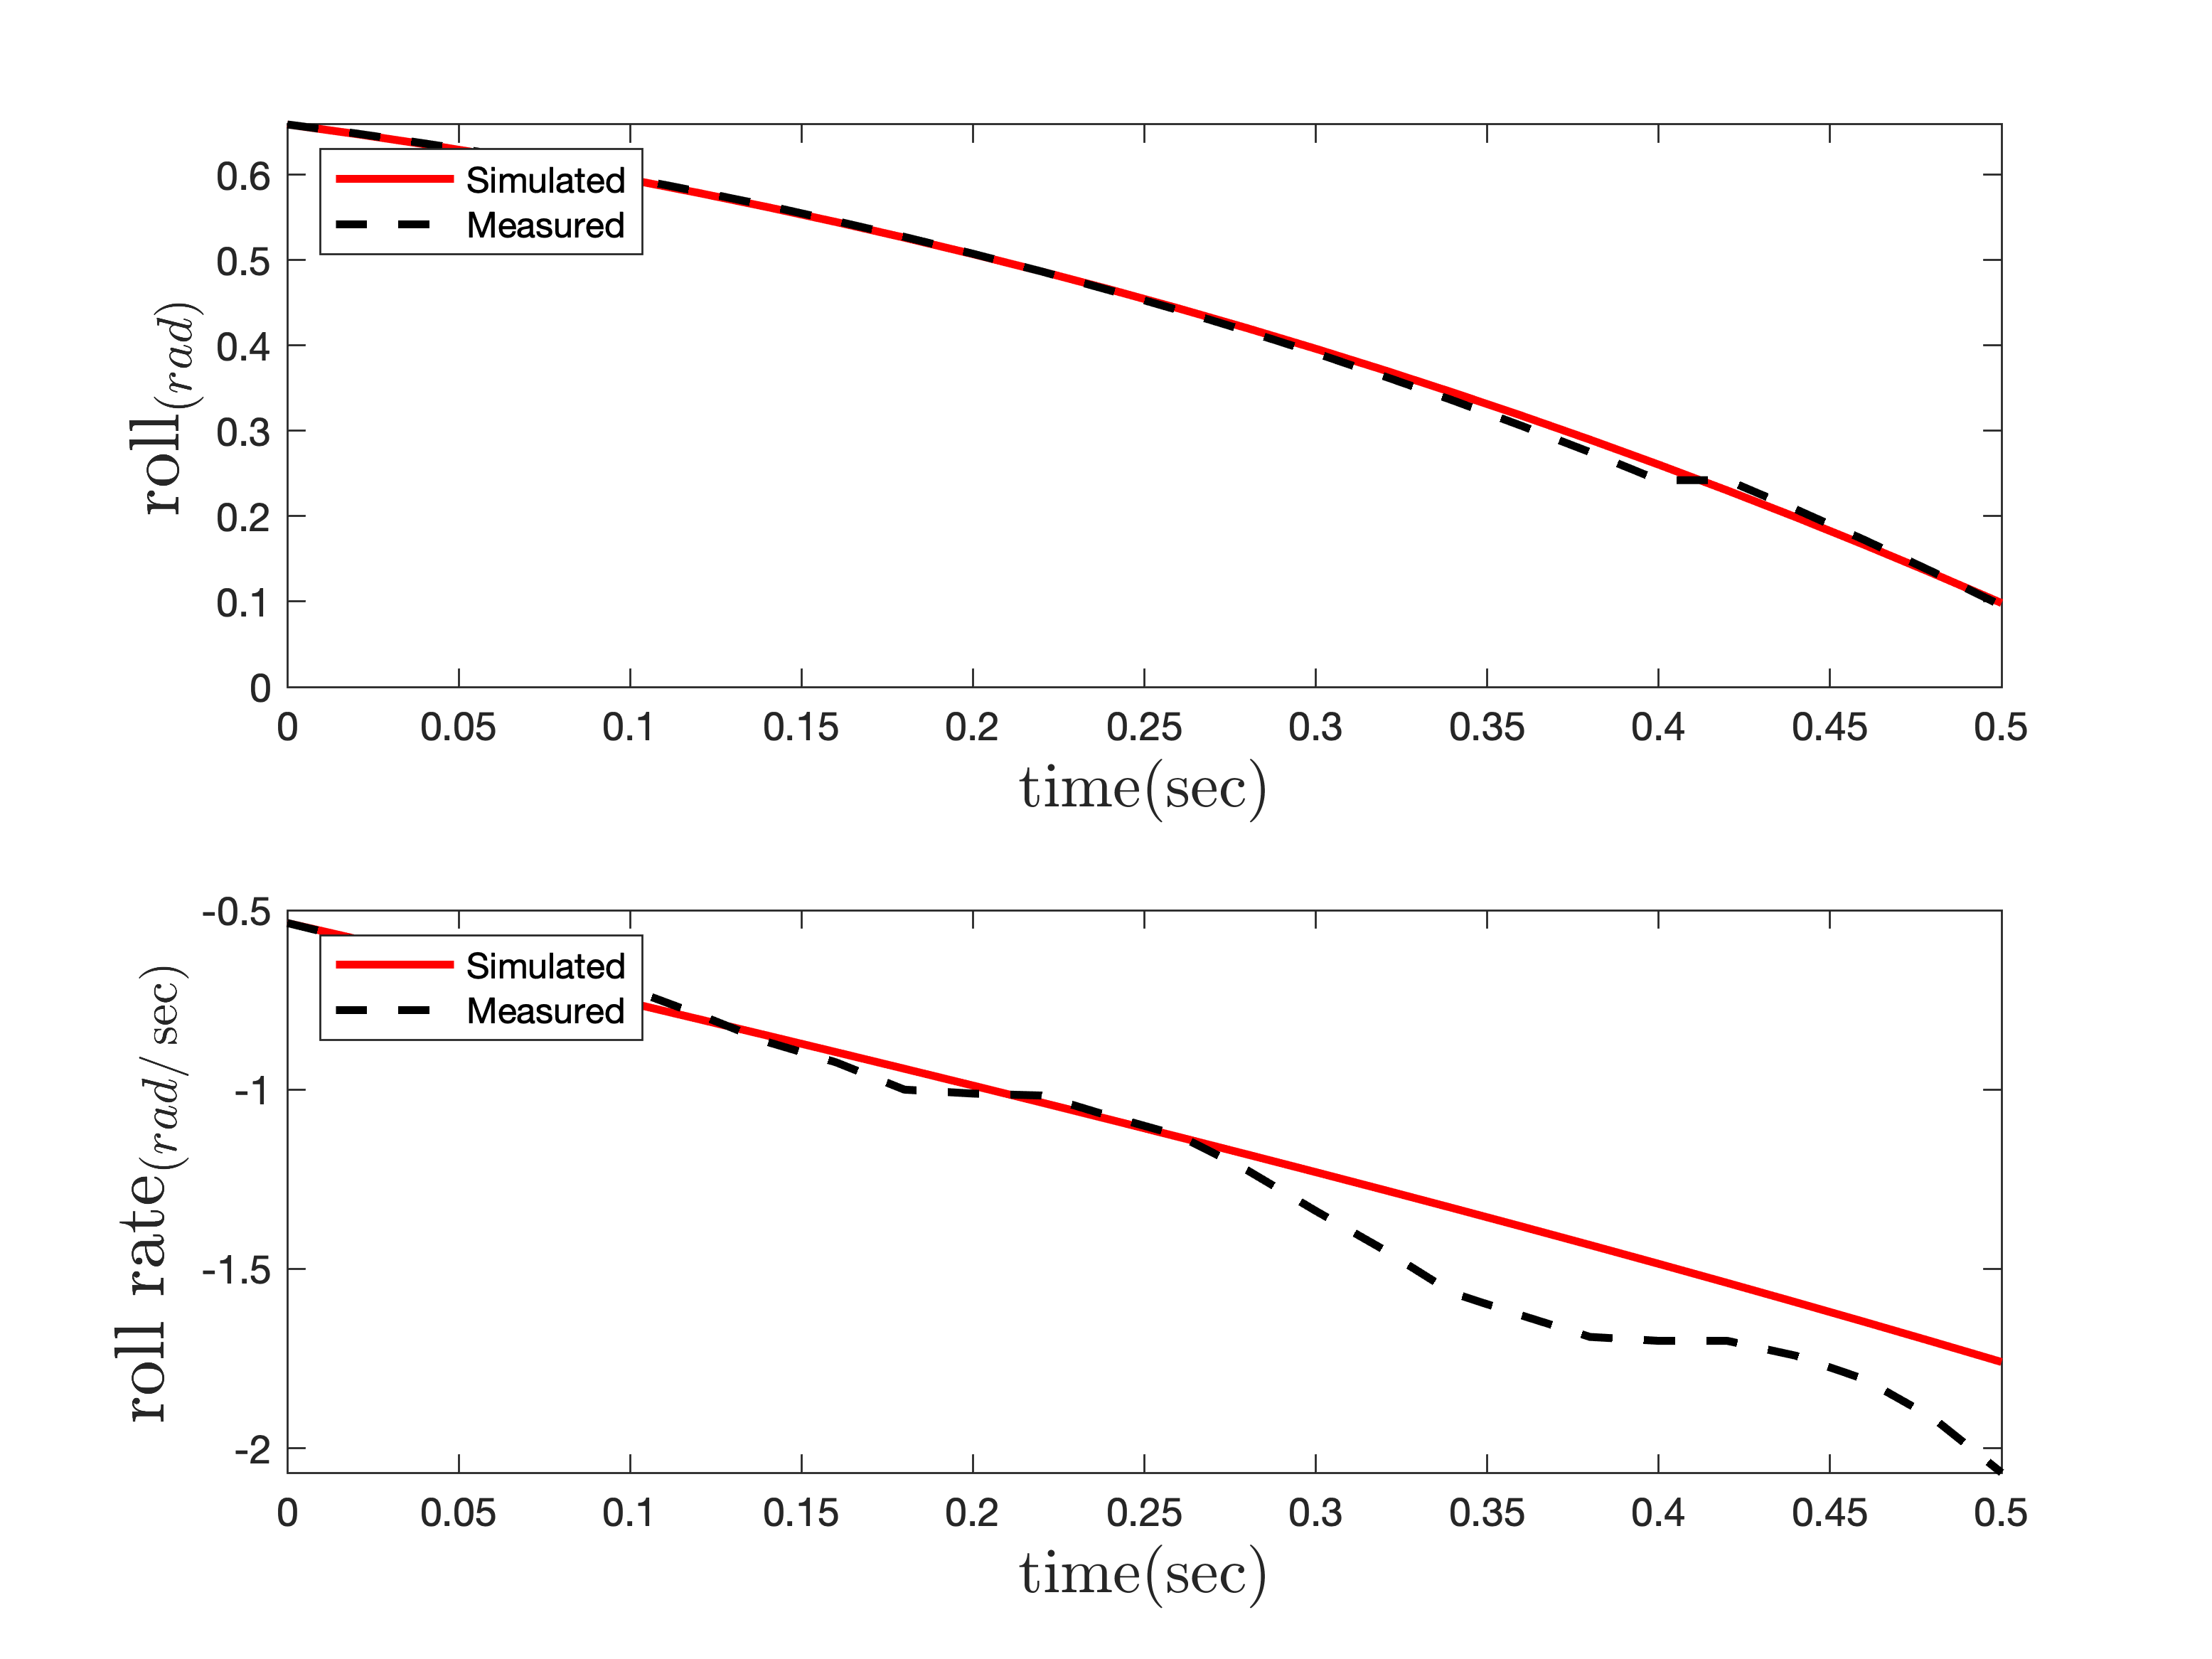
\includegraphics[width=2.3in]{../Figures/RCP/roll_parameter_estimation/RCP_roll_S4.png}
% 	\label{fig: roll PE}}
% 	\hfil
% 	\subfloat[Pitch Channel]{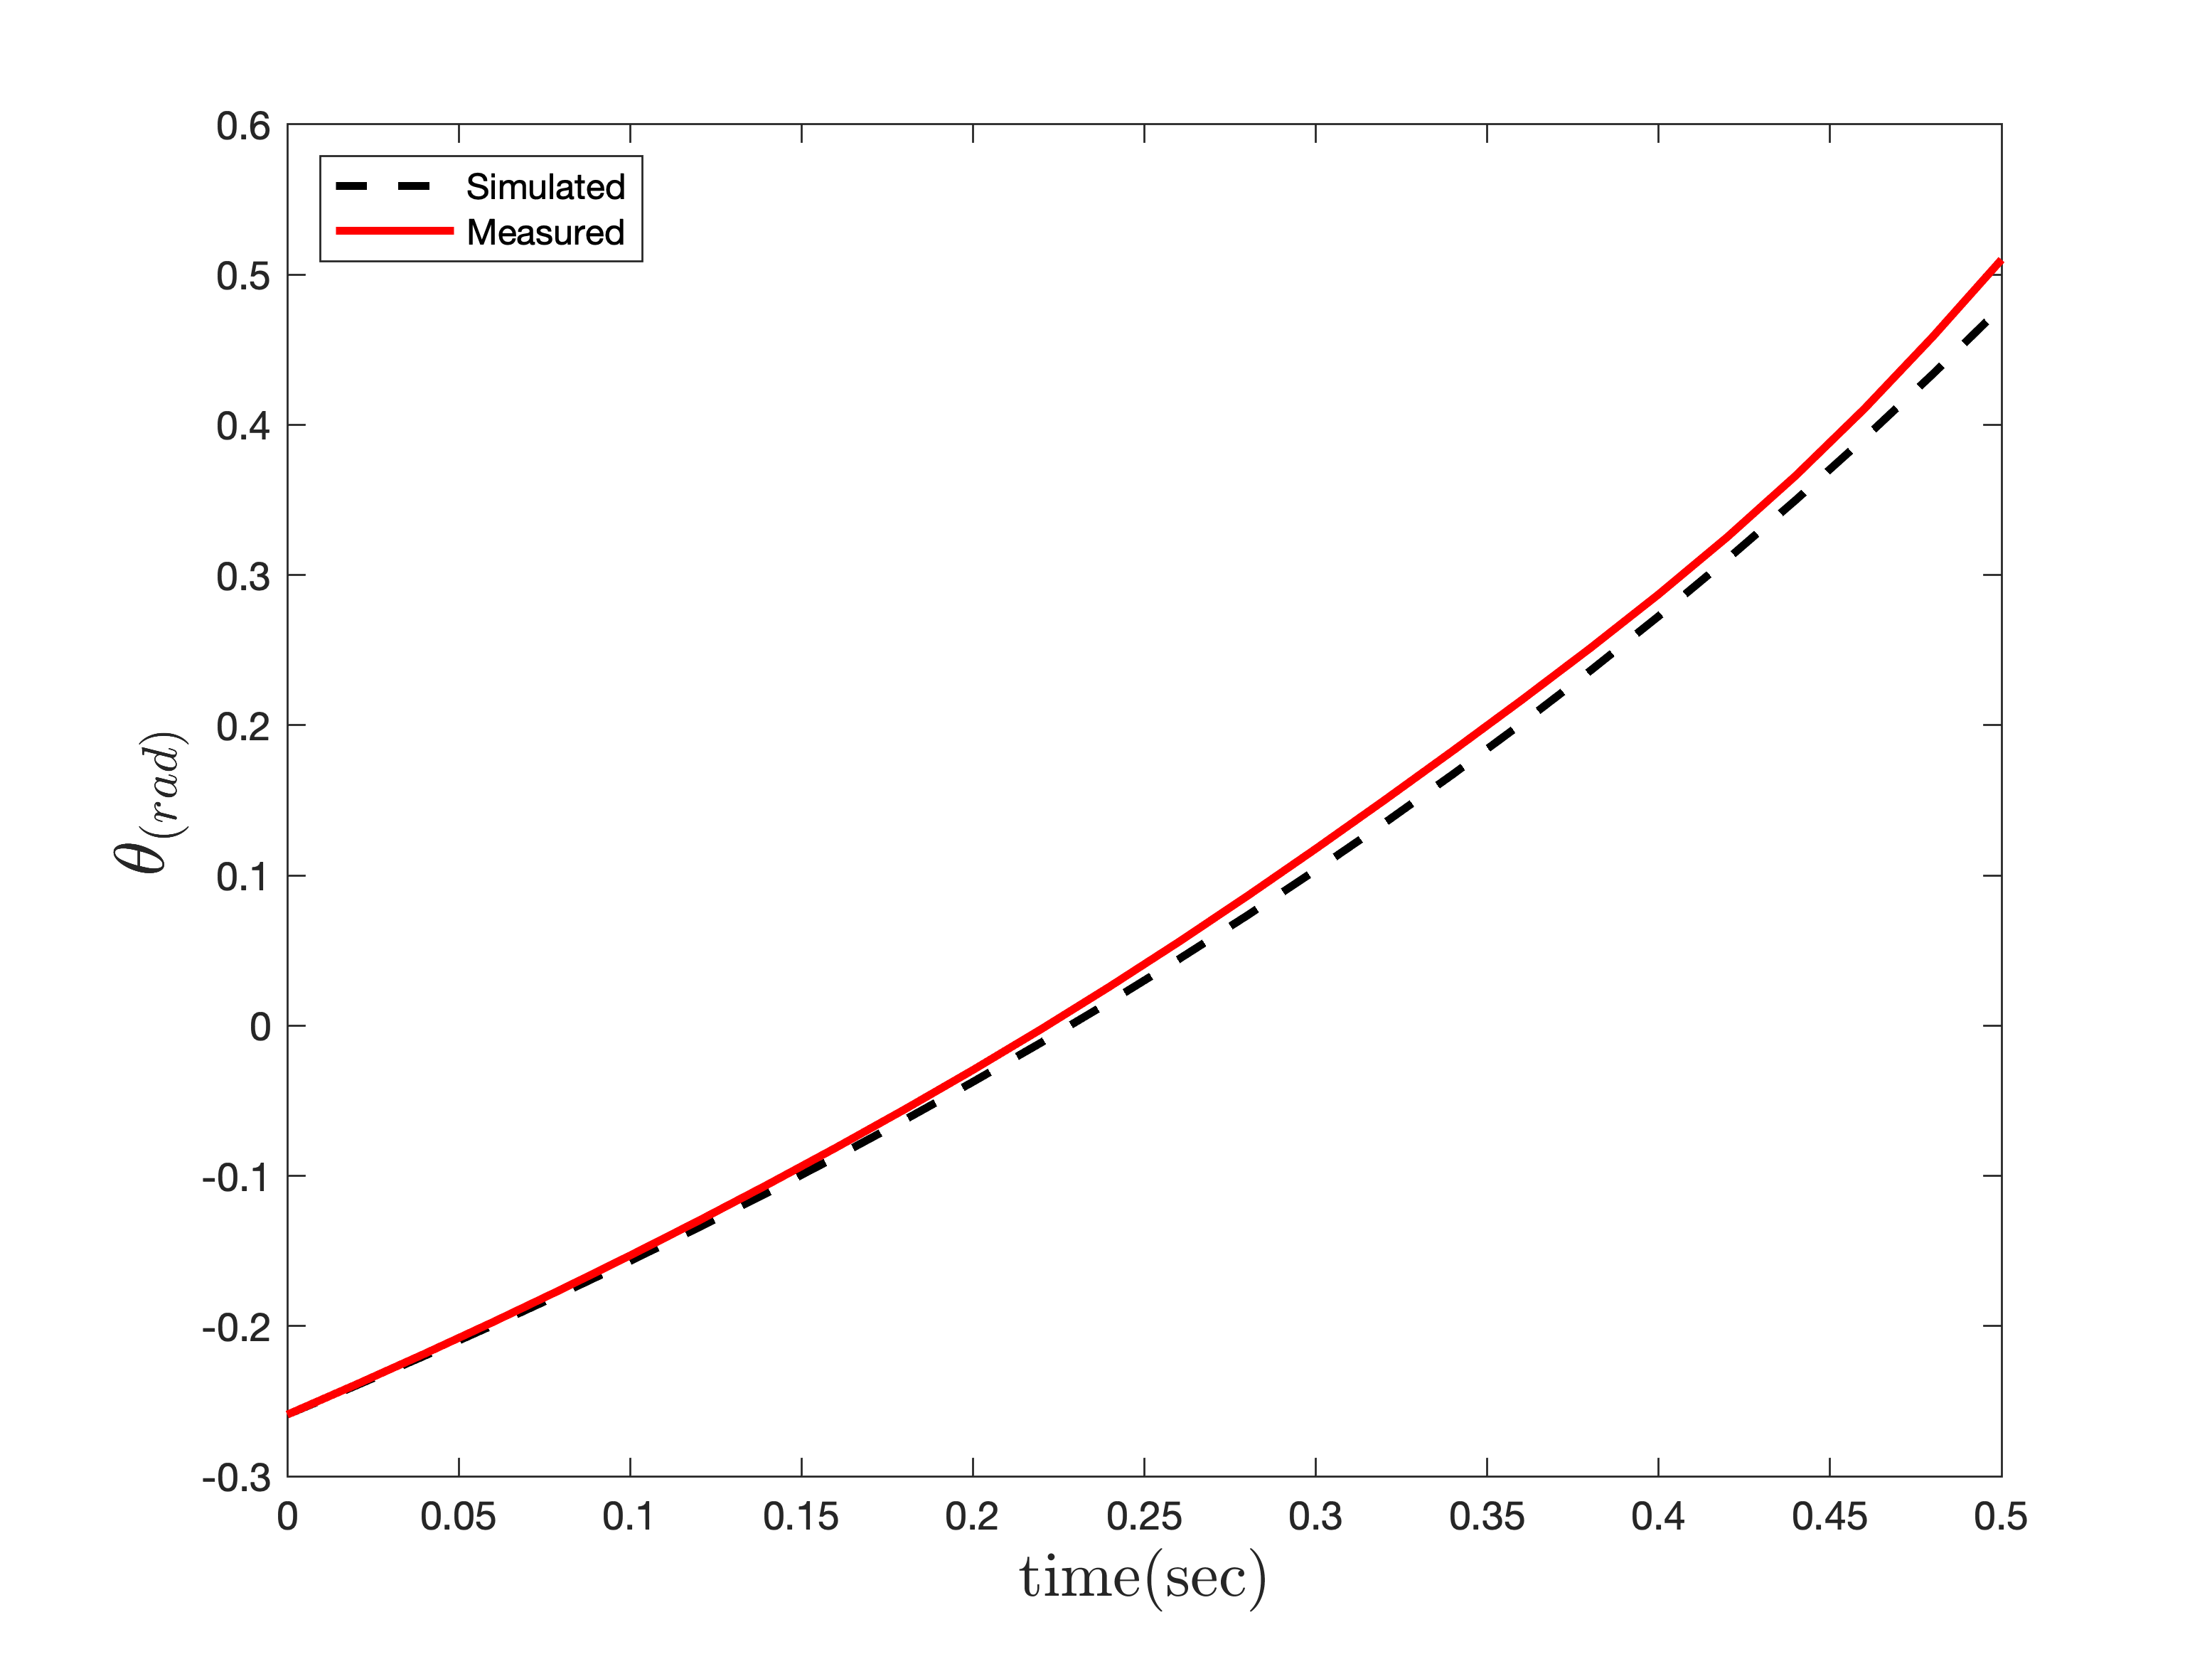
\includegraphics[width=2.3in]{../Figures/RCP/pitch_parameter_estimation/RCP_pitch_S1.png}
% 	\label{fig: pitch PE}}
% 	\hfil
% 	\subfloat[Yaw Channel]{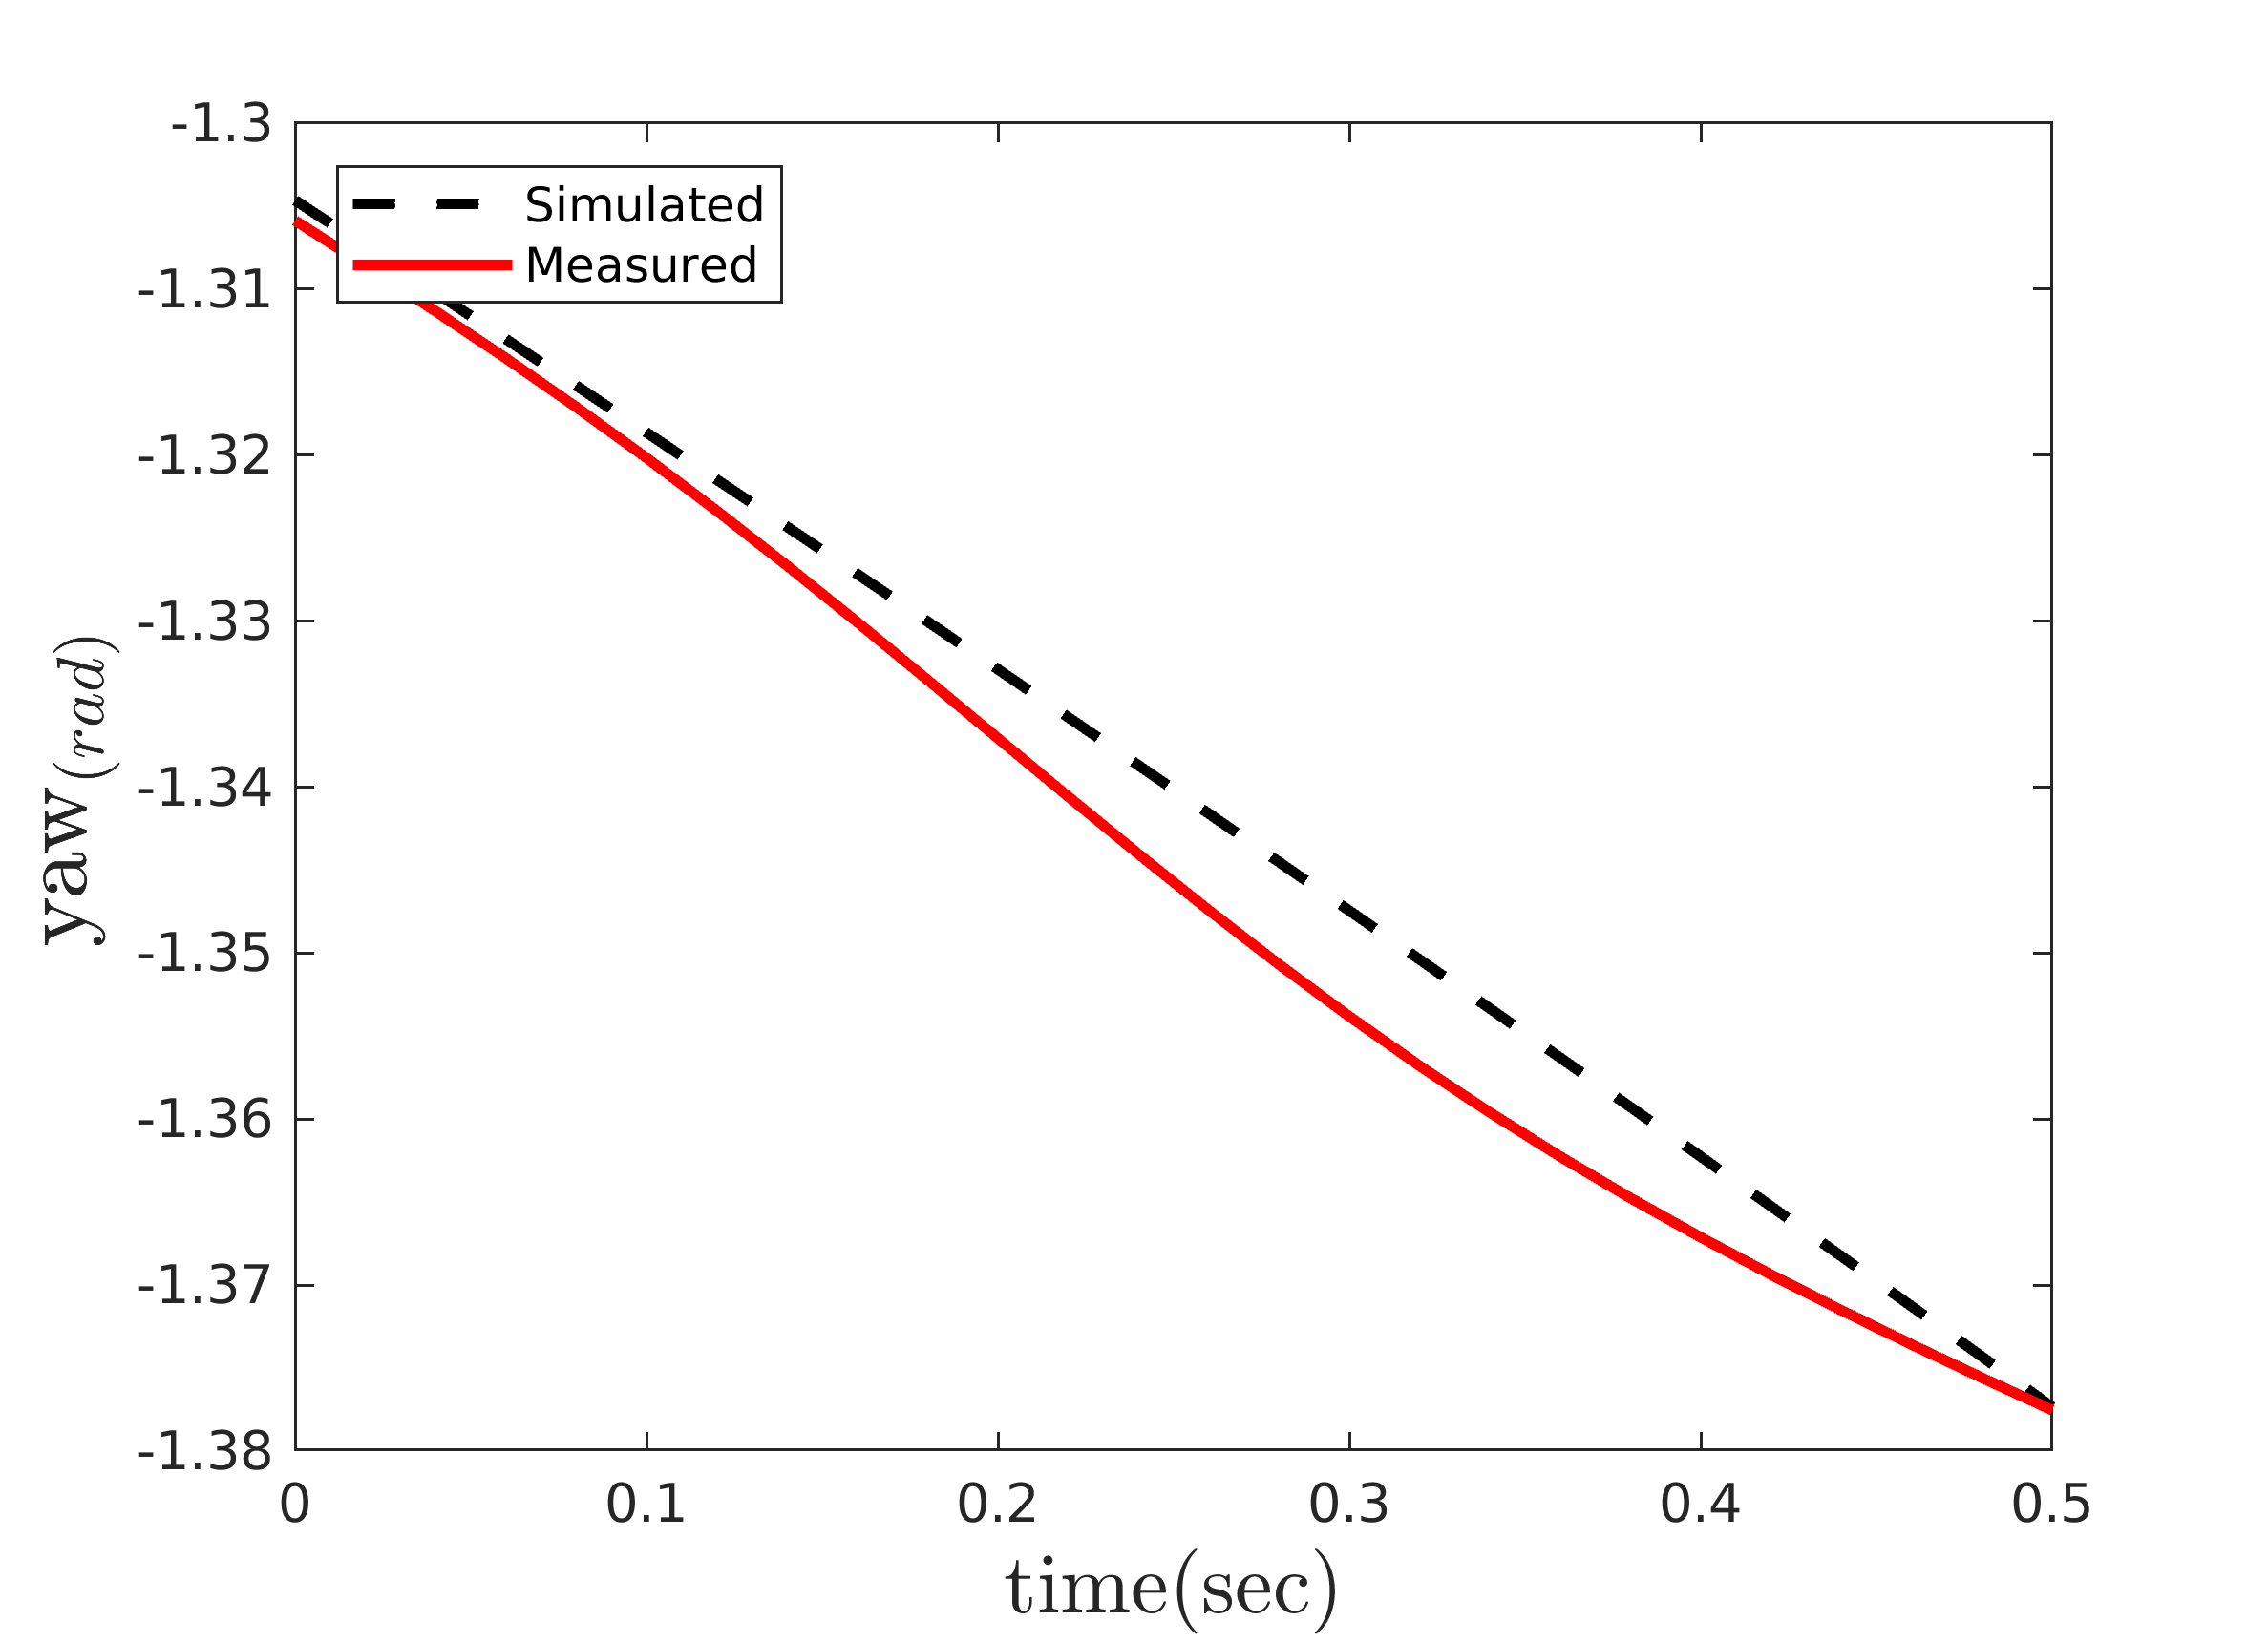
\includegraphics[width=2.3in]{../Figures/RCP/yaw_parameter_estimation/RCP_yaw_S2.png}
% 	\label{fig: yaw PE}}
% 	\caption{Comparison of quadrotor states in simulation and reality.} \label{fig_sim}
% \end{figure*}





% \begin{figure*}[htbp]
% 	\centering
% 	\subfloat[Roll]{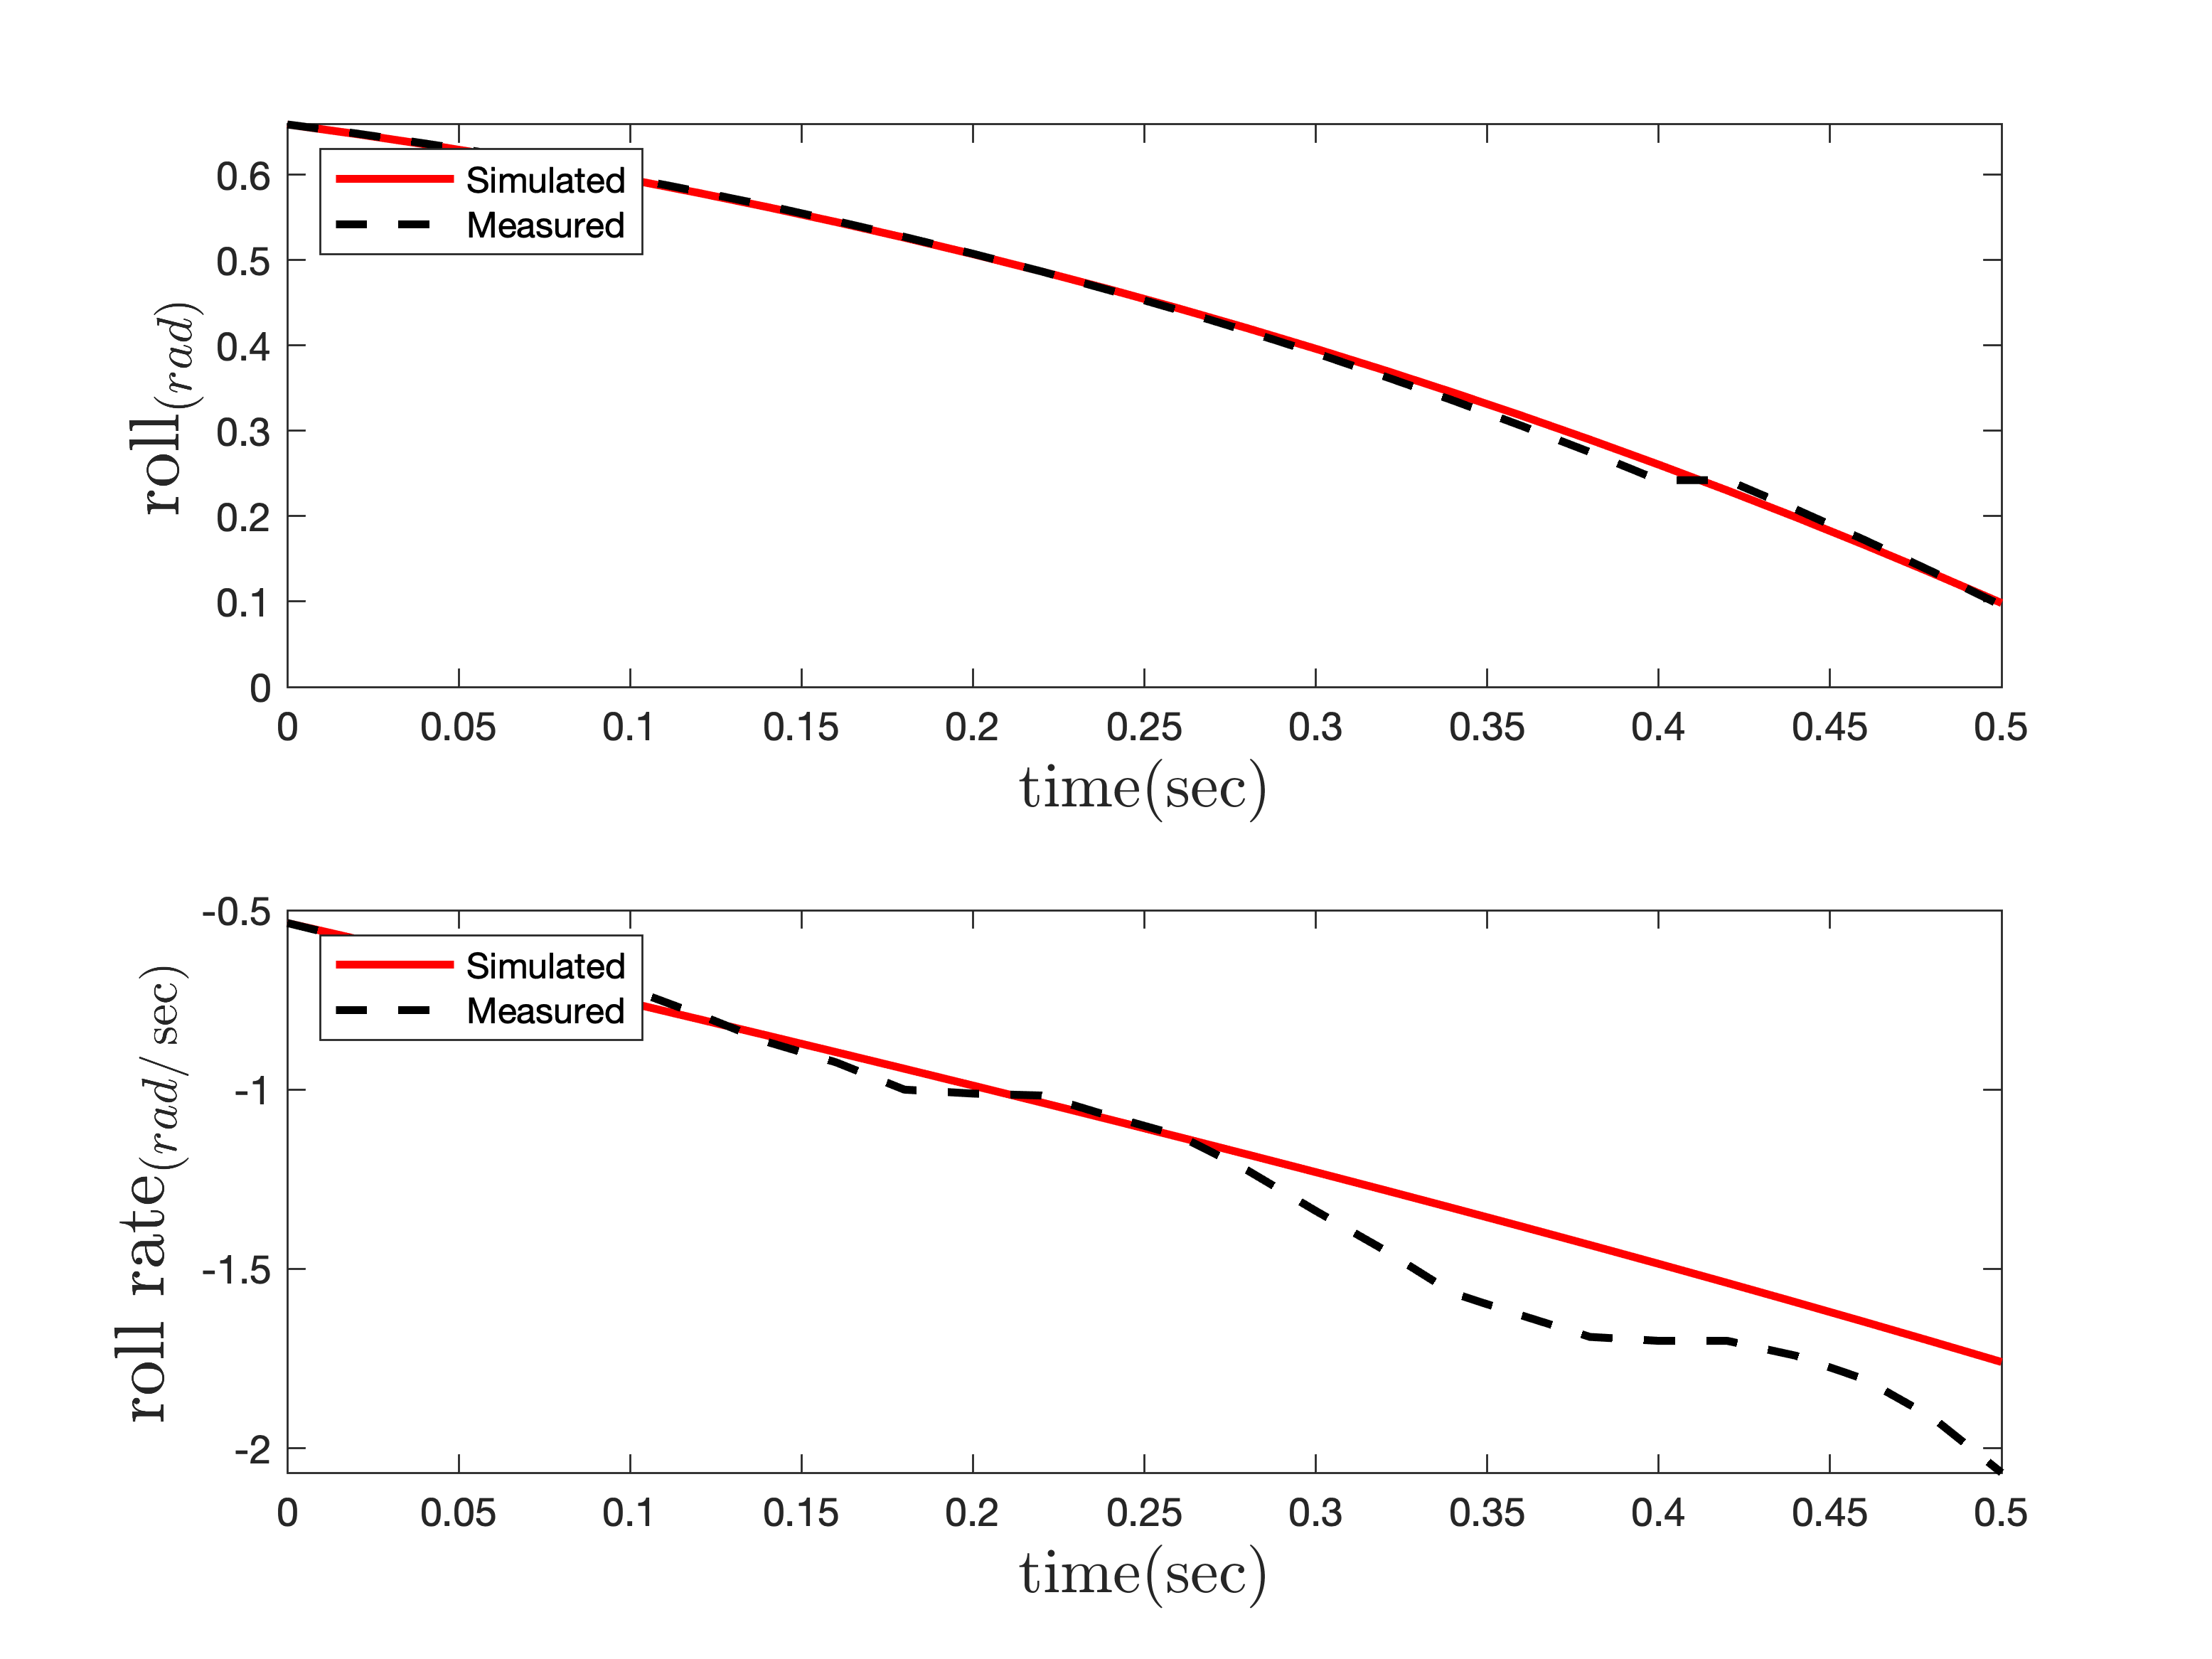
\includegraphics[width=2.3in]{../Figures/RCP/roll_parameter_estimation/RCP_roll_S4.png}
% 	\label{fig: roll PE}}
% 	\hfil
% 	\subfloat[Pitch]{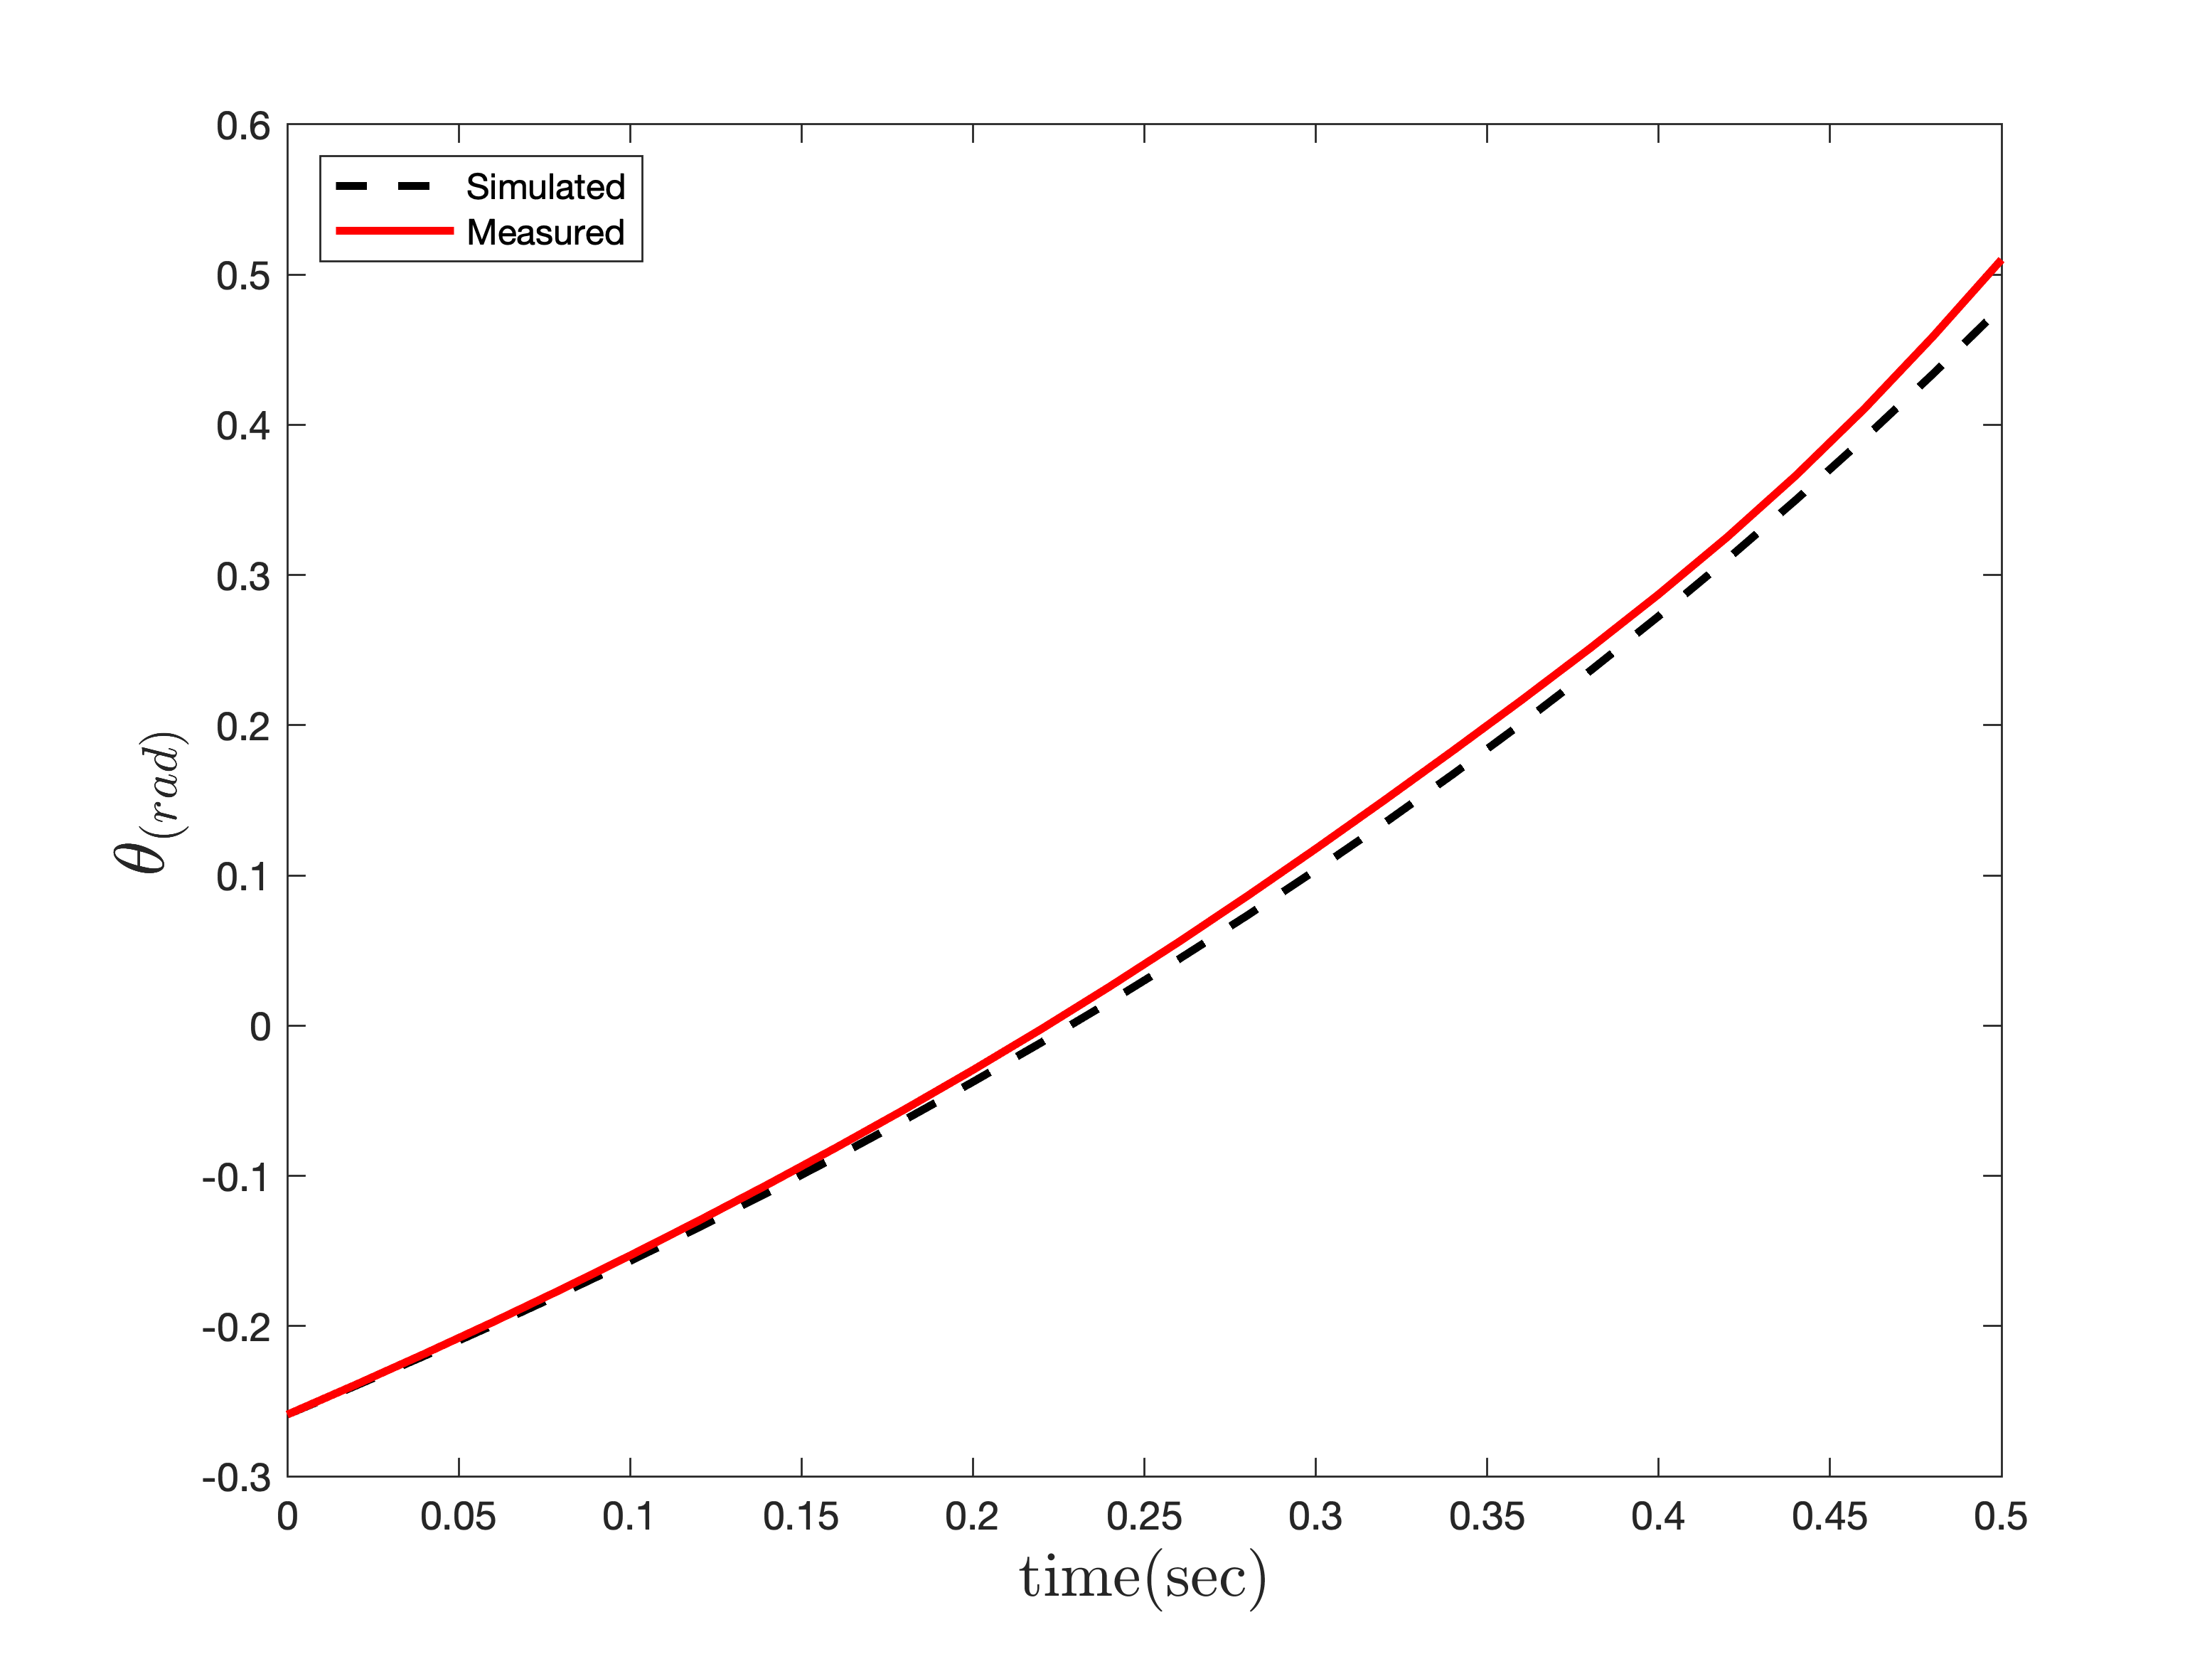
\includegraphics[width=2.3in]{../Figures/RCP/pitch_parameter_estimation/RCP_pitch_S1.png}
% 	\label{fig: pitch PE}}
% 	\hfil
% 	\subfloat[Yaw]{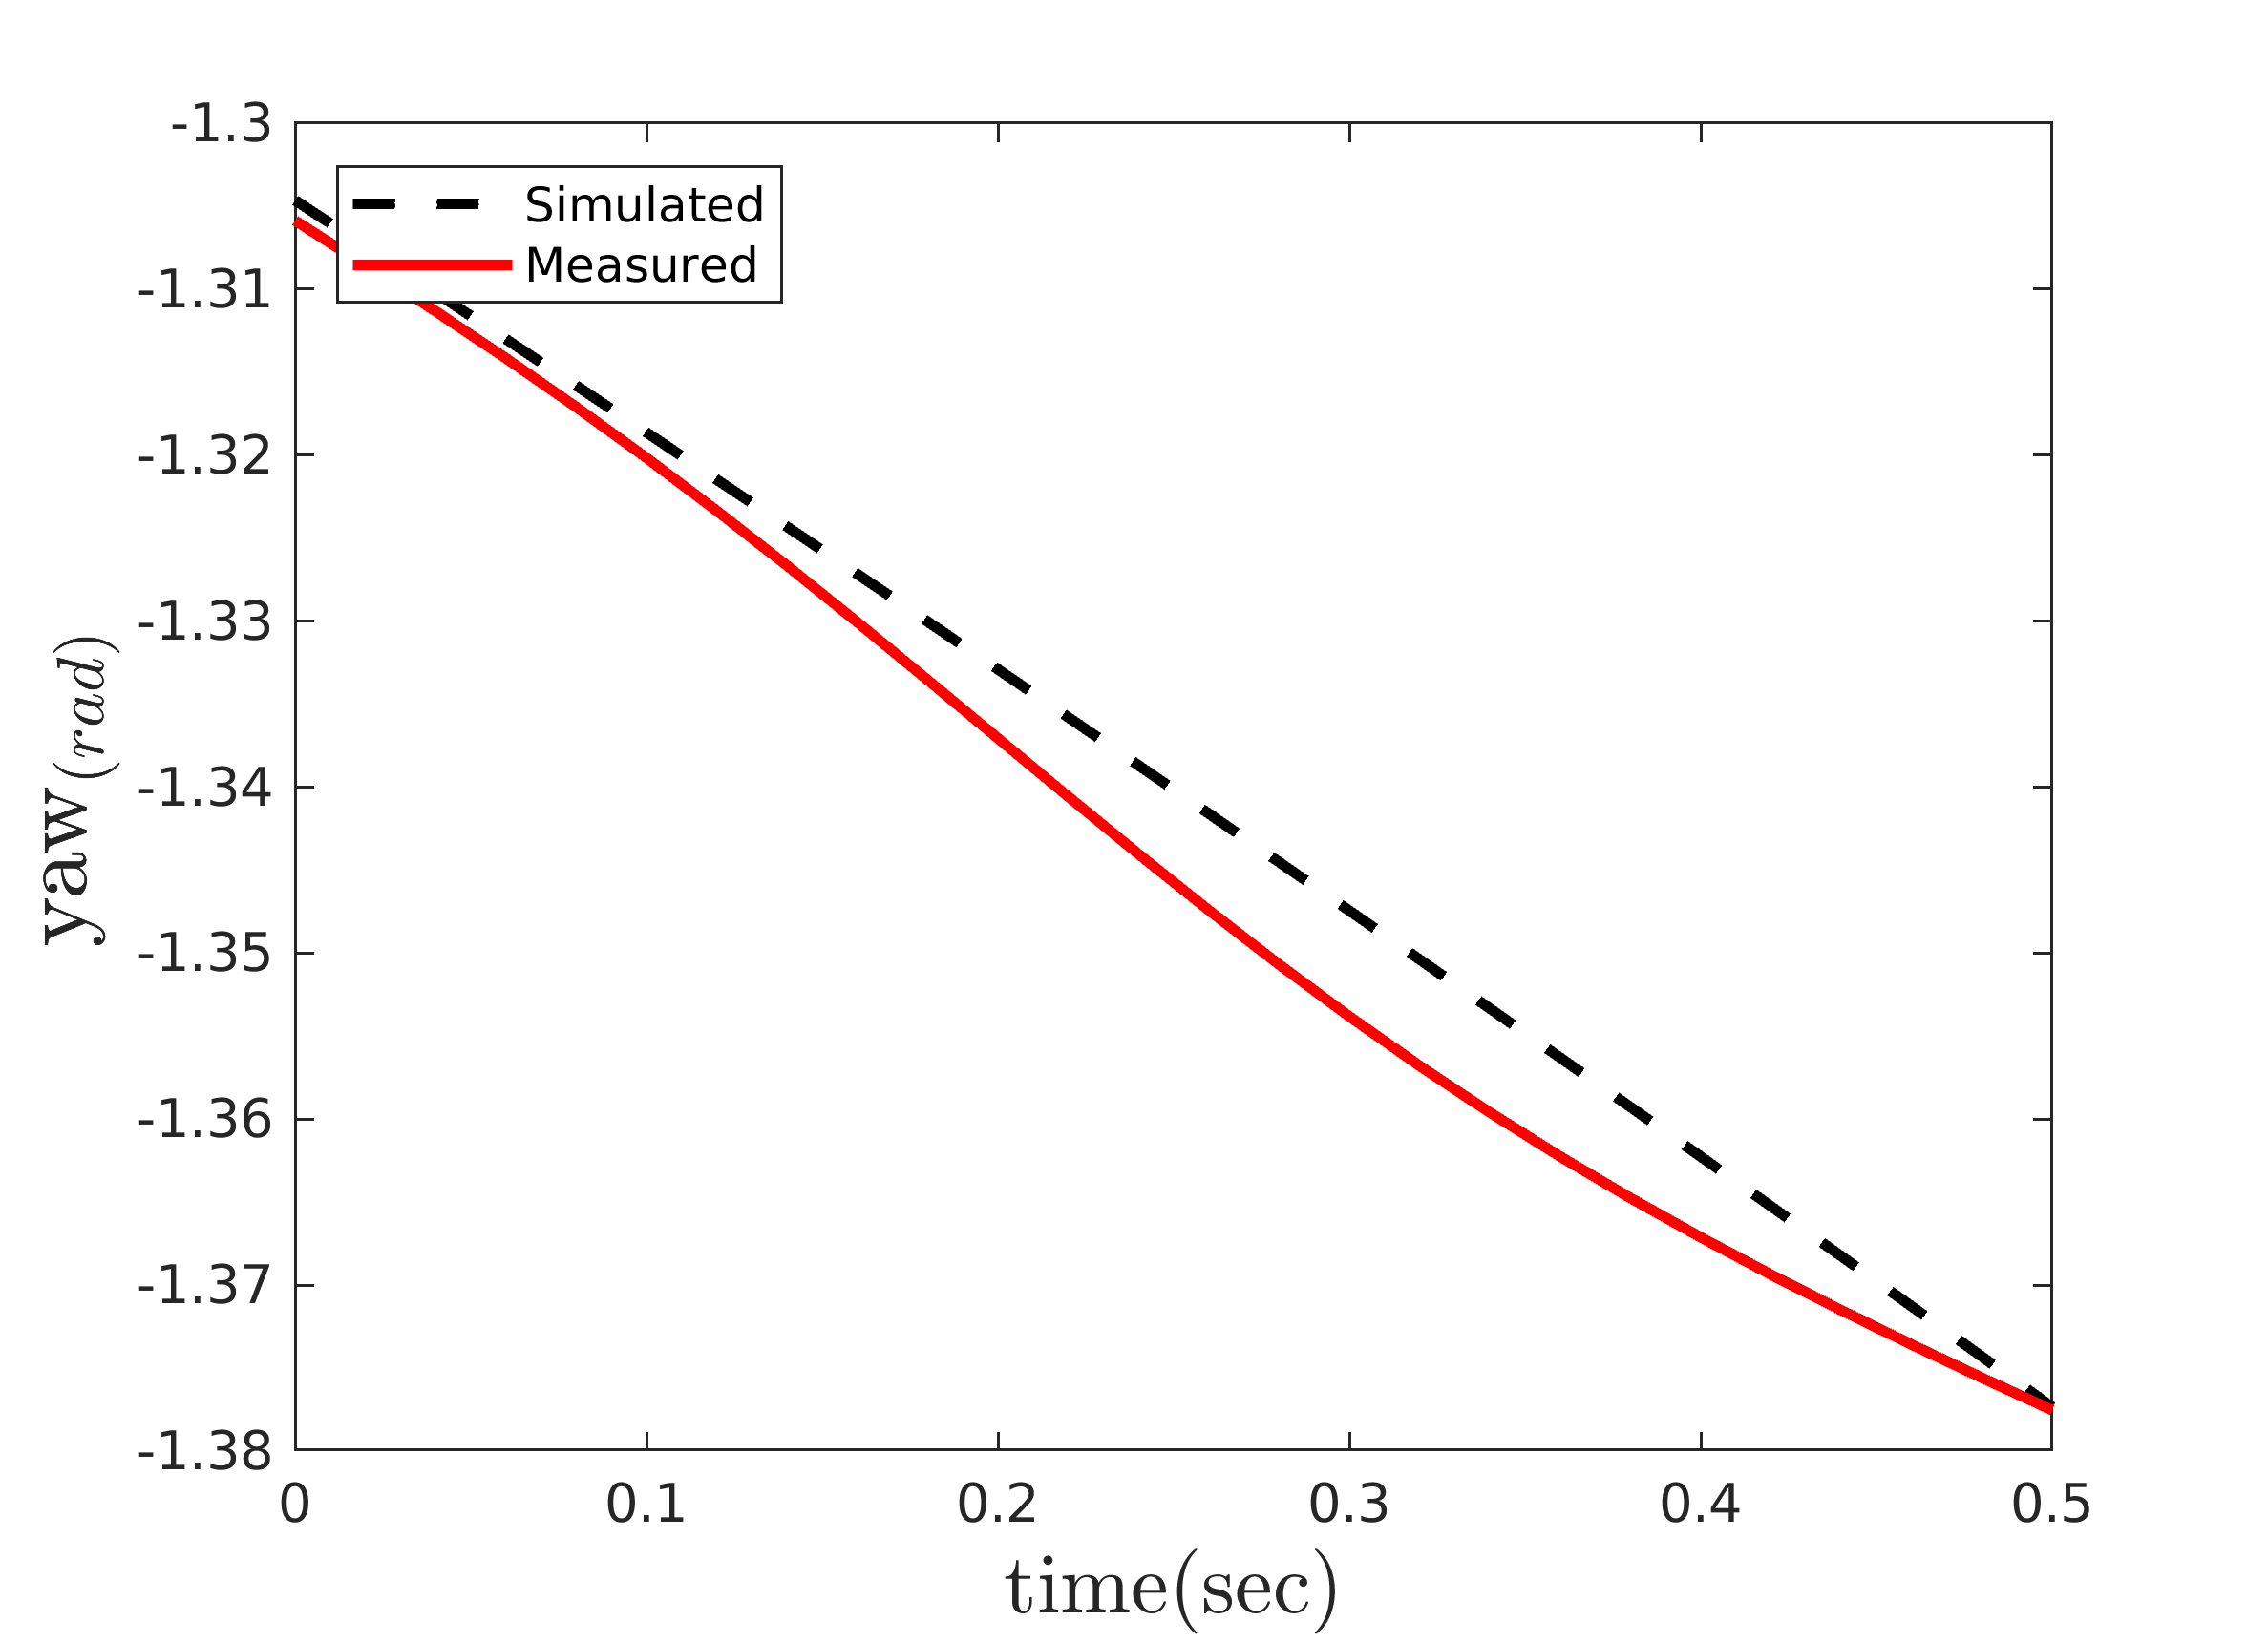
\includegraphics[width=2.3in]{../Figures/RCP/yaw_parameter_estimation/RCP_yaw_S2.png}
% 	\label{fig: yaw PE}}
% 	\caption{Simulation results for the network.} \label{fig_sim}
% \end{figure*}





\section{Differential Game}\label{sec: diff game}
Differential games are a series of problems that arise while examining and simulating dynamic systems in game theory.
%  A differential game is a game in which the player who is trying to maximize the utility of his strategy is the opponent. The player who is trying to minimize the utility of his strategy is the player who is trying to maximize the utility of the opponent's strategy.
% In the context of differential games, differential games in game theory address the modeling and analysis of dynamic systems.
% Differential games are a class of games in which the players are able to model the system and the players are able to choose the optimal move.
% Differential games are sets of issues that arise while examining and simulating dynamic systems in game theory.
Differential equations
%  are used to 
 simulate how a state variable or set of state variables changes over time.
% Differential equations are used to model the evolution over time of a state variable or variables.
\subsection{Differential Game Usage in a Quadrotor Control Loop}
This paper describes the state of two players in different loop control of a quadrotor.
% It is considered that two players are involved in this research.
% In this paper, there are considered to be two players.
Three groups of players are identified: two players for roll loop control, two players for pitch loop control, and two players for yaw loop control.
% Two players associated with roll loop control, two players associated with pitch loop control, and two players associated with yaw loop control are defined.
% The space states of a continuous linear system are shown below.
% The space state of roll, pitch, and yaw are defined below.
%% fix i to italic
% \begin{equation}\label{system_dynamic}
%     \begin{split}
%              &\boldsymbol{\dot{\mathrm{x_i}}}(t) = \boldsymbol{\mathrm{A_ix_i}}(t) + \boldsymbol{\mathrm{B_iu_i}}(t) + \boldsymbol{\mathrm{B_{i_d}u_{i_d}}}(t)%, \quad \boldsymbol{x}(0) = \boldsymbol{x}_0
%         \\
%         &\boldsymbol{\mathrm{y_i}}(t) = \boldsymbol{\mathrm{C_ix_i}}(t) + \boldsymbol{\mathrm{D_iu_i}}(t) + \boldsymbol{\mathrm{D_{i_d}u_{i_d}}}(t)\\
% 		& i =1, 2, 3
% 		%  \text{Roll, Pitch, Yaw}
%     \end{split}
% \end{equation}
% Where $\boldsymbol{\mathrm{x}}$ is the vector of the state variables, $\boldsymbol{\dot{\mathrm{x}}}$ is the time derivative of the state vector, $\boldsymbol{\mathrm{u}}$ is the controller input vector, $\boldsymbol{\mathrm{u_d}}$ is the disturbance input vector, $\boldsymbol{\mathrm{y}}$ is the output vector, $\boldsymbol{\mathrm{A}}$ is the state matrix, $\boldsymbol{\mathrm{B}}$ is the controller input matrix, $\boldsymbol{\mathrm{B_d}}$ is the disturbance input matrix,
% $\boldsymbol{\mathrm{C}}$ is the output matrix, $\boldsymbol{\mathrm{D}}$ is controller the output matrix and $\boldsymbol{\mathrm{D_d}}$ is disturbance the output matrix.
% Equation \eqref{system_dynamic} demonstrates how both participants have an impact on the quadrotor's dynamics.
% As shown in equation 1, both players affect the dynamics of the system.
The second player may progress toward the goal as a result of the first player's exertion, or vice versa.
% The first player's effort could push the second player away from the goal, or the other way around.
This paper considers the case that players do not cooperate in order to realize their goals.
% The situation where players do not work together (non-cooperative) to achieve their objectives is examined in the paper.
% The paper examines the situation in which players do not cooperate to achieve their goals.
In this case, every player knows at time $t \in [0, T]$ just the initial state $\boldsymbol{\mathrm{x}_0}$ and the model structure.
% This scenario can be interpreted as the players simultaneously determining their actions, next submitting their actions. 
% The players can be interpreted as simultaneously determining their actions, then submitting them.
For the game between two players in each loop control, the set of Nash equilibria is used. Formal Nash equilibrium is defined as follows.
% Here are the formal Nash equilibrium definitions for games (1) and (2).
% defenition
An admissible set of actions $(\boldsymbol{u_1}^*,  \boldsymbol{u_{i_d}}^*)$ is a Nash equilibrium for the game between two player in each loop control; if for all admissible $(\boldsymbol{u_i},  \boldsymbol{u_{i_d}})$, the following inequalities hold:
\begin{equation}\label{nash_lqe}
	J_1(\boldsymbol{\mathrm{u_i}}^*, \boldsymbol{\mathrm{u_{i_d}}}^*)\leq J_1(\boldsymbol{\mathrm{u_1}}, \boldsymbol{\mathrm{u_{i_d}}}^*) \text{\rm{ , }}
	J_2(\boldsymbol{\mathrm{u_i}}^*, \boldsymbol{\mathrm{u_{i_d}}}^*)\leq 
	J_2(\boldsymbol{\mathrm{u_i}}^*, \boldsymbol{\mathrm{u_{i_d}}})
\end{equation}
% Here admissibility is meant in the sense that $\boldsymbol{\mathrm{u_i}}(.)$ belongs to some restricted set, where this set depends on the information players have on the game, the set of strategies the players like to use to control the system, and the system (2) must have a unique solution.
% The term admissibility refers to the fact that u(.) belongs to a restricted set determined by the information players have about the game, the strategies they use to control the system, and the uniqueness of the solution.
\subsection{LQDG controller}
% For the each control loop described in equation \eqref{system_dynamic}, 
LQDG optimum control effort calculates from equation \eqref{LQDG_u}.
% The optimum control effort calculated by LQDG for the system described in equation 1 is calculated using equation 2.
% For the system described in equation 1, LQDG optimum control effort calculates from equation 2.
\begin{equation}\label{LQDG_u}
	\boldsymbol{\mathrm{u_i}}(t) = -\boldsymbol{\mathrm{R_{i}}}^{-1}\boldsymbol{\mathrm{B_i}}^\mathrm{T}\boldsymbol{\mathrm{P_{i}}}(t)\boldsymbol{\mathrm{x}}(t) = -\boldsymbol{\mathrm{K_{i}}}(t)\boldsymbol{\mathrm{x}}(t),\quad i = 1, 2, 3
\end{equation}
In equation \eqref{LQDG_u}, $\boldsymbol{\mathrm{K_{i}}}$ is the optimal feedback gain. Assuming that the other players will make their worst move, this gain is calculated to minimize the quadratic cost function equation \eqref{cost} of controller player for each control loop of quadrotor.
\begin{equation}\label{cost}
    \begin{split}
        J_i( \boldsymbol{\mathrm{u_i}},  \boldsymbol{\mathrm{u_{i_d}}}) = \int_{0}^{T}\biggl (&\boldsymbol{\mathrm{x_i}} ^\mathrm{T}(t) \boldsymbol{\mathrm{Q_i}} \boldsymbol{\mathrm{x_i}}(t)+
        \boldsymbol{\mathrm{u_i}} ^\mathrm{T}(t) \boldsymbol{\mathrm{R_{i}}} \boldsymbol{\mathrm{u_i}}(t)-\\
        &\boldsymbol{\mathrm{u_{i_d}}} ^\mathrm{T}(t)\boldsymbol{\mathrm{ R_{i_d} u_{i_d}}}(t)
        \biggl )\mathrm{d}t, \quad i = 1, 2, 3 
    \end{split} 
\end{equation}
Here the matrices $\boldsymbol{\mathrm{Q_i}}$ and  $\boldsymbol{\mathrm{R_{i}}}$ are assumed to be symmetric and $\boldsymbol{\mathrm{R_{i}}}$ positive definite.
$\boldsymbol{\mathrm{P_{i}}}$ is found by solving the continuous time couple Riccati differential equation:
\begin{equation}\label{coupled_riccatti_LQDG}
    \begin{split}
        &\begin{split}
             \boldsymbol{\dot{\mathrm{P}}_i}(t) = -&\boldsymbol{\mathrm{A_i}}^\mathrm{T}\boldsymbol{\mathrm{P_i}}(t) - \boldsymbol{\mathrm{P_i}}(t)\boldsymbol{\mathrm{A_i}} - \boldsymbol{\mathrm{Q_i}} +\boldsymbol{\mathrm{P_i}}(t)\boldsymbol{\mathrm{S_i}}(t)\boldsymbol{\mathrm{P_i}}(t) +\\ &\boldsymbol{\mathrm{P_i}}(t)\boldsymbol{\mathrm{S_{i_d}}}(t)\boldsymbol{\mathrm{P_{i_d}}}(t)
        \end{split}\\
        &\begin{split}
            \boldsymbol{\dot{\mathrm{P}}_{i_d}}(t) = -&\boldsymbol{\mathrm{A_i}}^\mathrm{T}\boldsymbol{\mathrm{P_{i_d}}}(t) - \boldsymbol{\mathrm{P_{i_d}}}(t)\boldsymbol{\mathrm{A_i}} - \boldsymbol{\mathrm{Q_{i_d}}} +\\ & \boldsymbol{\mathrm{P_{i_d}}}(t)\boldsymbol{\mathrm{S_{i_d}}}(t)\boldsymbol{\mathrm{P_{i_d}}}(t) +\boldsymbol{\mathrm{P_{i_d}}}(t)\boldsymbol{\mathrm{S_i}}(t)\boldsymbol{\mathrm{P_i}}(t)
        \end{split}
    \end{split}
\end{equation}
Using the shorthand notation $\boldsymbol{S_i} := \boldsymbol{B_iR_{i}}^{-1}\boldsymbol{B_i}^\mathrm{T}$. %?????????????????????


\subsection{LQIDG controller}
The absence of an integrator in the LQDG controller may result in steady-state errors due to disturbances or modeling errors.
% The LQDG controller's lack of an integrator could lead to steady-state errors due to disturbances or faulty modeling.
The LQIDG controller is based on the LQDG controller to eliminate this error.

The LQIDG controller adds the integral of the difference between the system output and the desired value to the state vector.
% In this controller, the integral of the difference between the system output and the desired value is added to the state vector.
% The integral of the difference between the system output and the desired value is added to the state vector by the LQIDG controller.
Therefore, The augmented space states of a continuous linear system are shown below.
\begin{equation}\label{lqidg_x}
    \boldsymbol{\mathrm{x_a}} = \begin{bmatrix}
        \boldsymbol{\mathrm{x_d}} - \boldsymbol{\mathrm{x}}\\
        \displaystyle \int (\boldsymbol{\mathrm{z_d}} - \boldsymbol{\mathrm{z}})
    \end{bmatrix}
\end{equation}
Where $\boldsymbol{\mathrm{x_a}}$ is the vector of augmented state variables, $\boldsymbol{\mathrm{x_d}}$ is the vector of the desired state variables, and $\boldsymbol{\mathrm{y_d}}$ is the desired output vector.
As a result, the state vector and the output vector are equal.
% Hence, the output vector equals the state vector.
\begin{equation}
	\boldsymbol{\mathrm{z}} = \boldsymbol{\mathrm{x}}
\end{equation}
The following represents the system dynamics in the augmented state space.
% Following is a representation of the system dynamics in the augmented state space.
% In the augmented state space, the system's dynamics are shown below.
\begin{equation}\label{systemlqidg}
	\begin{split}
		\boldsymbol{\dot{\mathrm{x}}_a}(t) &= \boldsymbol{\mathrm{A_ax_a}}(t) + \boldsymbol{\mathrm{B_{{a_1}}u_{a_1}}}(t) + \boldsymbol{\mathrm{B_{{a_2}}u_{a_2}}}(t)%, \quad \boldsymbol{x}(0) = \boldsymbol{x}_0%
		% \\
		% \boldsymbol{\mathrm{y}}(t) &= \boldsymbol{\mathrm{C_ax_a}}(t) + \boldsymbol{\mathrm{D_{{a_1}}u_{a_1}}}(t) + \boldsymbol{\mathrm{D_{{a_2}}u_{a_2}}}(t)
	\end{split}
\end{equation}
Where matrices $\boldsymbol{\mathrm{A_a}}$ and $\boldsymbol{\mathrm{B_a}}$ are defined as follows:
\begin{equation}
	\boldsymbol{\mathrm{A_a}} = \begin{bmatrix}
		\boldsymbol{\mathrm{A}} &0\\
		\boldsymbol{\mathrm{C}} & 0
	\end{bmatrix}
, \quad
	\boldsymbol{\mathrm{B_a}} = \begin{bmatrix}
		\boldsymbol{\mathrm{B}}\\
		0
	\end{bmatrix}
\end{equation}
By introducing a new space state for the system, the remaining design phases of the LQIDG controller are comparable to those of the LQDG controller. LQIDG optimum control effort calculates from equation \eqref{LQIDG_u}.
\begin{equation}\label{LQIDG_u}
	\begin{split}
		\boldsymbol{\mathrm{u_i}}(t) &= -\boldsymbol{\mathrm{R_{ii}}}^{-1}\boldsymbol{\mathrm{B_{a_i}}}^\mathrm{T}\boldsymbol{\mathrm{P_{a_i}}}(t)\boldsymbol{\mathrm{x_a}}(t) \\
		\boldsymbol{\mathrm{u_i}}(t) &= - \boldsymbol{\mathrm{K_{a_i}}}(t)\boldsymbol{\mathrm{x_a}}(t),~ i = 1, 2, 3
	\end{split}
\end{equation}





In equation \eqref{LQIDG_u}, $\boldsymbol{\mathrm{K_{a_i}}}$ is the optimal feedback gain. Assuming that the other players will make their worst move, this gain is calculated to minimize the quadratic cost function, equation \eqref{cost_LQIDG}, of player number i.
\begin{equation}\label{cost_LQIDG}
    \begin{split}
        J_i( \boldsymbol{\mathrm{u_i}},  \boldsymbol{\mathrm{u_{i_d}}}) = \int_{0}^{T}\biggl (\boldsymbol{\mathrm{x_a}} ^\mathrm{T}(t) \boldsymbol{\mathrm{Q_i}} \boldsymbol{\mathrm{x_a}}(t)+
        &\boldsymbol{\mathrm{u_i}} ^\mathrm{T}(t) \boldsymbol{\mathrm{R_{i}}} \boldsymbol{\mathrm{u_i}}(t)-\\
        &\boldsymbol{\mathrm{u_{i_d}}} ^\mathrm{T}(t)\boldsymbol{\mathrm{ R_{i_d} u_{i_d}}}(t)
        \biggl )\mathrm{d}t
    \end{split} 
\end{equation}
$\boldsymbol{\dot{\mathrm{P}}_{a_i}}$ is found by solving the continuous time couple Riccati differential equation:
\begin{equation}\label{coupled_riccatti_LQIDG}
    \begin{split}
        &\begin{split}
            \boldsymbol{\dot{\mathrm{P}}_{a_i}}(t) = -&\boldsymbol{\mathrm{A_a}}^\mathrm{T}\boldsymbol{\mathrm{P_{a_i}}}(t) - \boldsymbol{\mathrm{P_{a_i}}}(t)\boldsymbol{\mathrm{A_a}} - \boldsymbol{\mathrm{Q_i}} +\\ &\boldsymbol{\mathrm{P_{a_i}}}(t)\boldsymbol{\mathrm{S_{a_i}}}(t)\boldsymbol{\mathrm{P_{a_i}}}(t) + \boldsymbol{\mathrm{P_{a_i}}}(t)\boldsymbol{\mathrm{S_{a_{i_d}}}}(t)\boldsymbol{\mathrm{P_{a_{i_d}}}}(t)
        \end{split}\\
        &\begin{split}
            \boldsymbol{\dot{\mathrm{P}}_{a_{i_d}}}(t) = -&\boldsymbol{\mathrm{A_a}}^\mathrm{T}\boldsymbol{\mathrm{P_{a_{i_d}}}}(t) - \boldsymbol{\mathrm{P_{a_{i_d}}}}(t)\boldsymbol{\mathrm{A_a}} - \boldsymbol{\mathrm{Q_{i_d}}} +\\ &\boldsymbol{\mathrm{P_{a_{i_d}}}}(t)\boldsymbol{\mathrm{S_{a_{i_d}}}}(t)\boldsymbol{\mathrm{P_{a_{i_d}}}}(t) + \boldsymbol{\mathrm{P_{a_{i_d}}}}(t)\boldsymbol{\mathrm{S_{a_i}}}(t)\boldsymbol{\mathrm{P_{a_i}}}(t)
        \end{split}
    \end{split}
\end{equation}
Using the shorthand notation $\boldsymbol{S_{a_i}} := \boldsymbol{B_{a_i}R_{i}}^{-1}\boldsymbol{B_{a_i}}^\mathrm{T}$. 

%?????????????????????




% \section{Simulation}




% In this section, the quadrotor roll loop control is simulated in the presence of LQR, LQDG, and LQIDG controllers. Then, the simulation of two and three degrees of freedom was done in the presence of the LQIDG controller.
% \subsection{Roll Loop Control}

% LQR weighting matrices are optimized using the TCACS optimization method in the simulation.
% % In the simulation, the TCACS optimization method is used to optimize the LQR weighting matrices.
% ITSE is considered for the TCACS input cost function.
% % TCACS input cost function is considered as ITSE.
% Here are the weighting matrices for the optimized output.
% % The weighting matrices of the optimized output are given below.
% \begin{equation}
% 	\boldsymbol{\mathrm{Q}}_{\text{LQR}} = \begin{bmatrix}
% 		0.5215 & 0\\
% 		0 & 0.0745
% 	\end{bmatrix}, \quad R_{\text{LQR}} =  0.0001
% \end{equation} 

% % \subsection{LQDG}
% The weighting matrices used in the LQDG portion are chosen like that of the LOR.
% % LQDG weighting matrices are chosen like the method used in the LQR section.
% % In the LQDG section, weighting matrices are selected similarly to those used in the LOR section.
% \begin{equation}
% 	\boldsymbol{\mathrm{Q}}_{\text{LQDG}} = \begin{bmatrix}
% 		100 & 0\\
% 		0 & 0.078
% 	\end{bmatrix}, \quad R_{{\text{LQDG}}} =  1, \quad R_{d_{_\text{LQDG}}} =  99.96
% \end{equation}

% % \begin{equation}
% % 	\boldsymbol{\dot{\mathrm{P}}_{1}} = \begin{bmatrix}
		
% % 		286.0470  & 39.1188\\
% % 		39.1188   & 8.8510\\
% %     \end{bmatrix}    
% % \end{equation}

% \begin{equation}
%     \boldsymbol{\mathrm{K_{1}}} = \begin{bmatrix}
%         39.1188   & 8.8510
%     \end{bmatrix}
% \end{equation}

% % \subsection{LQIDG}
% LQIDG weighting matrices are chosen like the method used in the LQR and LQDG sections.
% \begin{equation}
%     \begin{split}
%         &\boldsymbol{\mathrm{Q_{{\text{LQIDG}}}}} = \begin{bmatrix}
%             0.1707 &0& 0& 0\\
%             0 &  0.12 & 0 &0 \\
%             0 & 0 & 837.8606 & 0\\
%             0 & 0 & 0 & 756.1341
%         \end{bmatrix}
%         \\[1em]
%         &R_{{\text{LQIDG}}} =  1, \quad R_{d_{_\text{LQIDG}}} =  7.7422
%     \end{split}
% \end{equation}

% % \begin{equation}
% % 	\boldsymbol{\dot{\mathrm{P}}_{a_1}} = \begin{bmatrix}
% % 		10924.84&   39.83 & 1014.34 & -10629.93\\
% % 		39.83   &  8.40 & 27.22& 11.70\\
% % 		1014.34 &  27.22 & 1047.80 & -756.13\\
% % 		-10658.93 & 11.70 & -756.13 & 10658.93
% % 	\end{bmatrix}
% % \end{equation}
% \begin{equation}
% 	\boldsymbol{\mathrm{K_{a_1}}} = \begin{bmatrix}
% 		28.1410 &   8.4017  & 27.2223  & 11.6894
% 	\end{bmatrix}
% \end{equation}
% \subsection{Roll-Pitch Loop Control}
% \begin{equation}
% 	\begin{split}
% 		\boldsymbol{\mathrm{Q}}_{{\text{LQIDG}_{\text{roll}}}} &= \begin{bmatrix}
% 			585.9 &0& 0& 0\\
% 			0 &  31.1 & 0 &0 \\
% 			0 & 0 & 83.8 & 0\\
% 			0 & 0 & 0 & 0
% 		\end{bmatrix}\\[1em]
% 	    \boldsymbol{\mathrm{Q}}_{{\text{LQIDG}_{\text{pitch}}}} &= \begin{bmatrix}
% 		546.5 &0& 0& 0\\
% 		0 &  311.4 & 0 &0 \\
% 		0 & 0 & 2.22 & 0\\
% 		0 & 0 & 0 & 0
% 		\end{bmatrix}\\[1em]
% 	 R_{{\text{LQIDG}}} &=  1, \quad R_{d_{\text{LQIDG}}} =  7.7422
% 	\end{split}
% \end{equation}

% \subsection{Roll-Pitch-Yaw Loop Control}
% \begin{equation}
% 	\begin{split}
% 		\boldsymbol{\mathrm{Q}}_{{\text{LQIDG}_{\text{roll}}}} &= \begin{bmatrix}
% 			631.85 & 0 & 0 & 0  \\ 
% 			0 & 214.28 & 0 & 0  \\ 
% 			0 & 0 & 7.91 & 0  \\ 
% 			0 & 0 & 0 & 0.01  \\ 
% 		\end{bmatrix} \\[1em]
% 		\boldsymbol{\mathrm{Q}}_{{\text{LQIDG}_{\text{pitch}}}} &= \begin{bmatrix}
% 			0.01 & 0 & 0 & 0  \\
% 			0 & 873.93 & 0 & 0  \\ 
% 			0 & 0 & 9853.09 & 0 \\ 
% 			0 & 0 & 0 & 0.12  \\ 
% 		\end{bmatrix}\\[1em]
% 		\boldsymbol{\mathrm{Q}}_{{\text{LQIDG}_{\text{yaw}}}}  &= \begin{bmatrix}
% 			0.03 & 0 & 0 & 0 \\ 
% 			0 & 0.17 & 0 & 0 \\ 
% 			0 & 0 & 1.81 & 0 \\ 
% 			0 & 0 & 0 & 0.45 \\
% 		\end{bmatrix}\times 10^{-4}\\[1em]
%           R_{{\text{LQIDG}}} &= 1, \quad  R_{d_{\text{LQIDG}}} = 1.2577
% 	\end{split}
% \end{equation}

\section{Result and Discussion}\label{sec:results}


Here, the results of the LQIR-DG controller method are devoted to the control loops of the roll, pitch, and yaw of the experimental setup of the quadrotor. First, the controller parameters are tuned using the results of numerical simulations. Moreover, the performance of the LQIR-DG controller is compared to an LQR control strategy. Estimated parameters are shown in table \ref{tab:parameters}.
\begin{table}[!h]
	\renewcommand{\arraystretch}{1.3}
	\caption{The Estimated Parameter of the Quadrotor}
	\begin{center}
	\begin{tabular}{c c c}
	\hline
	\textbf{Parameter} & \textbf{\textit{Value}}& \textbf{\textit{Units}} \\
	\hline
	$I_{\text{xx}}$ & $0.02839$ & $kg.m^2$ \\
	$I_{yy}$  & $0.03066$ & $kg.m^2$\\
	$I_{zz}$  & $0.0439$ & $kg.m^2$ \\
	$I_{\text{rotor}}$  & $4.4398\times 10^{-5}$ & $kg.m^2$\\
	\hline
	\end{tabular}
	\label{tab:parameters}
	\end{center}
\end{table}
% The LQR controller parameters are presented in Table \ref{table: control gain}.
% \begin{table}[!h]
% 	\renewcommand{\arraystretch}{1.3}
% 	\caption{Parameters of the LQR Controller}
% 	\begin{center}
% 	\begin{tabular}{c c c}
% 	\hline
% 	\textbf{Control Loop} & \textbf{\textit{Initial Value}}& \textbf{\textit{Value After Estimation}} \\
% 	\hline
% 	$A_1$ & $7.312$ & $4.152$ \\
% 	$A_3$  & $1.1\times10^{-4}$ & $5.47\times10^{-5}$\\
% 	$B_1$  & $4.53$ & $4.36$ \\
% 	$B_3$  & $1.1\times10^{-4}$ & $7.13\times10^{-5}$ \\ 
% 	$C_2$  & $5.45\times10^{-5}$ & $1.3\times10^{-5}$ \\
% 	\hline
% 	\end{tabular}
% 	\label{table: control gain}
% 	\end{center}
% \end{table}

\subsection{Performance of the LQIR-DG Controller}

The performance of the LQIR-DG controller is evaluated in Figure 8. The desired and actual outputs, including the roll, pitch, and yaw angles, are compared in \figurename{\ref{fig:result}}. The desired scenario of the simulator is considered a level flight. These figures show that the attitude outputs of the quadrotor converge to the desired values in less than three seconds. Moreover, \figurename{\ref{fig:omega}} show the angular velocity command of the quadrotor, 
respectively. These results illustrate that the LQIR-DG approach appropriately controls the attitude of the experimental setup of the quadrotor. LQIR-DG control weight is described in table \ref{tab:control weight} and $R$ is assumed to be $1$, and $R_d$ is $1.2577$.
\begin{table}[!h]\label{tab:control weight}
	\renewcommand{\arraystretch}{1.3}
	\caption{LQIR-DG Control Parameter}
	\begin{center}
	\begin{tabular}{c c c c c}
	\hline
	\textbf{Control Loop} & \textbf{\textit{$q_1$}}& \textbf{\textit{$q_2$}} 
	& \textbf{\textit{$q_3$}} & \textbf{\textit{$q_4$}} \\
	\hline
	Roll & 
	$631.85$ & $214.28$ & $7.91$ &
	$0.01$ \\
	Pitch & 
	$0.01$ & $873.93$ & $9853.09$ &
	$0.12$ \\
	Yaw & 
	$3e-6$ & $1.7e-5$ & $1.81e-4$ &
	$4.5e-5$ \\
	\hline
	\end{tabular}
	\label{tab2}
	\end{center}
\end{table}


\begin{figure*}[!h]
	\centering
	\subfloat[]{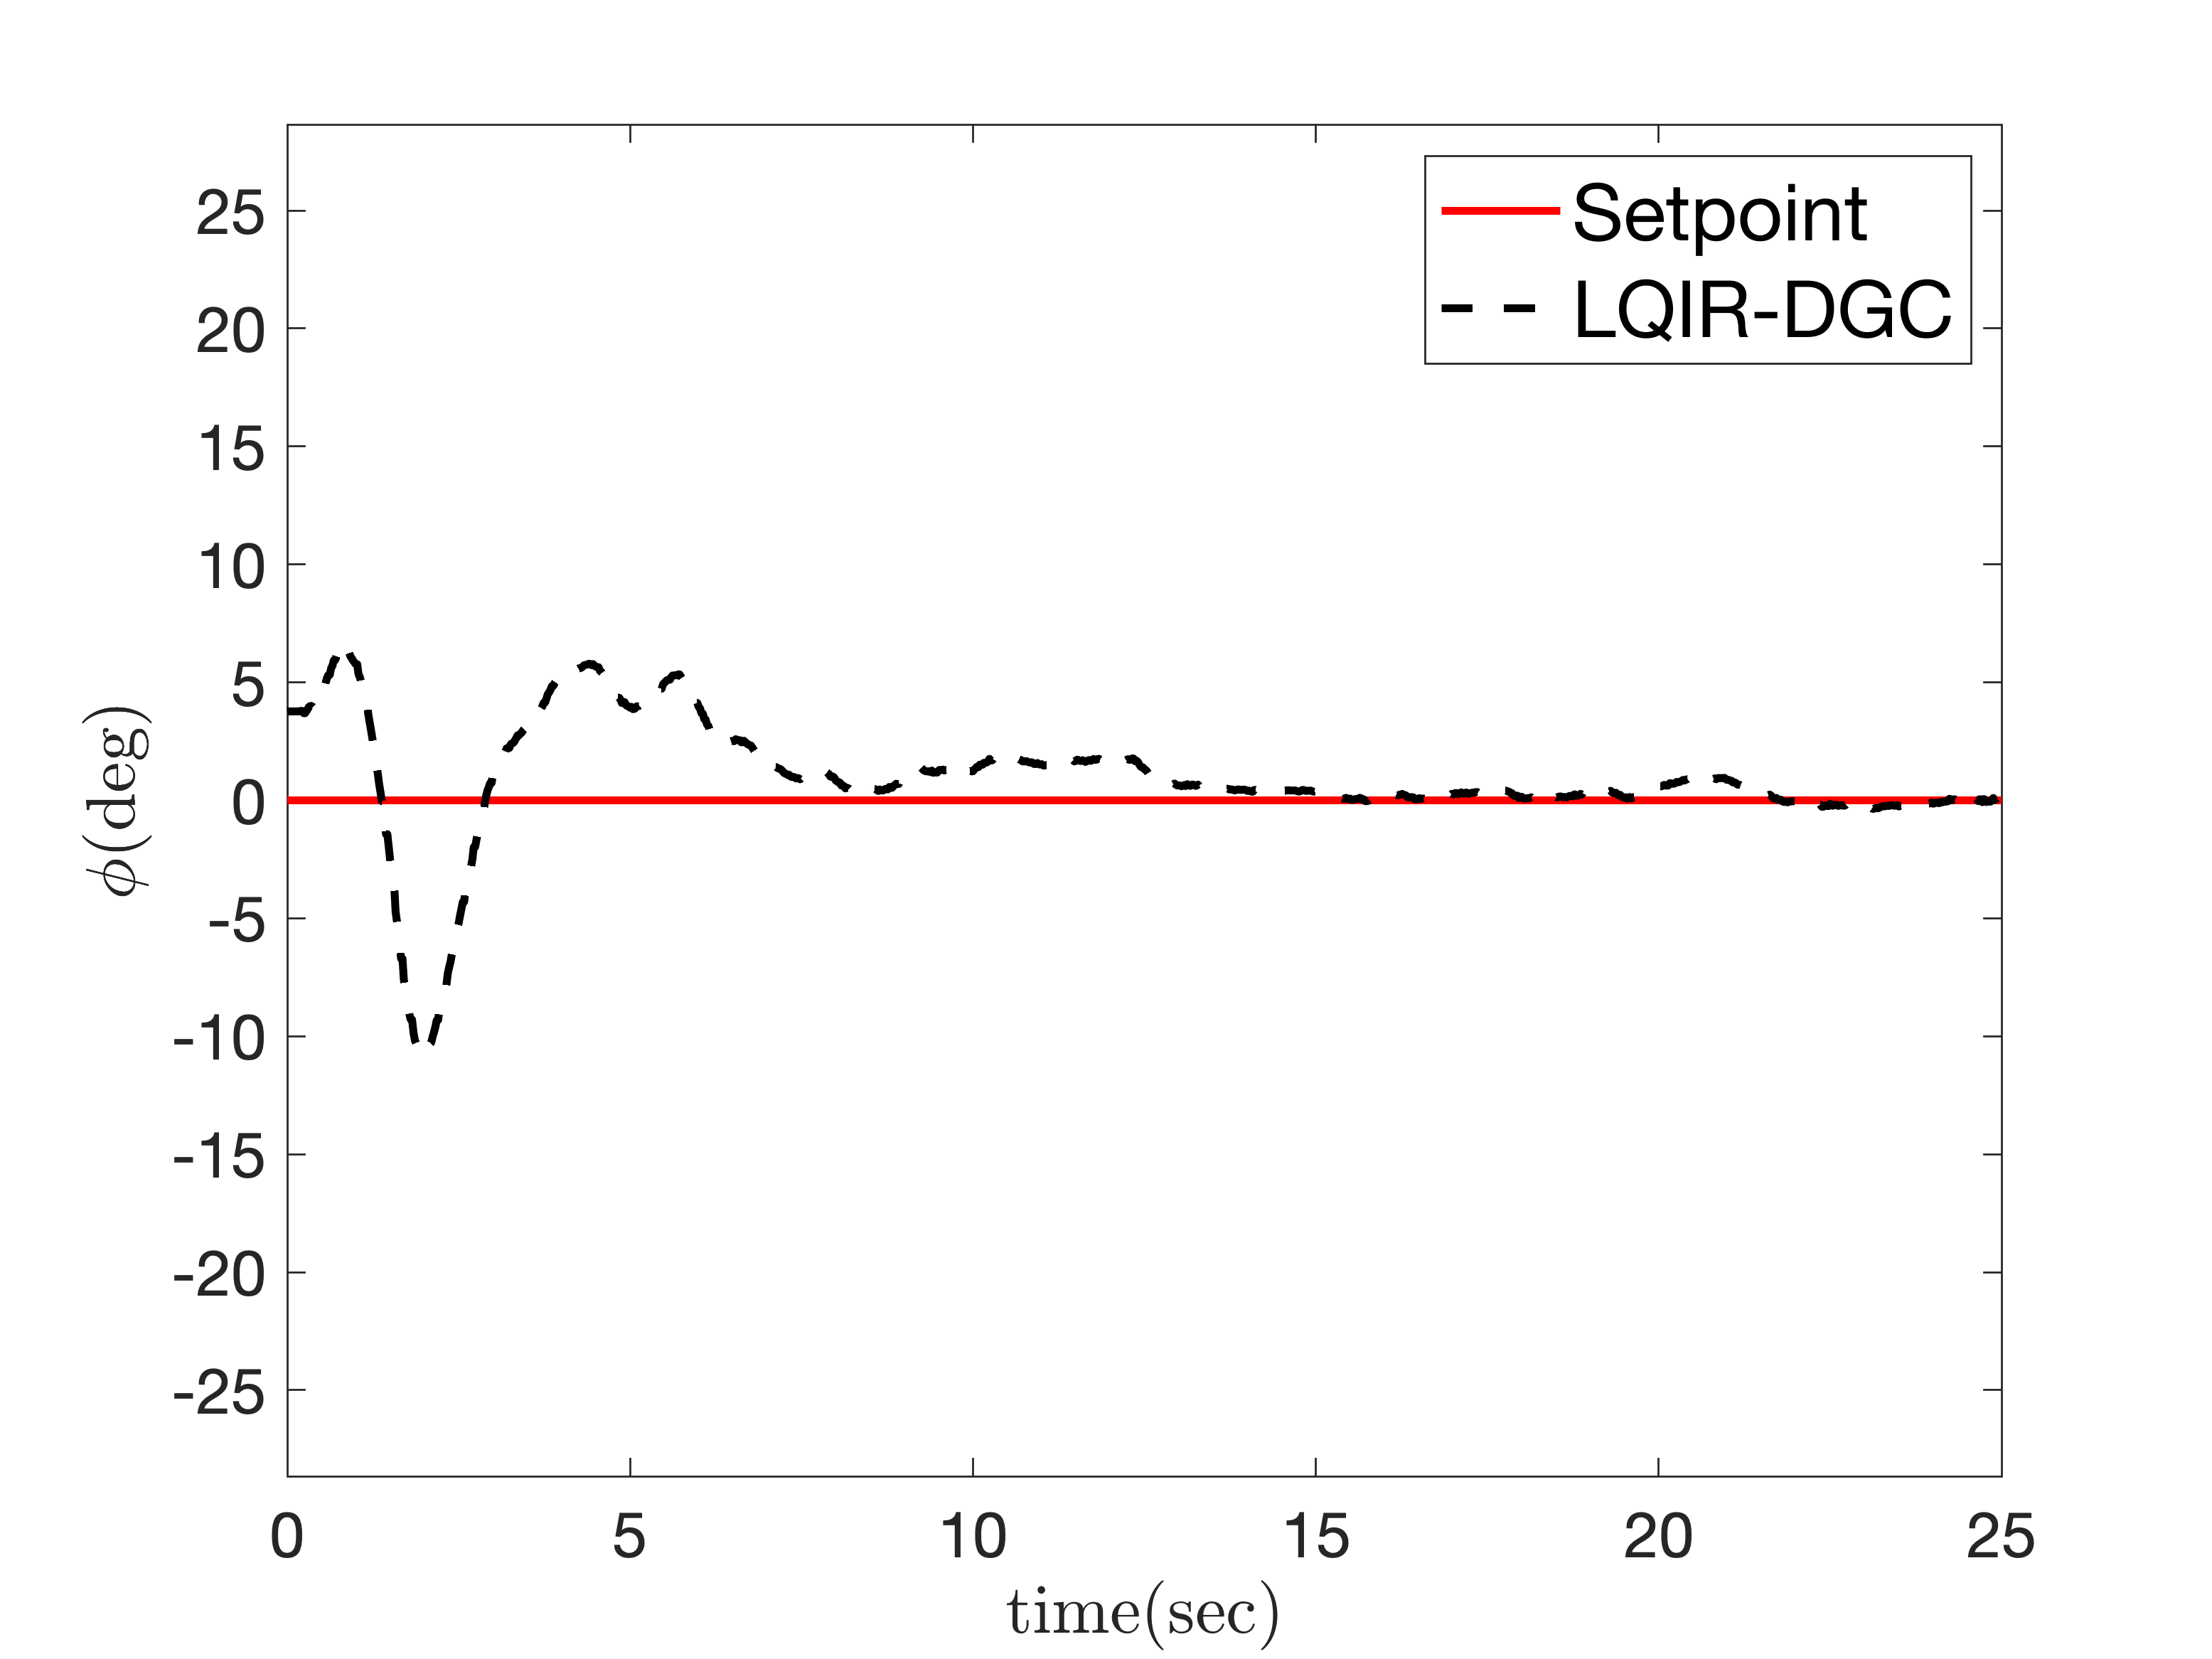
\includegraphics[width=.26\linewidth]{../Figures/Calibration/LQIDG/3DOF/lqidg_roll.png}\label{fig:roll}
	}
	\subfloat[]{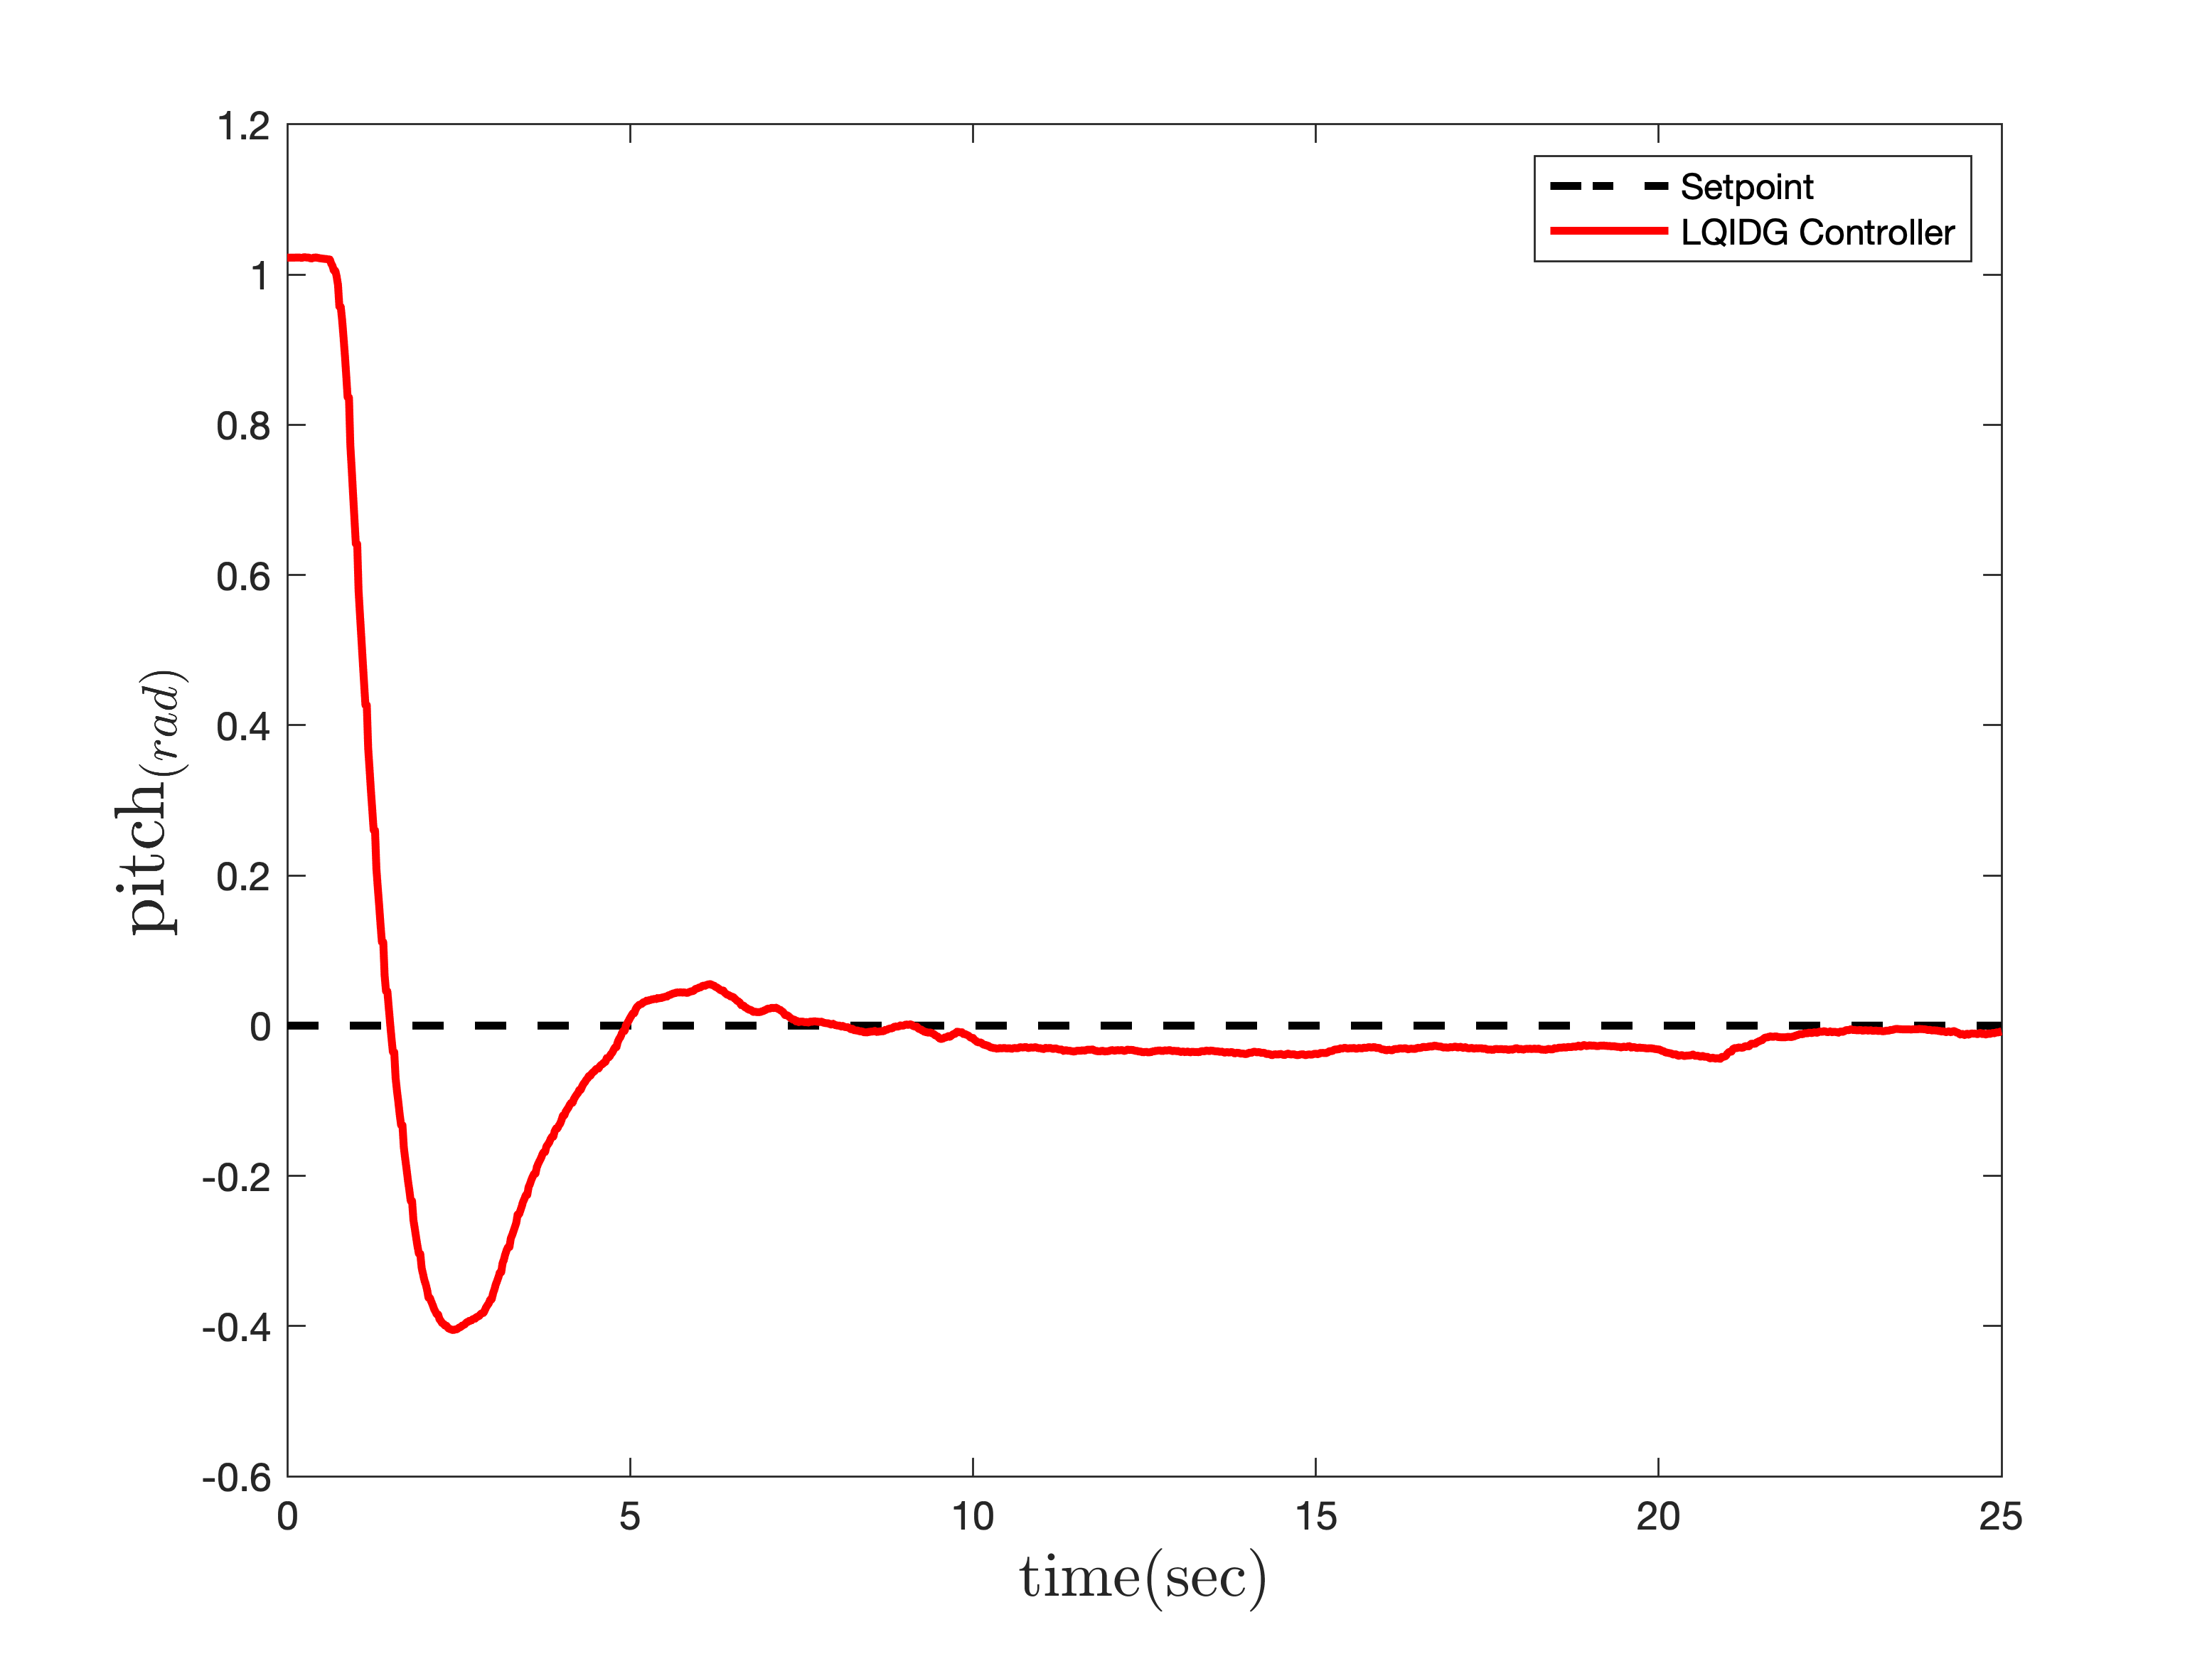
\includegraphics[width=.26\linewidth]{../Figures/Calibration/LQIDG/3DOF/lqidg_pitch.png}
	}
	\subfloat[]{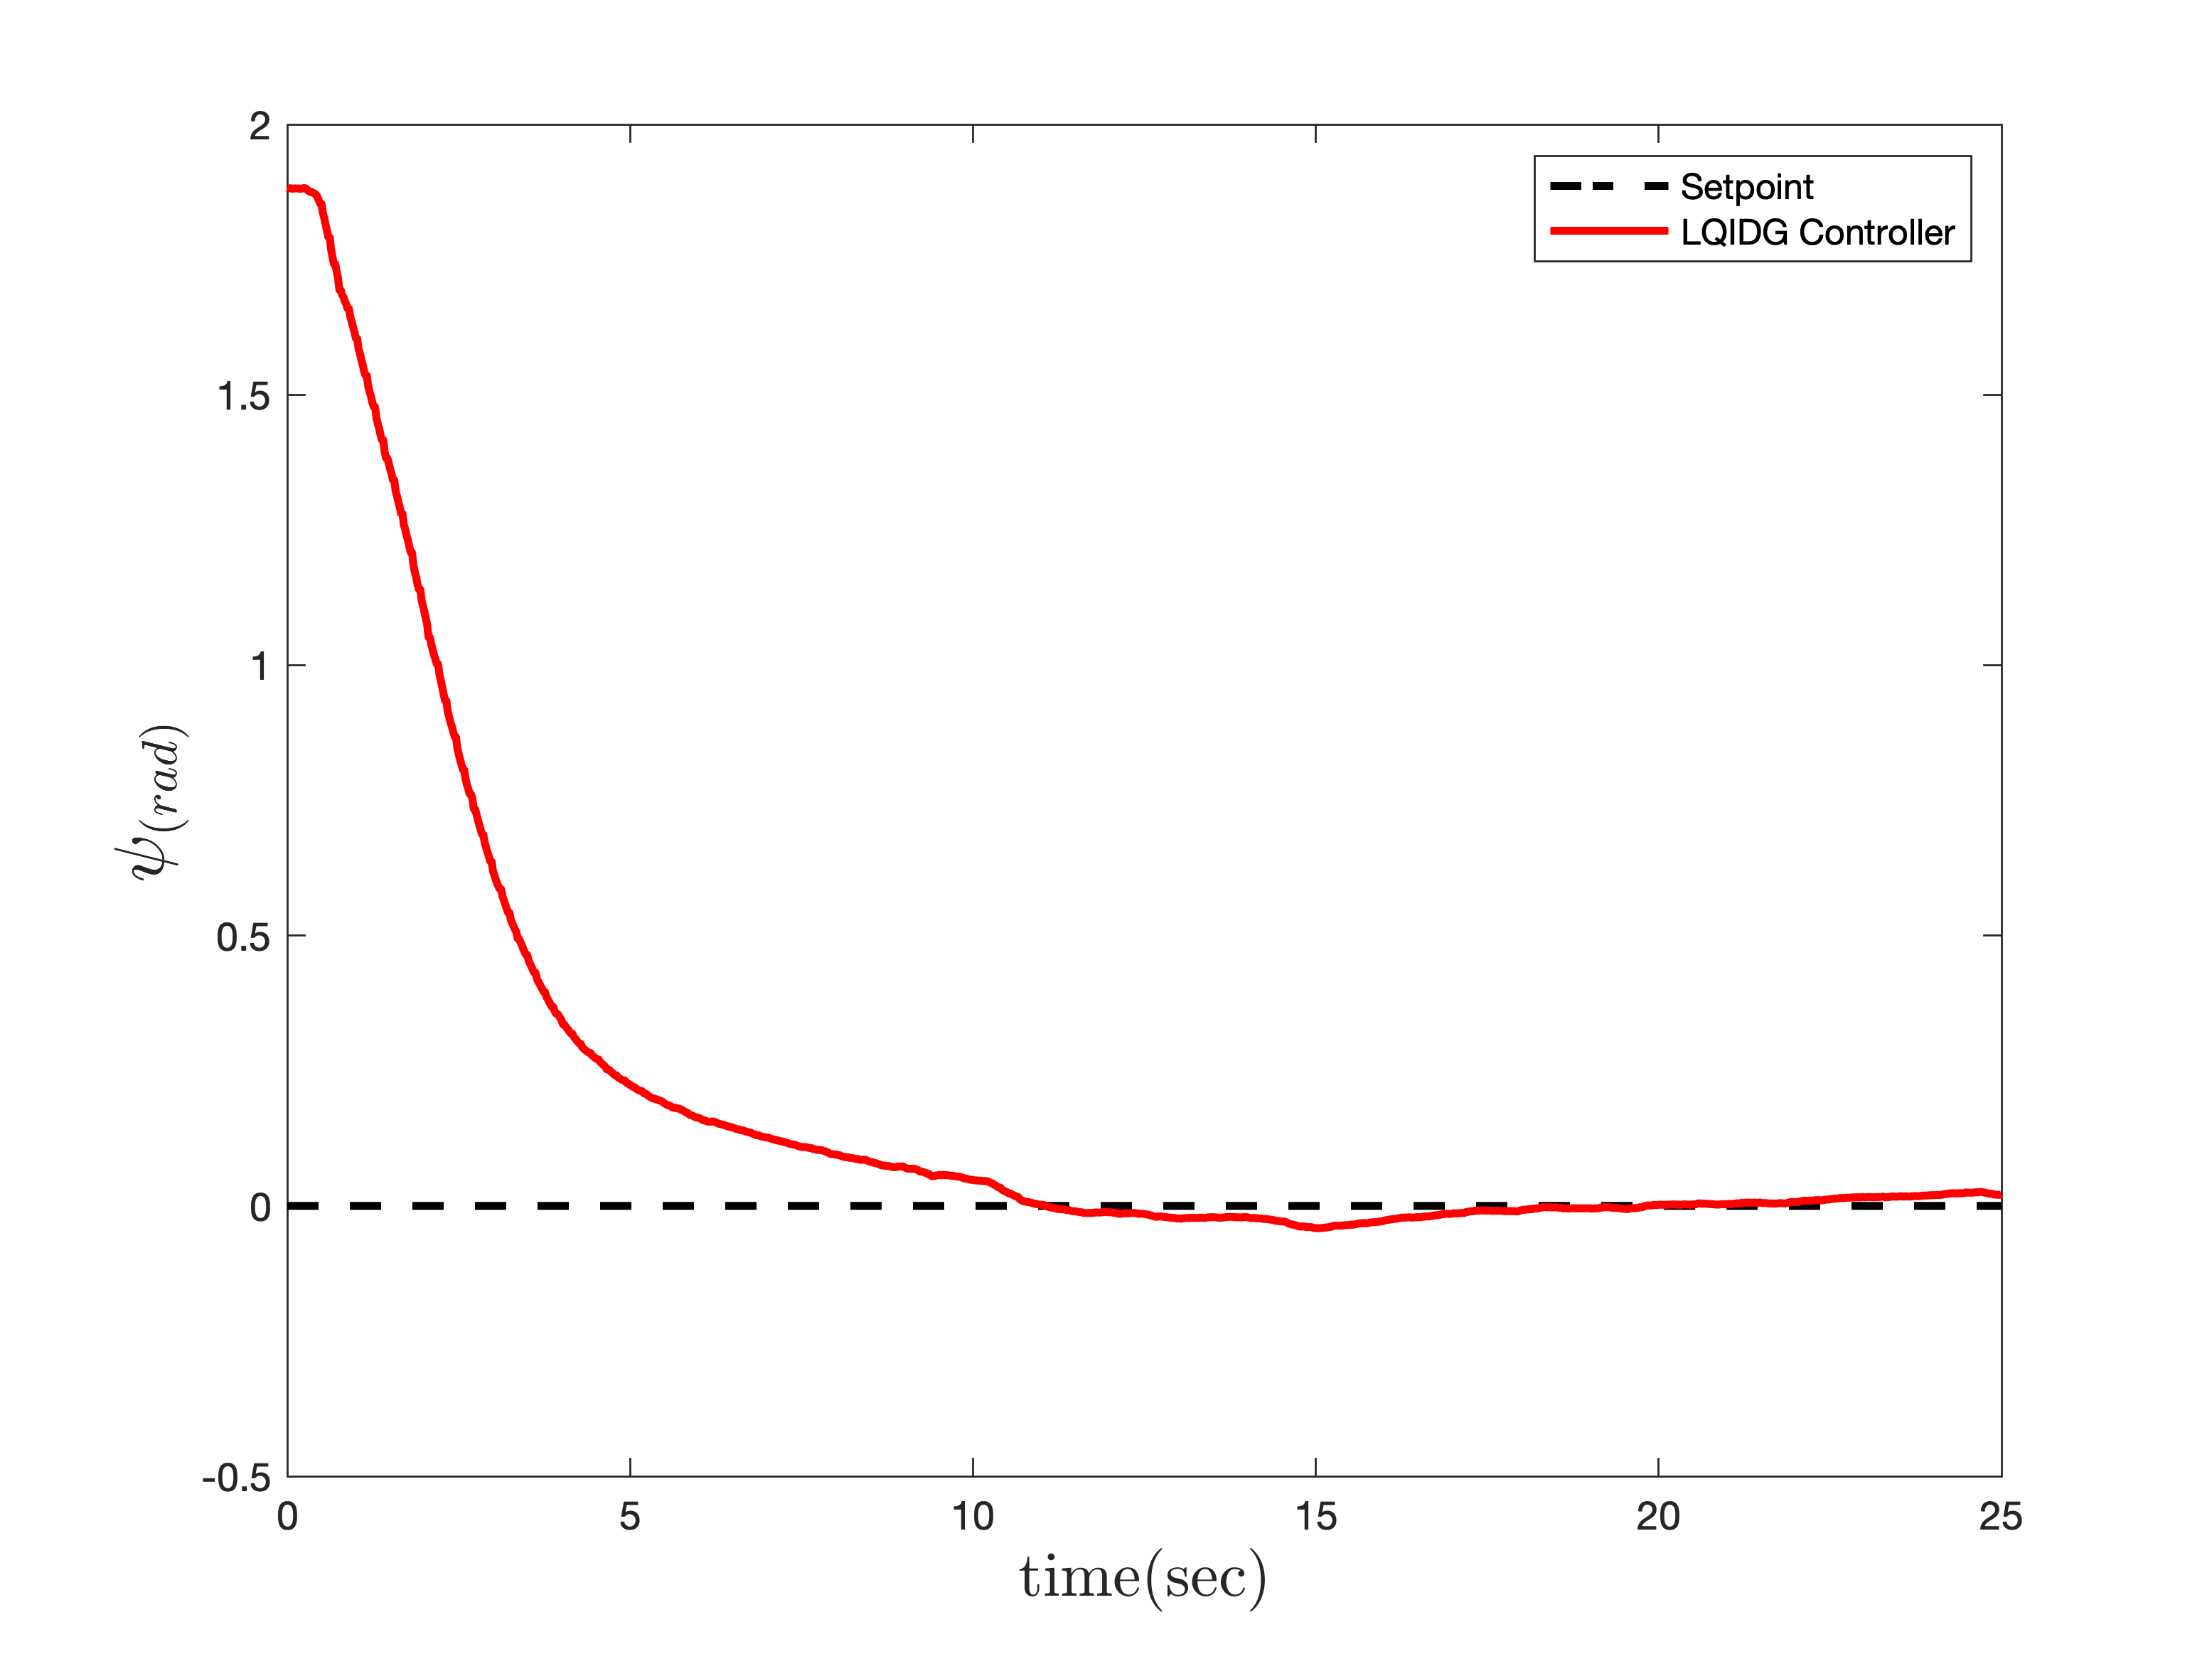
\includegraphics[width=.26\linewidth]{../Figures/Calibration/LQIDG/3DOF/lqidg_yaw.png}}
	\hfil
	\subfloat[]{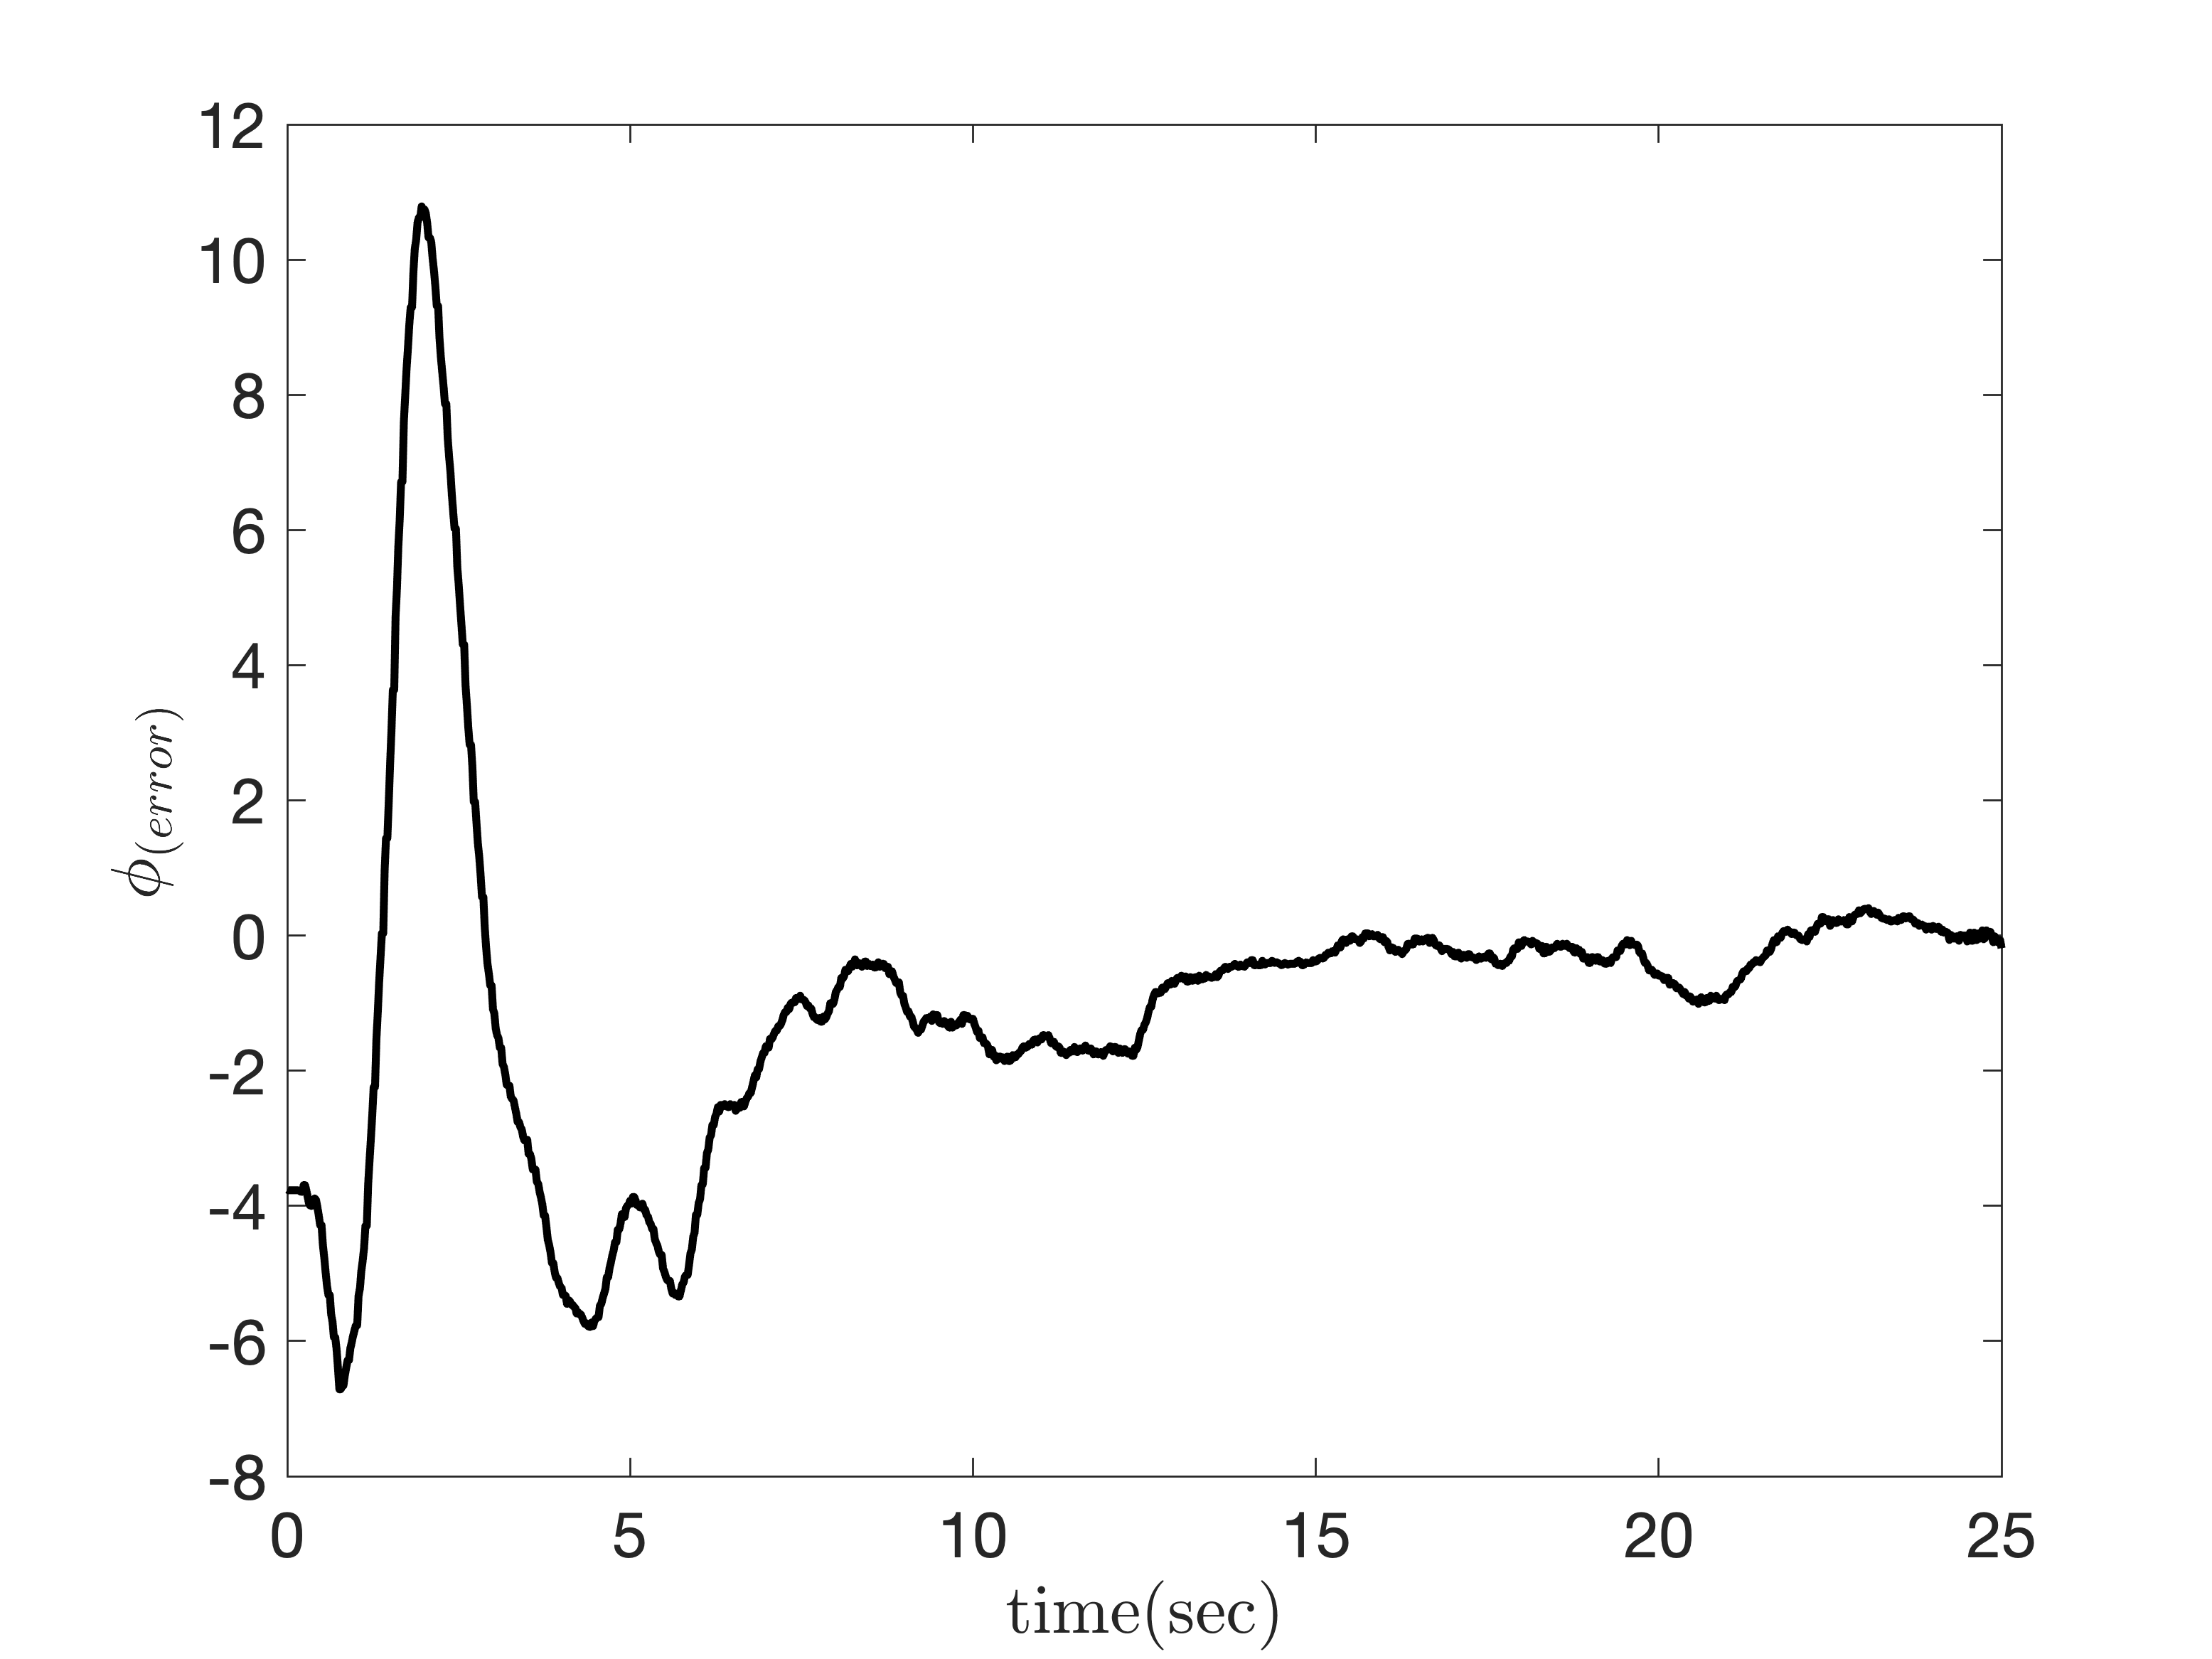
\includegraphics[width=.26\linewidth]{../Figures/Calibration/LQIDG/3DOF/lqidg_roll_e.png}
	}
	\subfloat[]{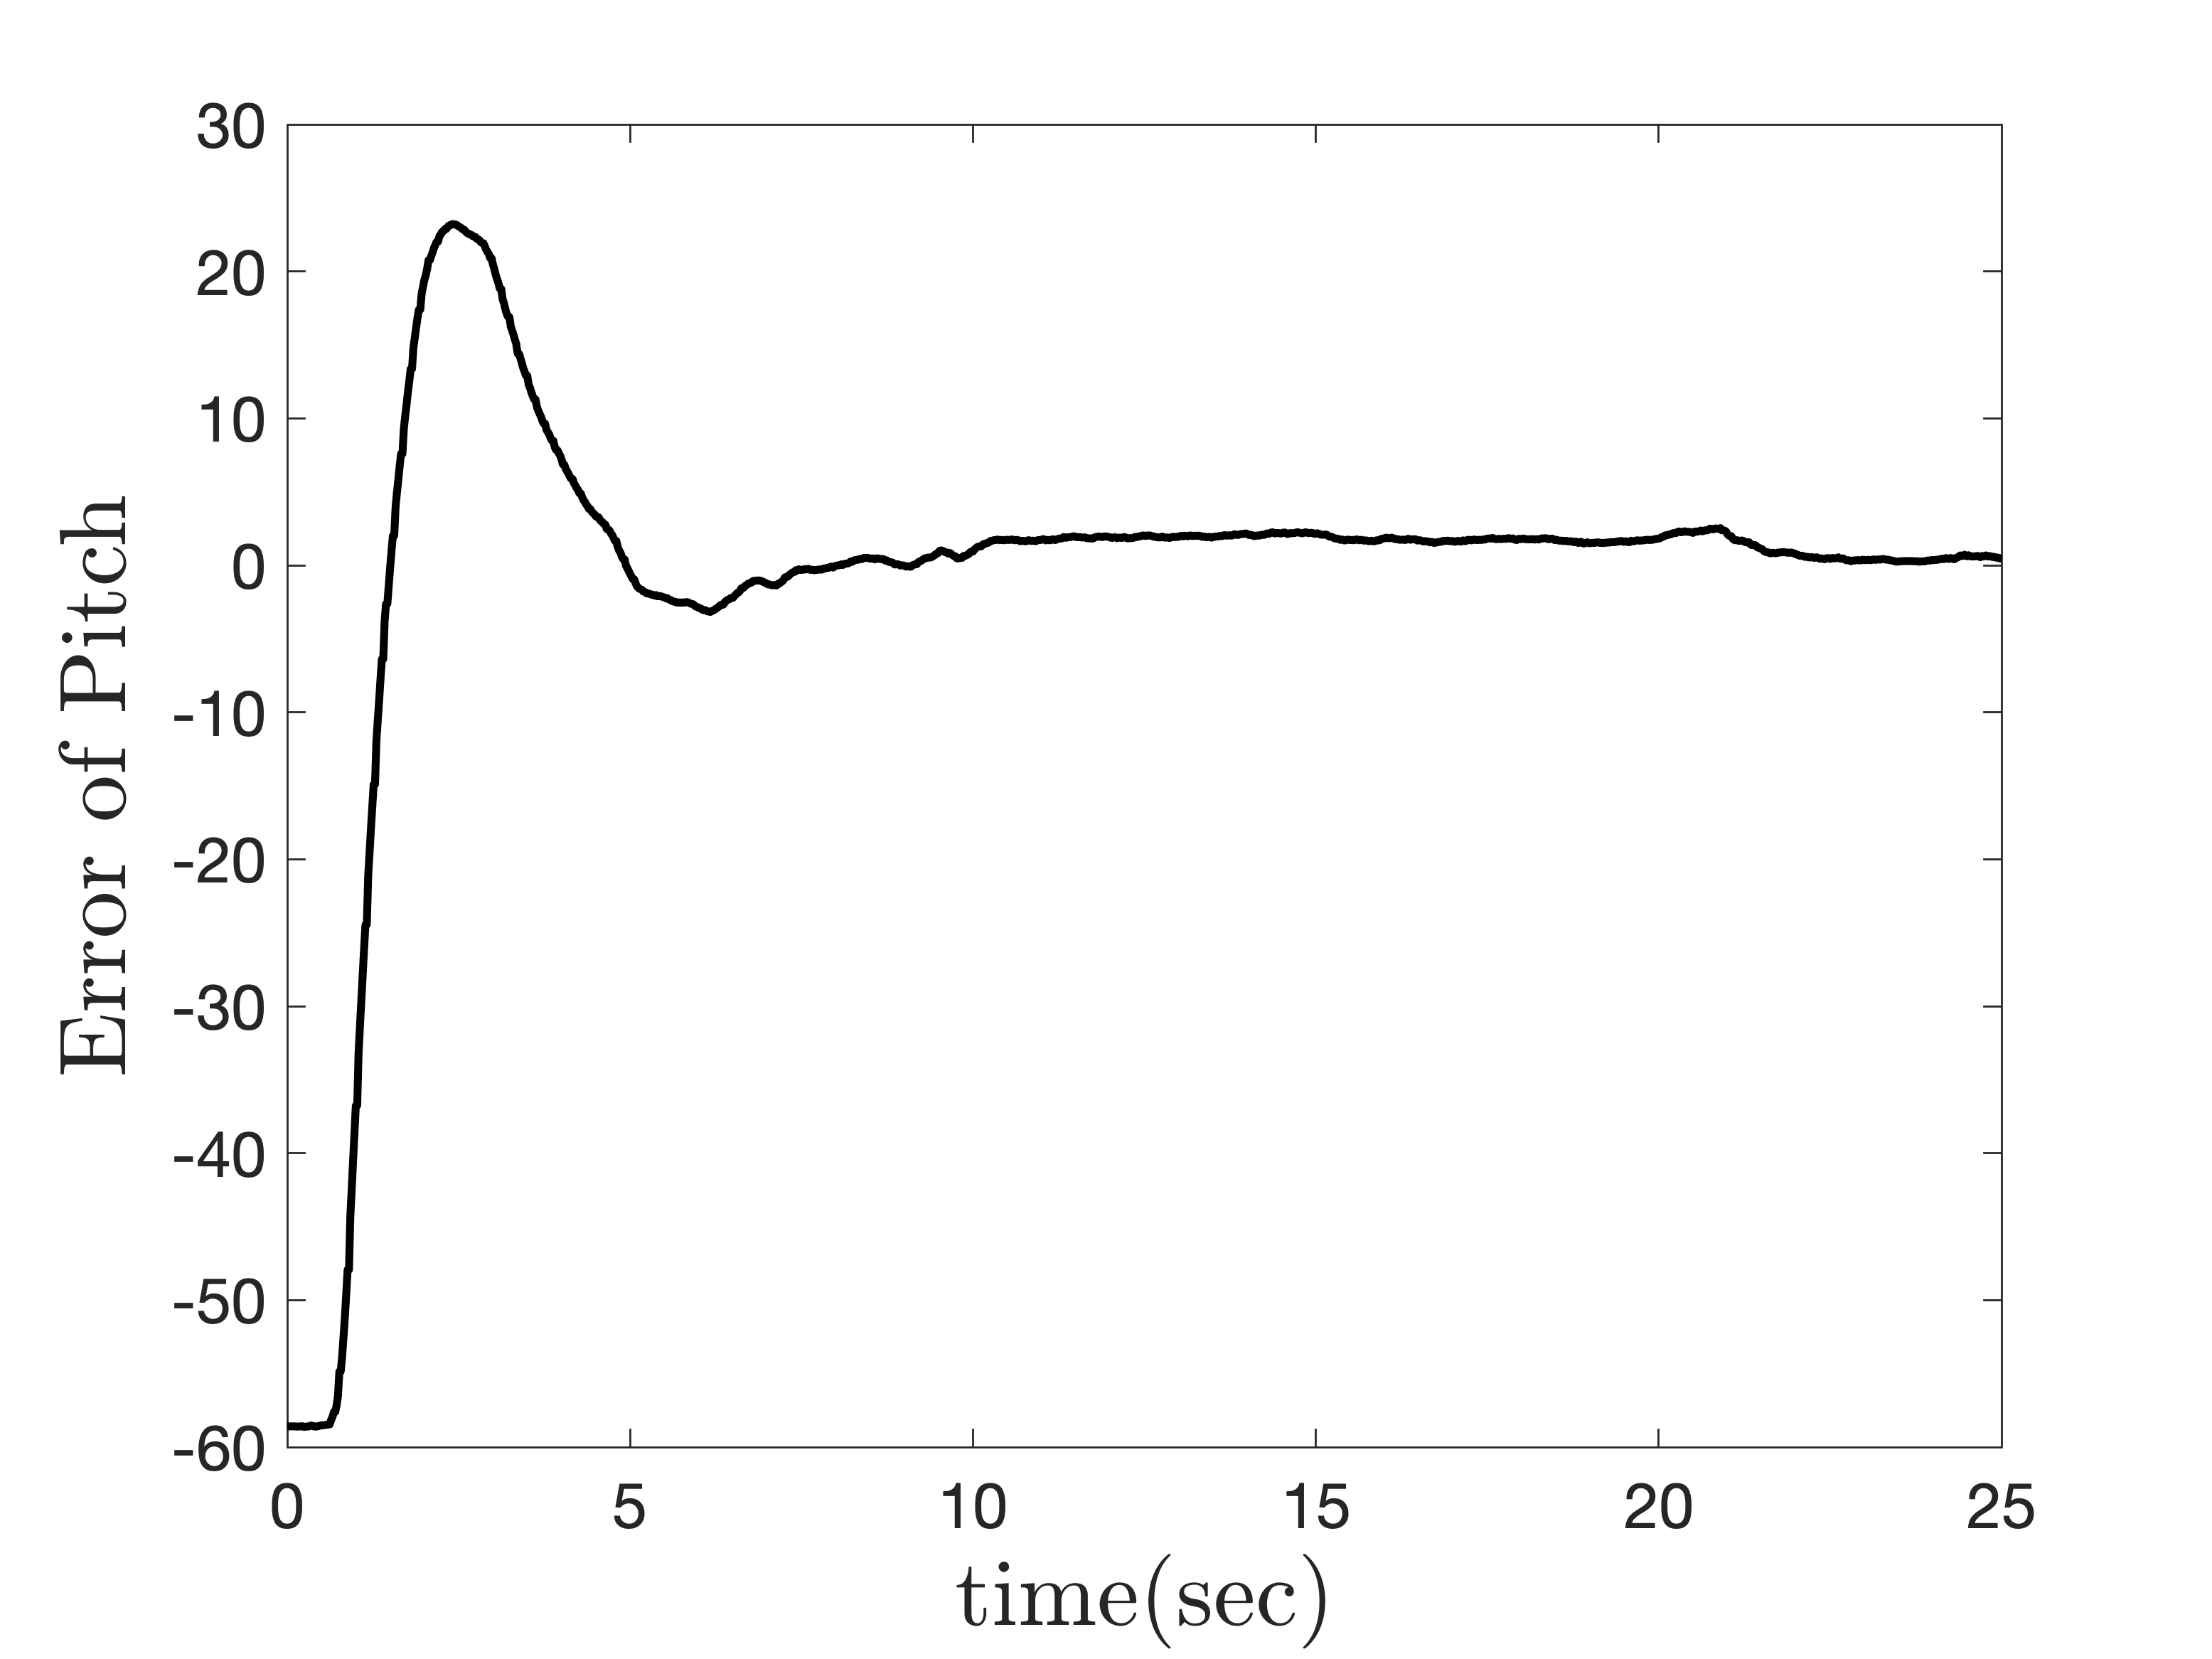
\includegraphics[width=.26\linewidth]{../Figures/Calibration/LQIDG/3DOF/lqidg_pitch_e.png}
	}
	\subfloat[]{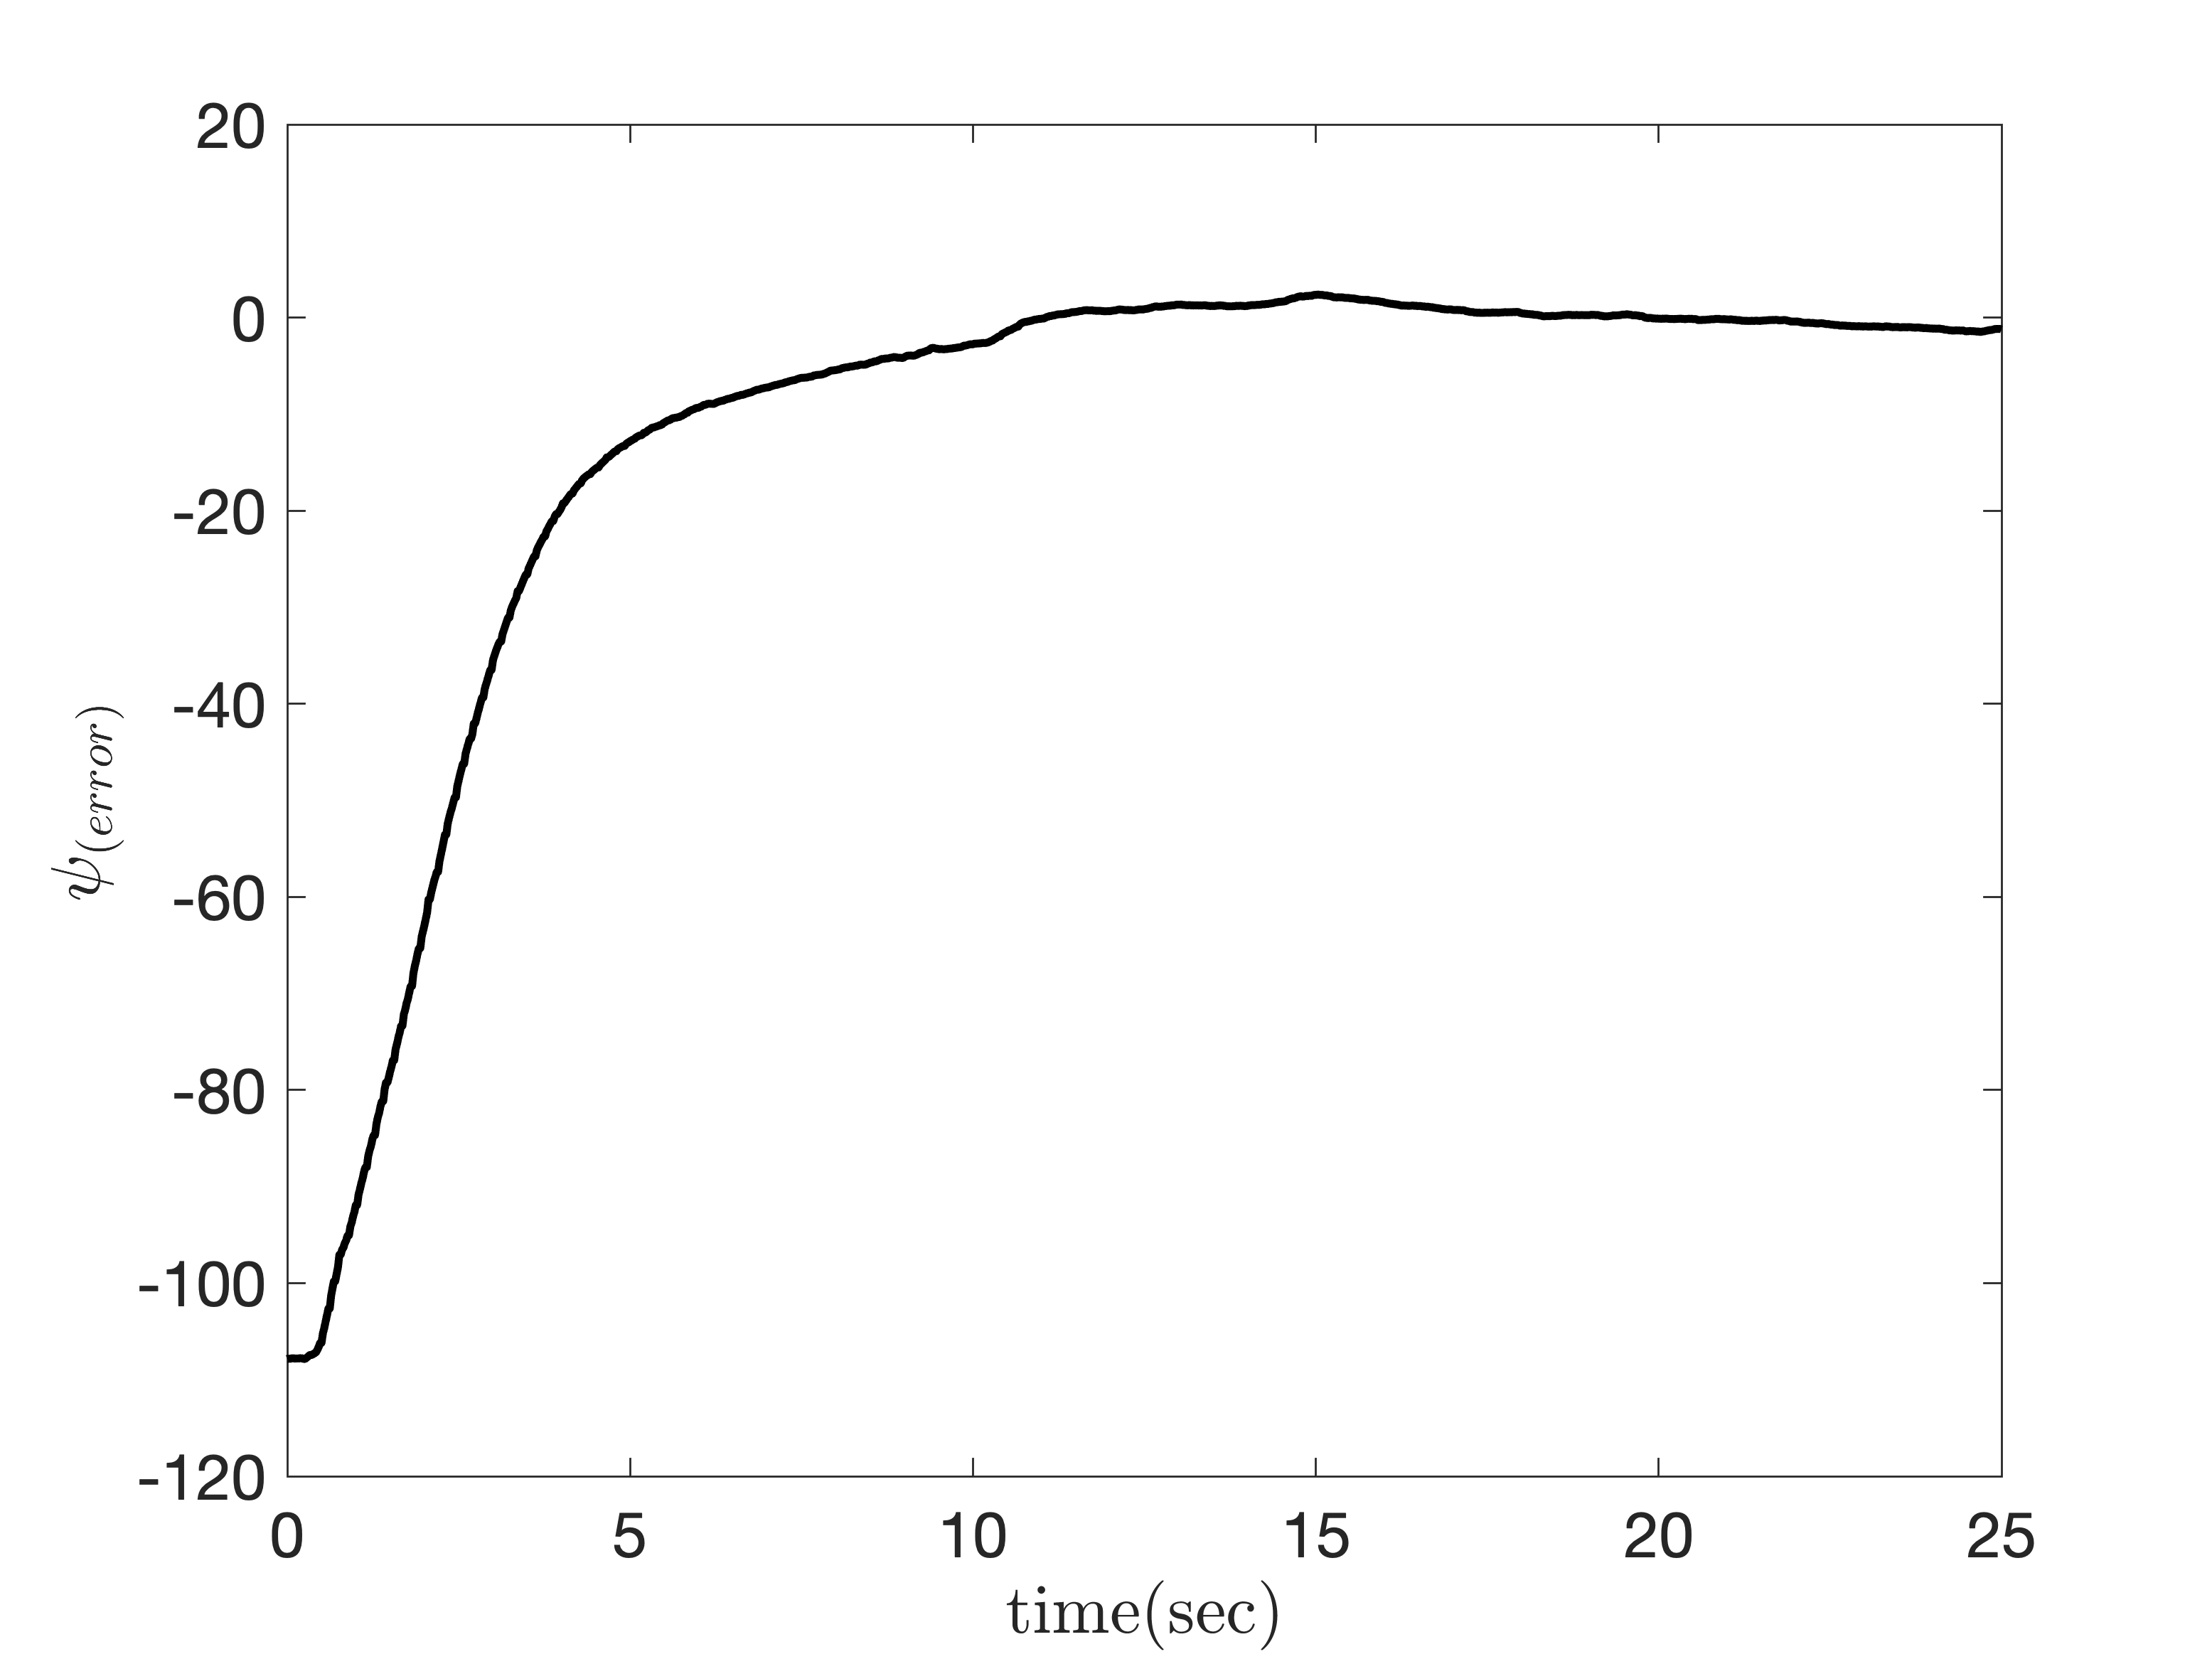
\includegraphics[width=.26\linewidth]{../Figures/Calibration/LQIDG/3DOF/lqidg_yaw_e.png}}
	\caption{Performance of the LQIR-DG controller (a) Desired and actual roll angle (b) Desired and actual pitch angle (c) Desired and actual yaw angle.}
	\label{fig:result}
\end{figure*}

\begin{figure*}[!h]
	\centering
	\subfloat[]{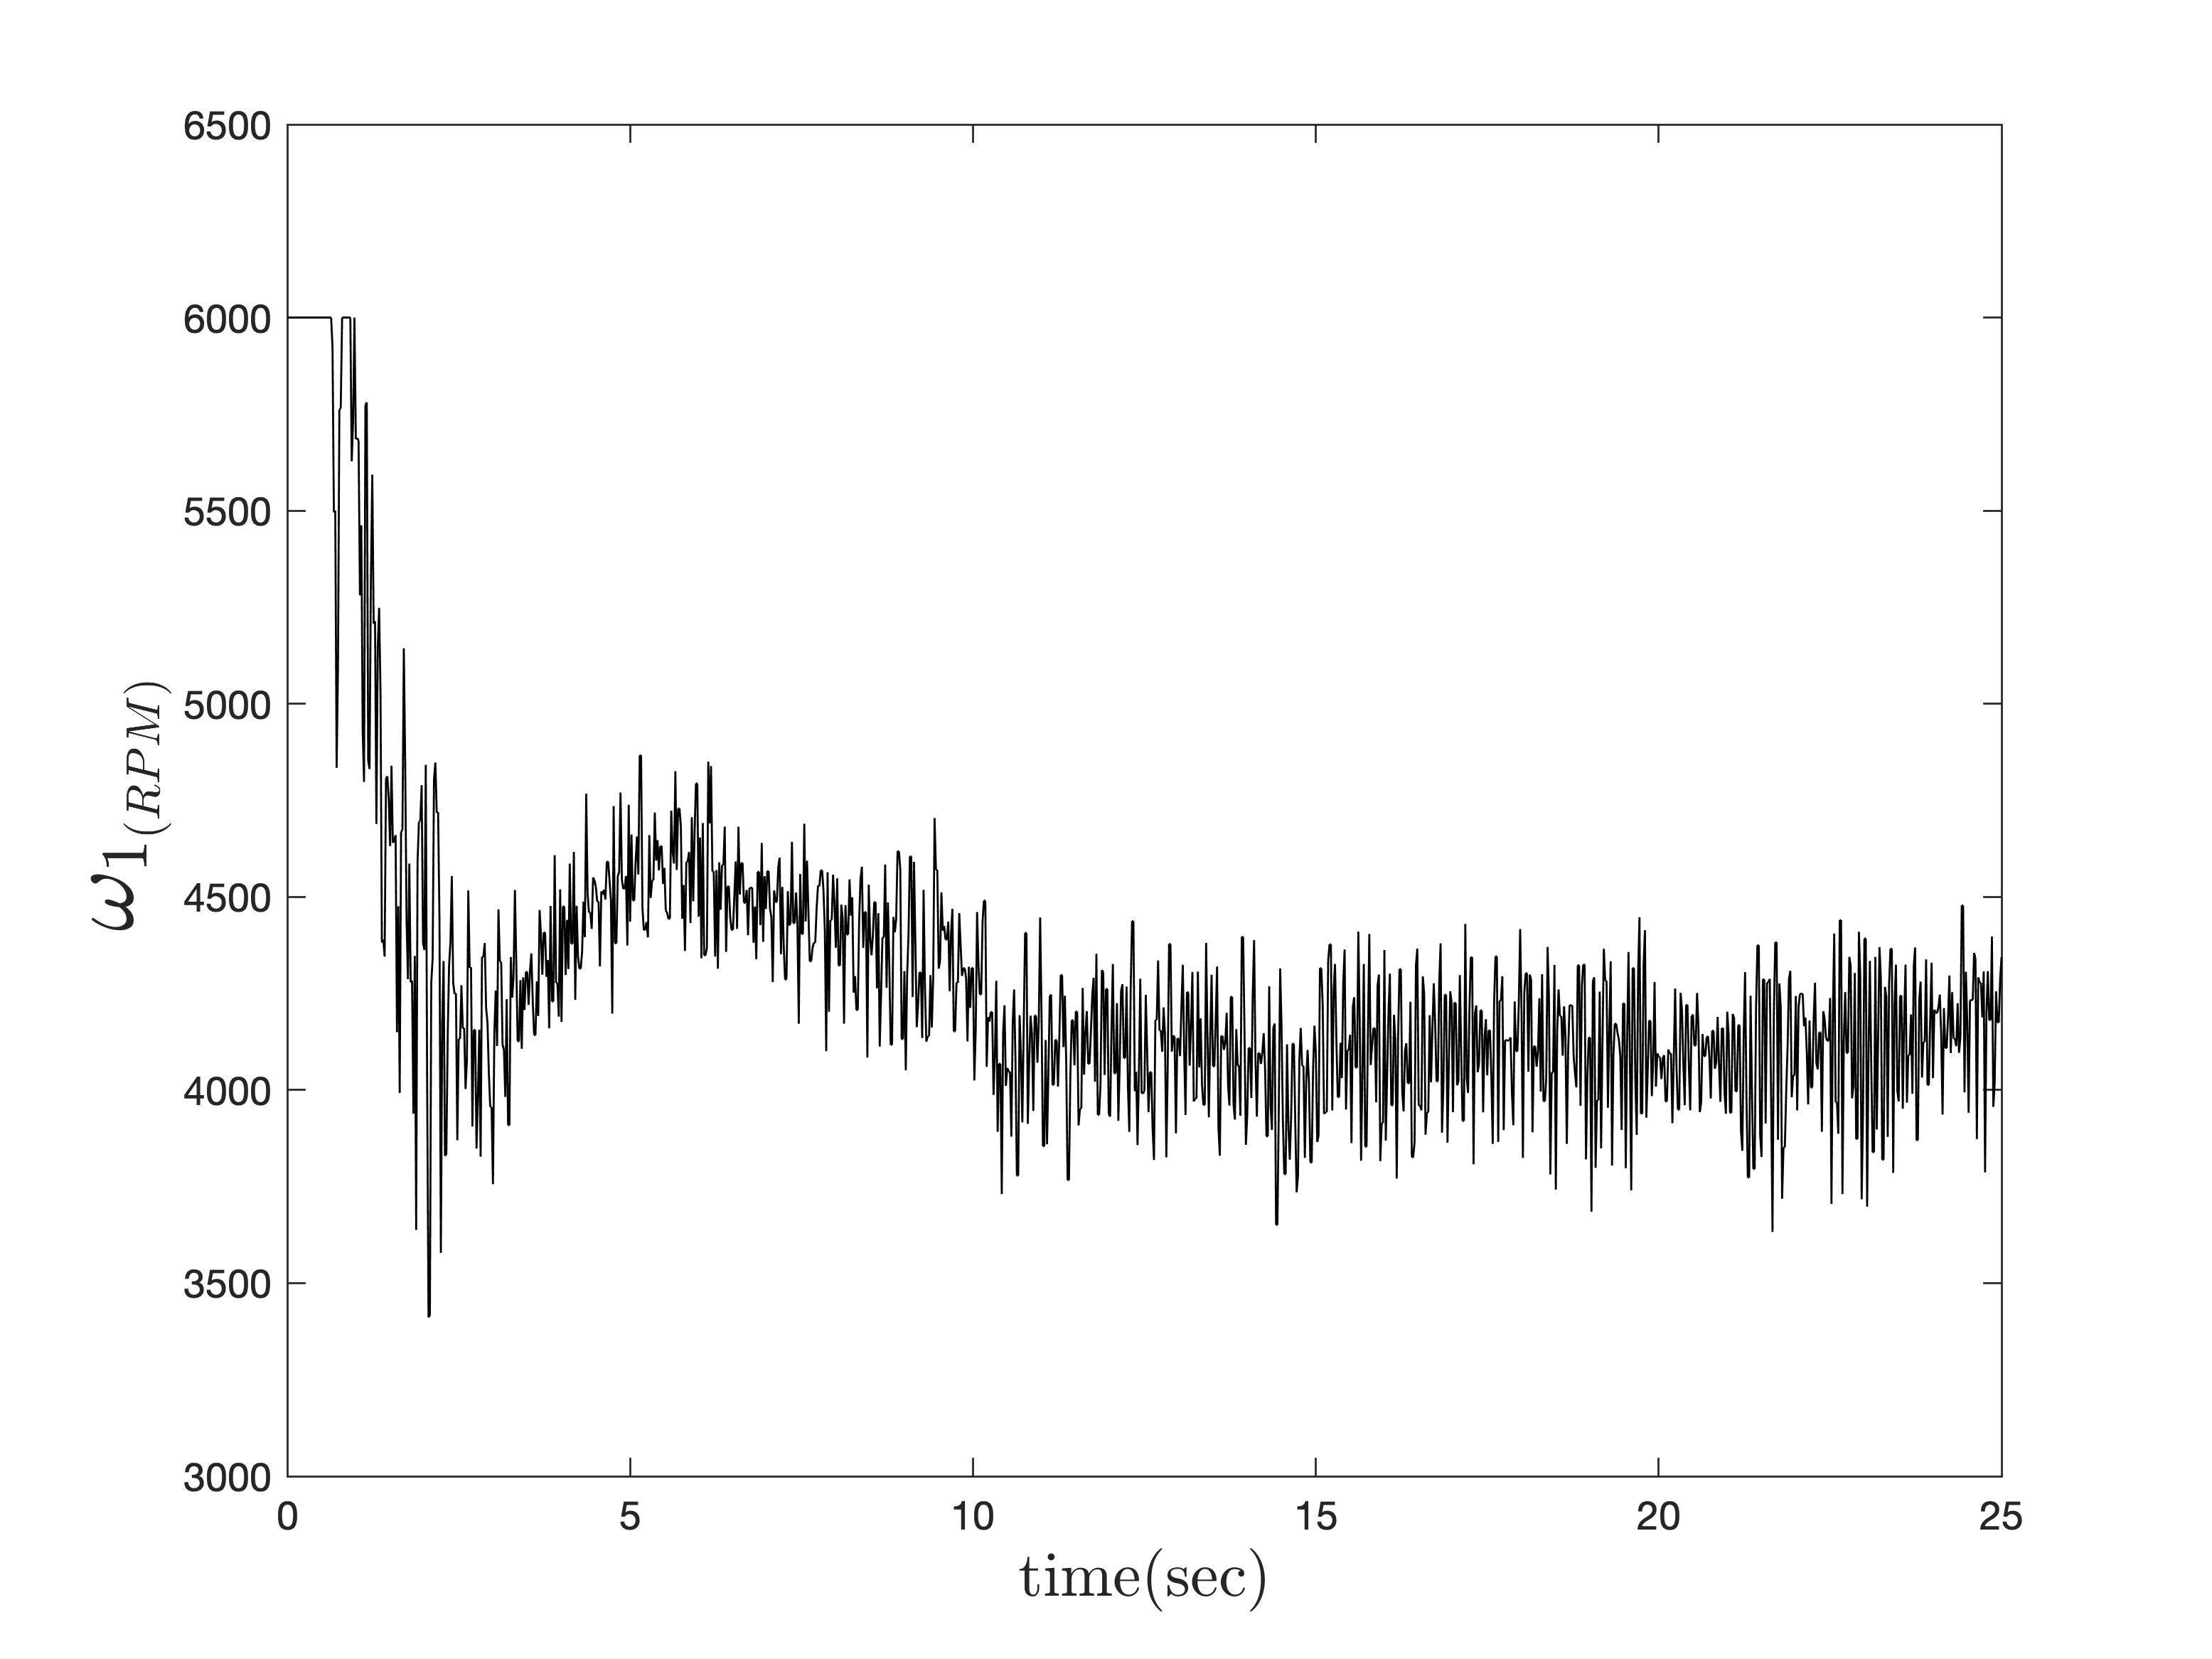
\includegraphics[width=.26\linewidth]{../Figures/Calibration/LQIDG/3DOF/lqidg_Omega_1.png}
	}
	\subfloat[]{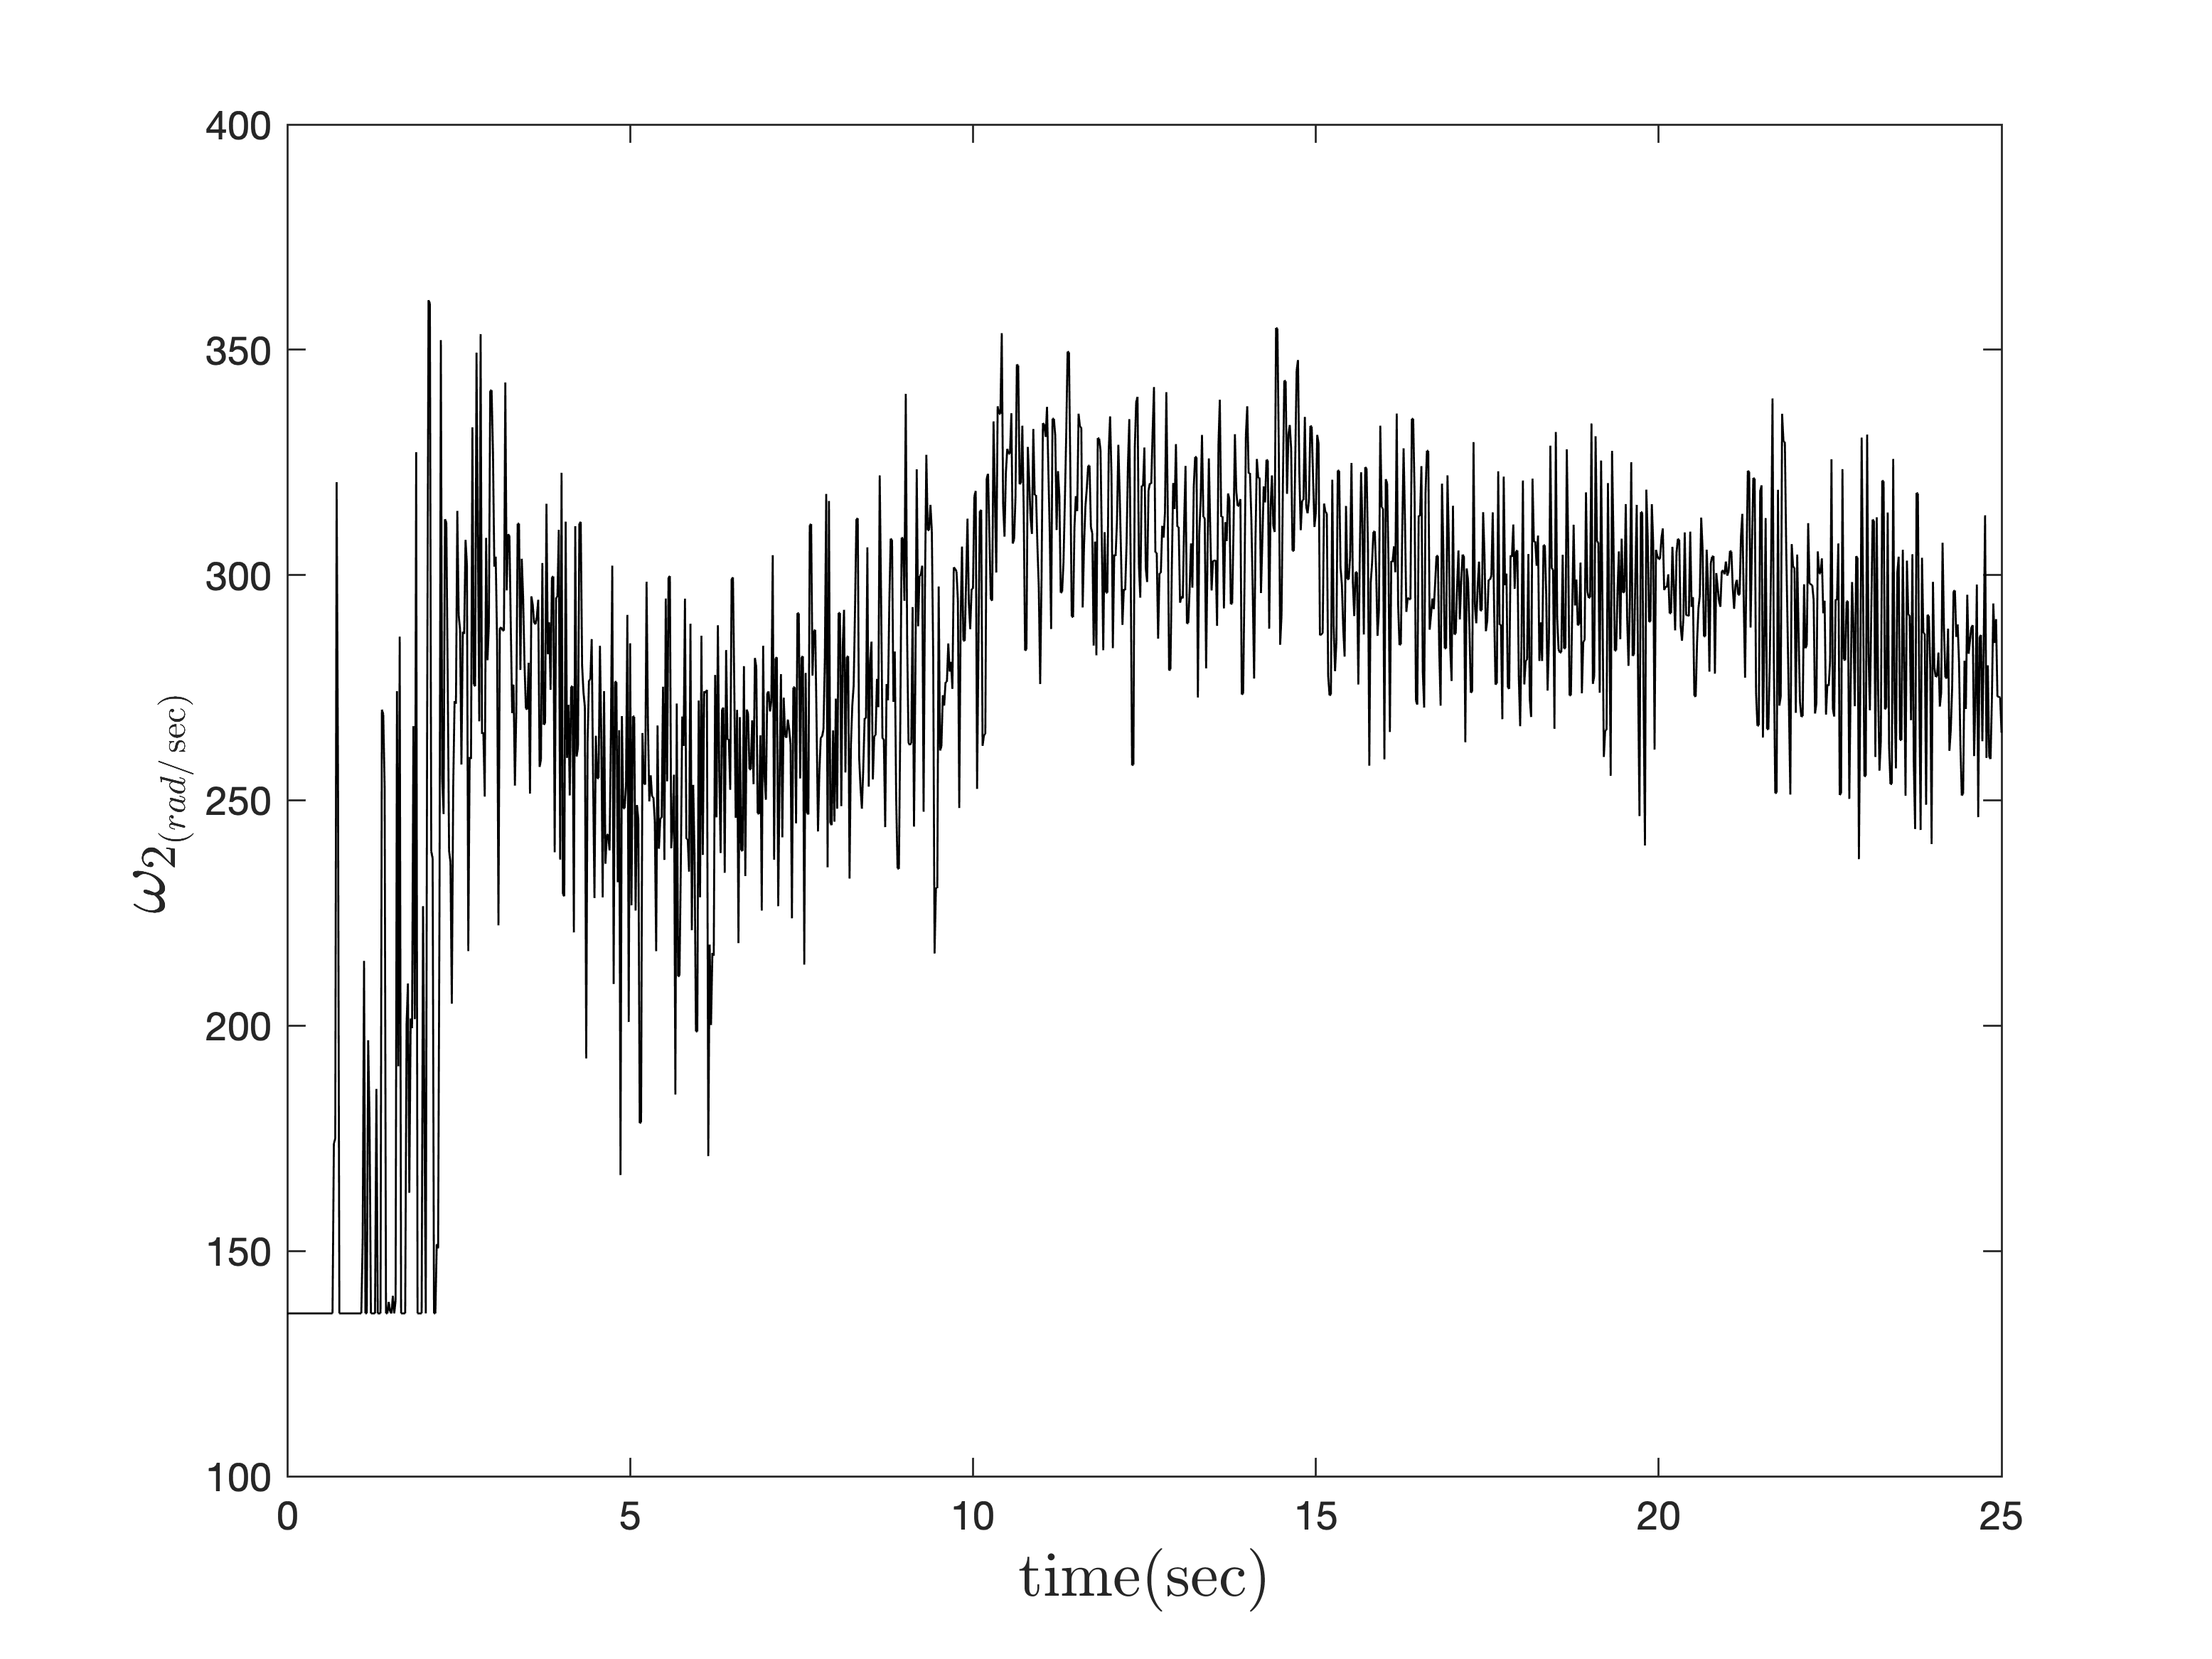
\includegraphics[width=.26\linewidth]{../Figures/Calibration/LQIDG/3DOF/lqidg_Omega_2.png}
	}
	\hfil
	\subfloat[]{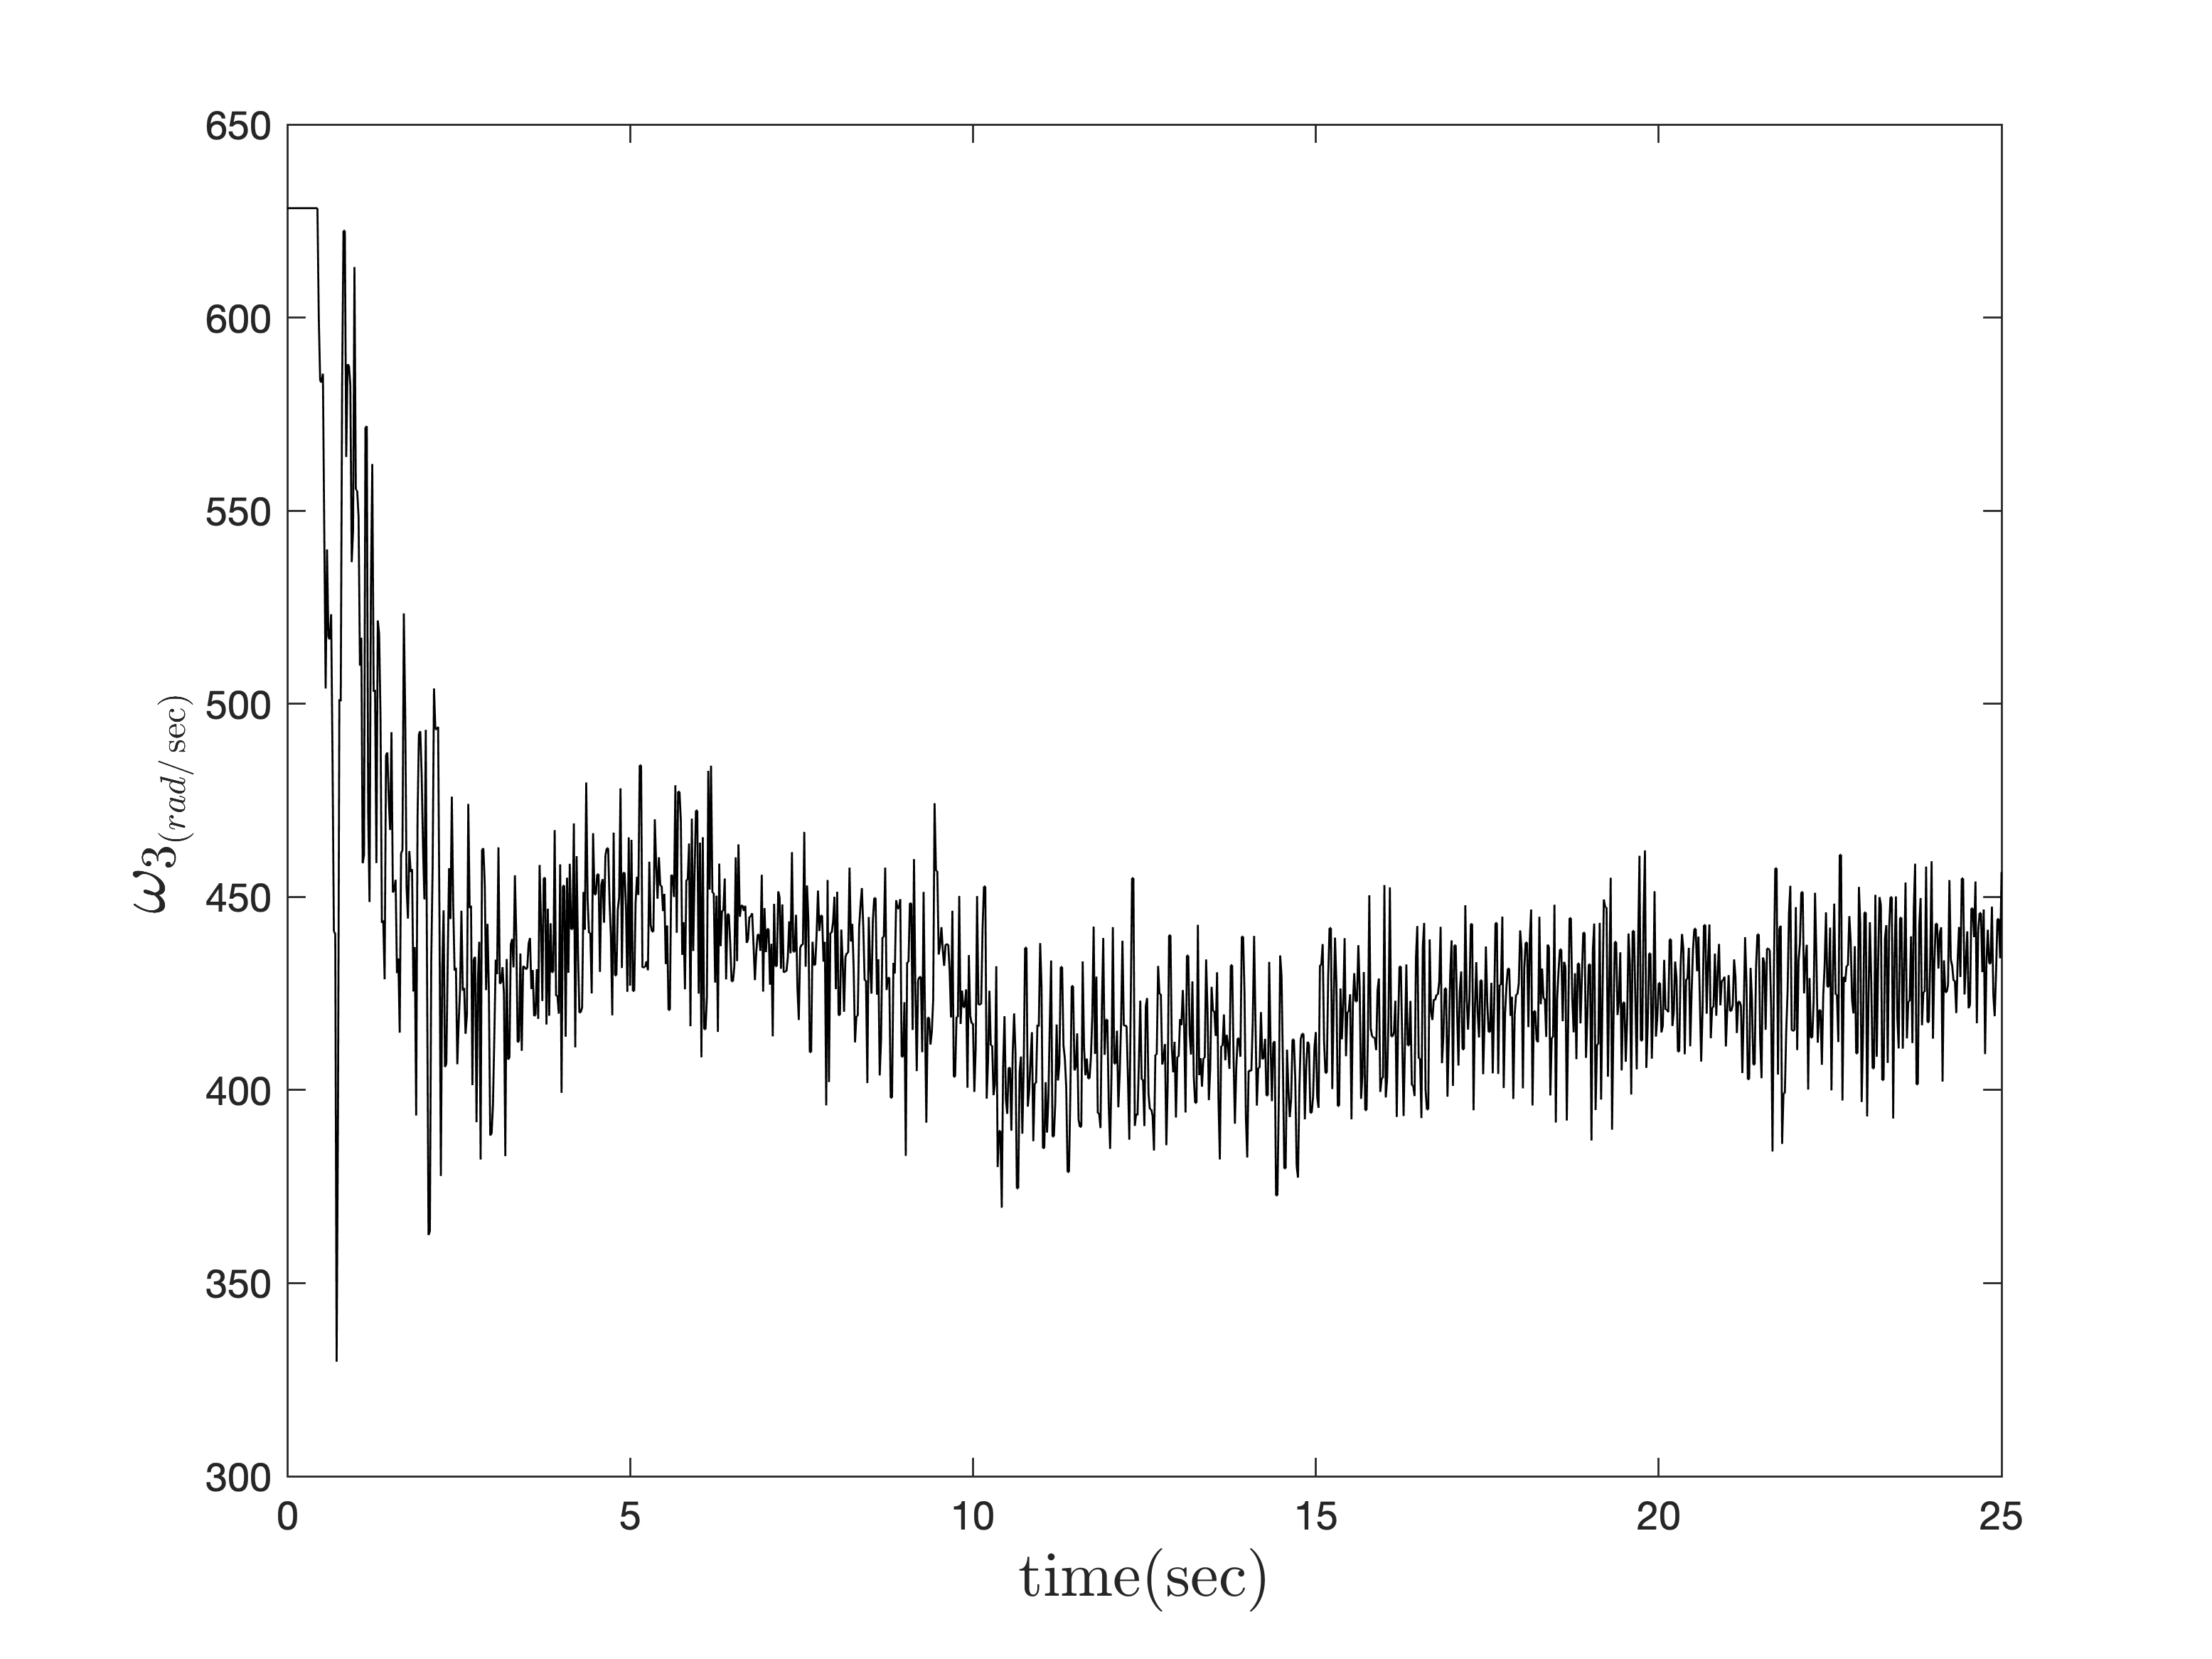
\includegraphics[width=.26\linewidth]{../Figures/Calibration/LQIDG/3DOF/lqidg_Omega_3.png}
	}
	\subfloat[]{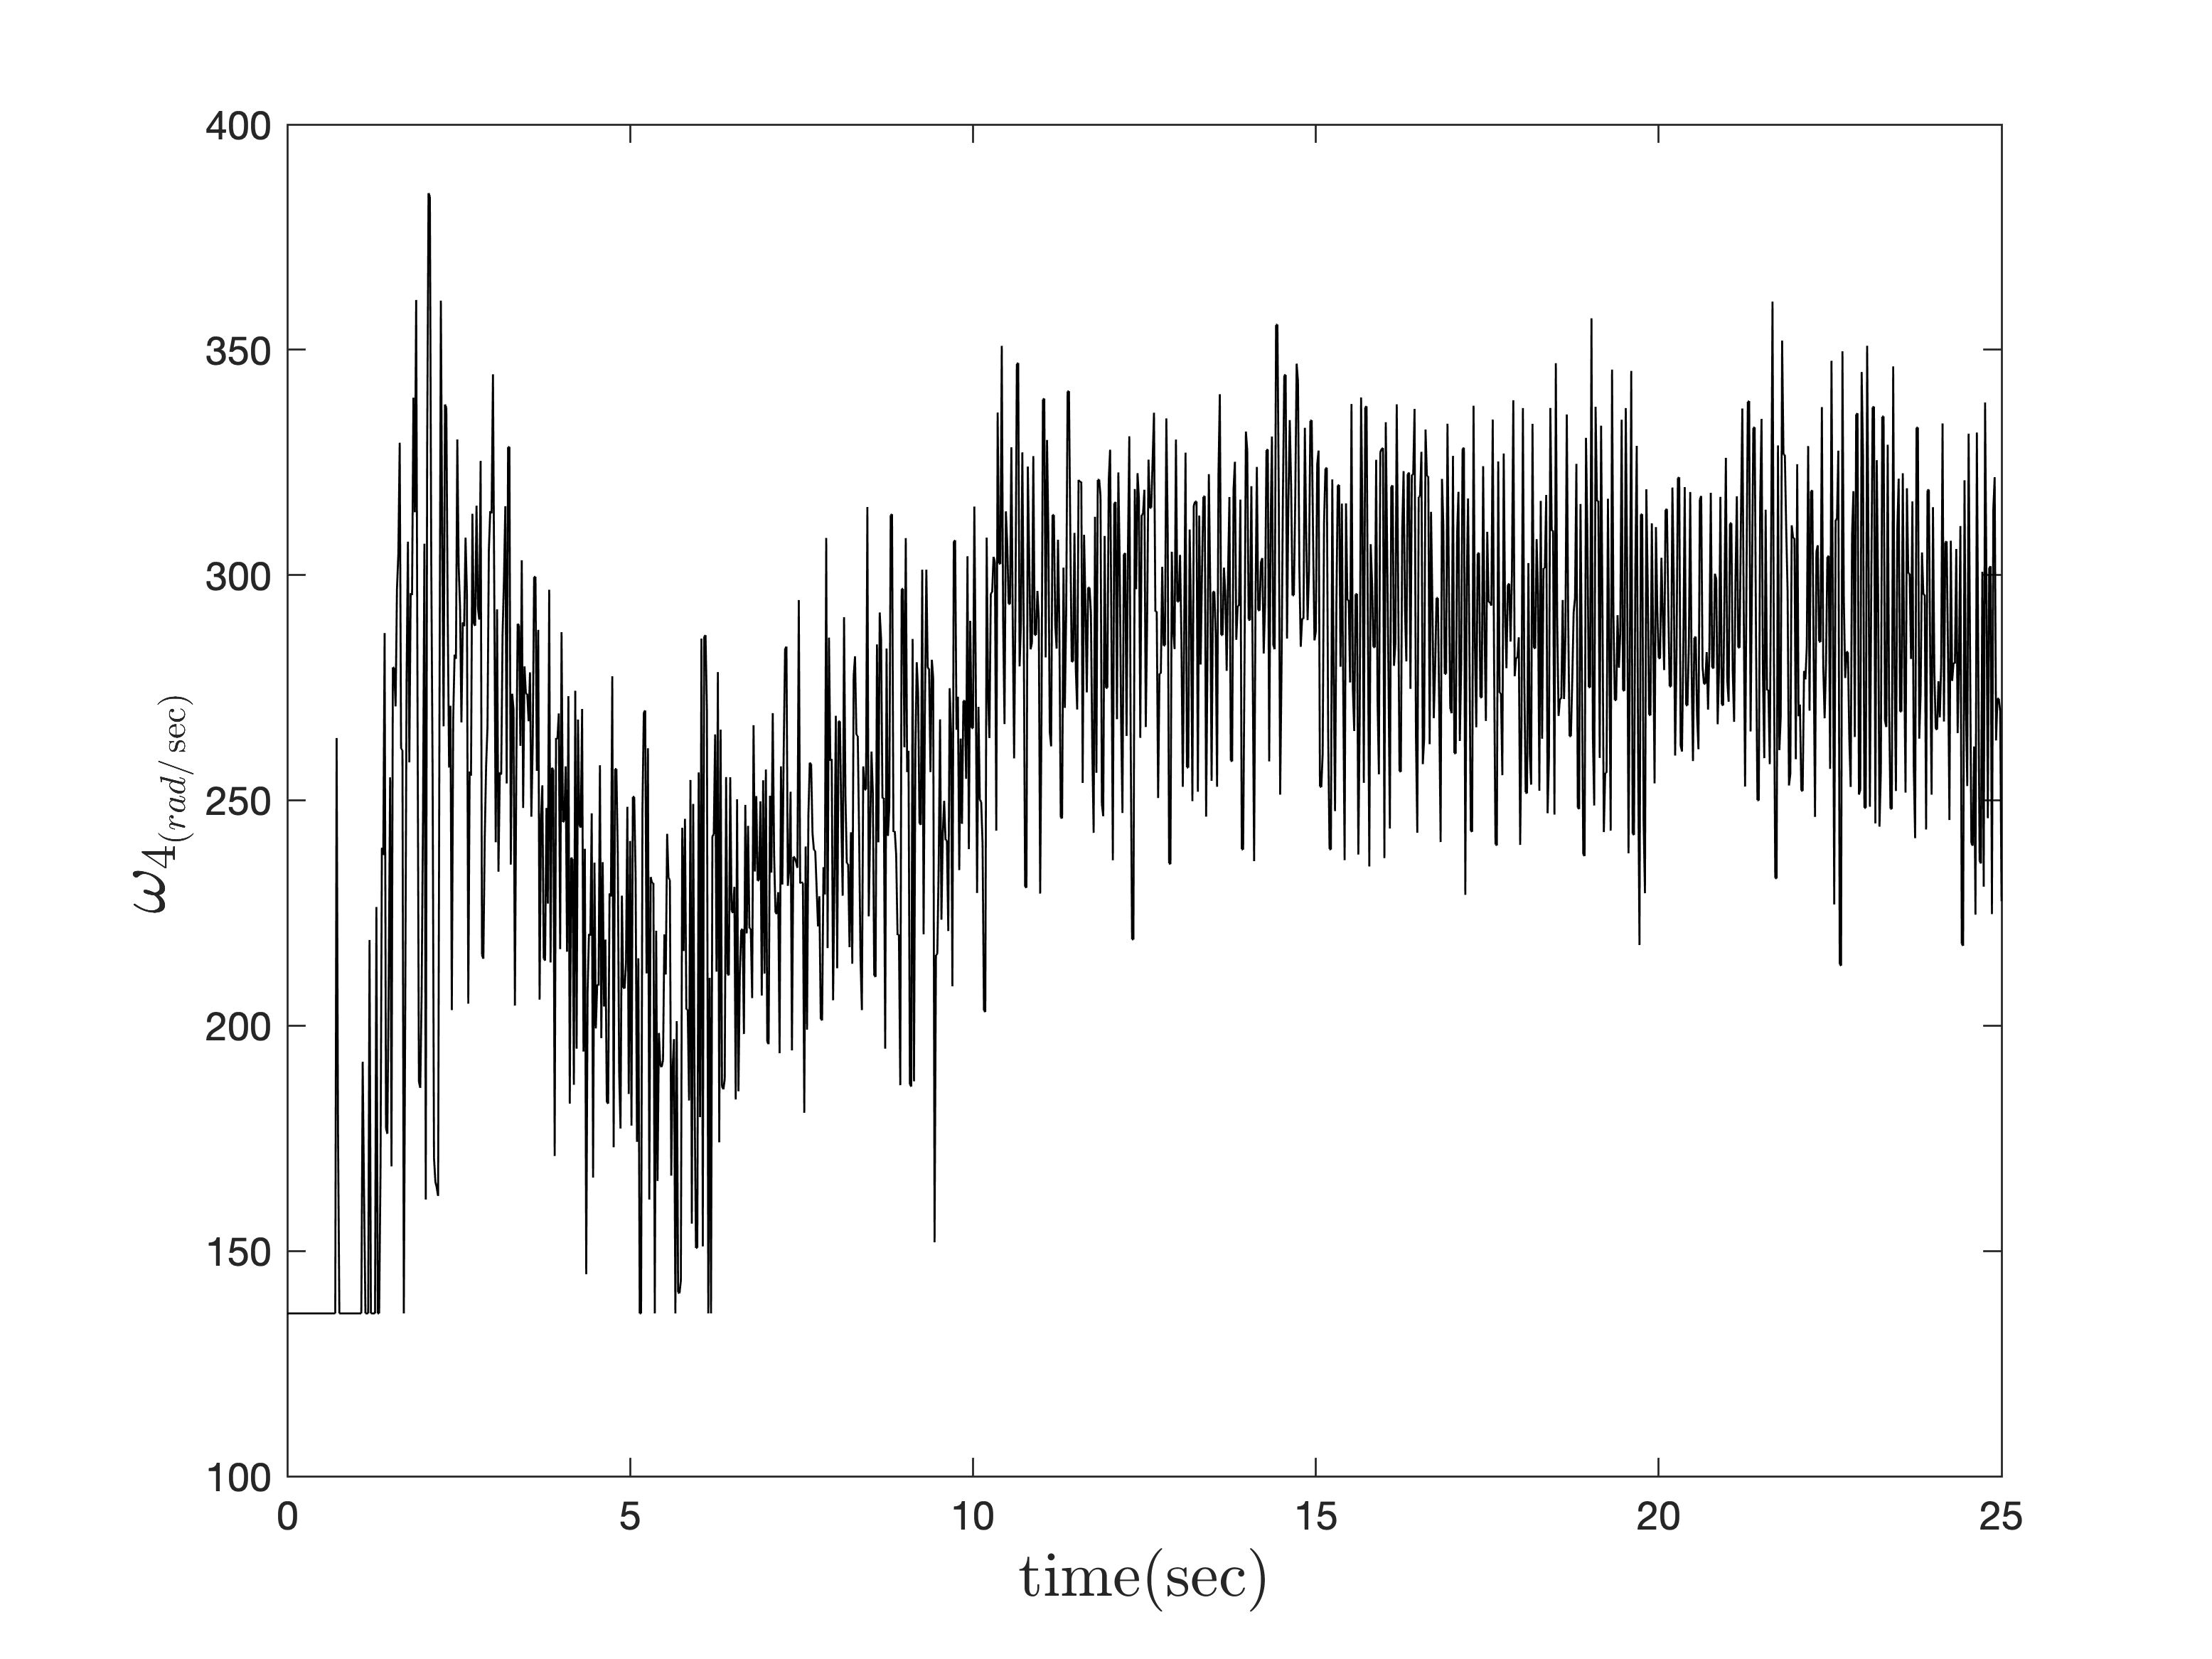
\includegraphics[width=.26\linewidth]{../Figures/Calibration/LQIDG/3DOF/lqidg_Omega_4.png}
	}
	\caption{implementation result omega}
	\label{fig:omega}
\end{figure*}

% \begin{table}[!h]
% 	\renewcommand{\arraystretch}{1.3}
% 	\caption{LQIR-DG Control Parameter}
% 	\begin{center}
% 	\begin{tabular}{c c c c c}
% 	\hline
% 	\textbf{Control Loop} & \textbf{\textit{$q_1$}}& \textbf{\textit{$q_2$}} 
% 	& \textbf{\textit{$q_3$}} & \textbf{\textit{$q_4$}} \\
% 	\hline
% 	Roll & 
% 	$631.85$ & $214.28$ & $7.91$ &
% 	$0.01$ \\
% 	Pitch & 
% 	$0.01$ & $873.93$ & $9853.09$ &
% 	$0.12$ \\
% 	Yaw & 
% 	$3\times10^{-6}$ & $1.7\times10^{-5}$ & $1.81\times10^{-4}$ &
% 	$4.5\times10^{-5}$ \\
% 	\hline
% 	\end{tabular}
% 	\label{tab2}
% 	\end{center}
% \end{table}


\subsection{Comparison with Well-known Control Strategies}



Here, the LQIR-DG controller performance is compared with famous control strategies such as the LQR. \figurename{\ref{fig:compare}} compares the quadrotor's desired and actual pitch angle in the presence of these controllers. These results indicate that the LQIR-DG controller can provide high tracking performance, such as good transient response and high rapid convergence relative to other controllers for pitch angle control of the experimental setup of the quadrotor.


\begin{figure}[!h]
	\centering
	{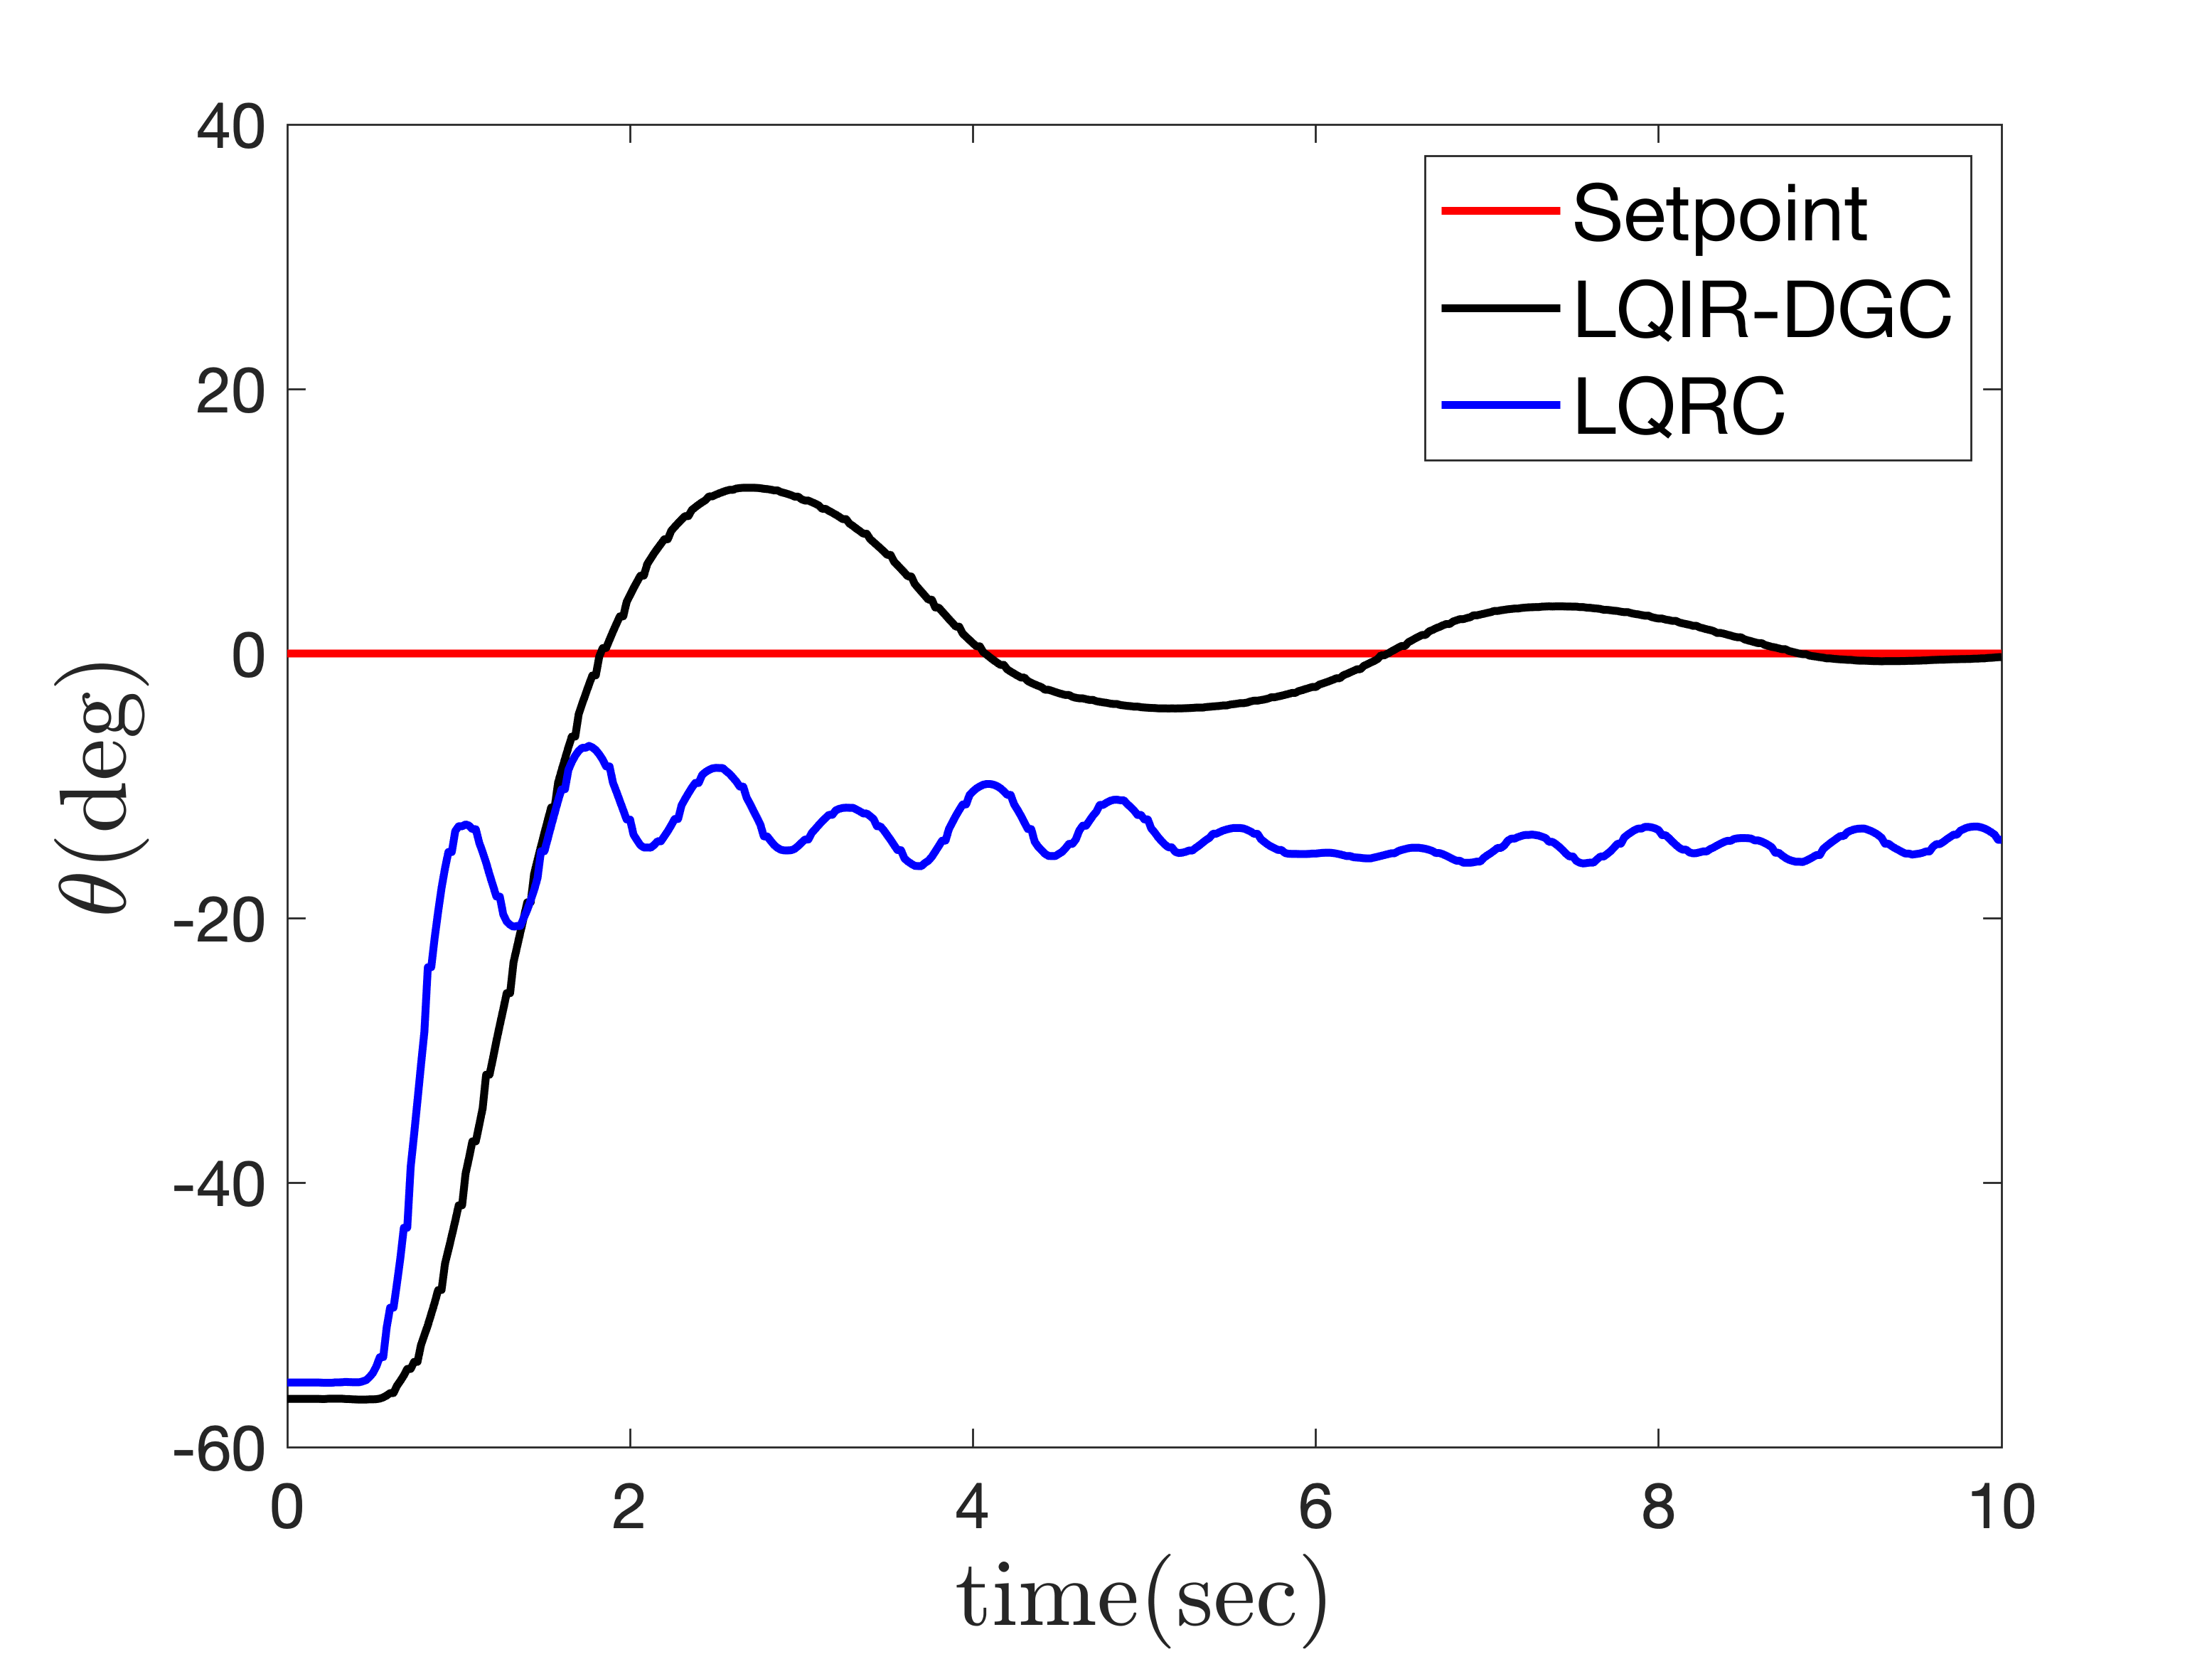
\includegraphics[width=\linewidth]{../Figures/Calibration/LQIDGvsLQR/Pitch/lqidgvslqr_pitch.png}
	}
	\caption{Performance of the LQIR-DG controller vs LQR}
	\label{fig:compare}
\end{figure}


\section{Conclusion}\label{sec:conclusion}
In this study, a linear quadratic with integral action based on the differential game theory, called LQIR-DG, was implemented for level attitude control in an experimental setup of a quadrotor. To implement the proposed controller structure, first, an accurate dynamic model of the quadrotor was linearized in the state-space form, and then the model parameters were estimated. Next, two players were considered for each of the quadrotor's roll, pitch, and yaw channels. The first player found the best control command for each channel of the setup of a quadrotor based on the minimization of a quadratic criterion; when the second player produced the disturbances. Finally, the performance of the proposed controller was evaluated in level flight and compared to the LQR controller. The implementation results verify the successful performance of the LQIR-DG method in the level of attitude control of the experimental setup of the quadrotor.






% \begin{figure*}[!t]
% 	\centering
% 	\subfloat[Case I]{\includegraphics[width=2.5in]{subf igcase1}
% 	\label{fig_first_case}}
% 	\hfil
% 	\subfloat[Case II]{\includegraphics[width=2.5in]{sub figcase2}
% 	\label{fig_second_case}}
% 	\caption{Simulation results for the network.} \label{fig_sim}
% \end{figure*}




% Before you begin to format your paper, first write and save the content as a 
% separate text file. Complete all content and organizational editing before 
% formatting. Please note sections \eqref{AA}--\eqref{SCM} below for more information on 
% proofreading, spelling and grammar.
% Keep your text and graphic files separate until after the text has been 
% formatted and styled. Do not number text heads---{\LaTeX} will do that 
% for you.
% \subsection{Abbreviations and Acronyms}\label{AA}
% Define abbreviations and acronyms the first time they are used in the text, 
% even after they have been defined in the abstract. Abbreviations such as 
% IEEE, SI, MKS, CGS, ac, dc, and rms do not have to be defined. Do not use 
% abbreviations in the title or heads unless they are unavoidable.

% \subsection{Units}
% \begin{itemize}
% \item Use either SI (MKS) or CGS as primary units. (SI units are encouraged.) English units may be used as secondary units (in parentheses). An exception would be the use of English units as identifiers in trade, such as ``3.5-inch disk drive''.
% \item Avoid combining SI and CGS units, such as current in amperes and magnetic field in oersteds. This often leads to confusion because equations do not balance dimensionally. If you must use mixed units, clearly state the units for each quantity that you use in an equation.
% \item Do not mix complete spellings and abbreviations of units: ``Wb/m\textsuperscript{2}'' or ``webers per square meter'', not ``webers/m\textsuperscript{2}''. Spell out units when they appear in text: ``. . . a few henries'', not ``. . . a few H''.
% \item Use a zero before decimal points: ``0.25'', not ``.25''. Use ``cm\textsuperscript{3}'', not ``cc''.)
% \end{itemize}

% \subsection{Equations}
% Number equations consecutively. To make your 
% equations more compact, you may use the solidus (~/~), the exp function, or 
% appropriate exponents. Italicize Roman symbols for quantities and variables, 
% but not Greek symbols. Use a long dash rather than a hyphen for a minus 
% sign. Punctuate equations with commas or periods when they are part of a 
% sentence, as in:
% \begin{equation}
% a+b=\gamma\label{eq}
% \end{equation}

% Be sure that the 
% symbols in your equation have been defined before or immediately following 
% the equation. Use ``\eqref{eq}'', not ``Eq.~\eqref{eq}'' or ``equation \eqref{eq}'', except at 
% the beginning of a sentence: ``Equation \eqref{eq} is . . .''

% \subsection{\LaTeX-Specific Advice}

% Please use ``soft'' (e.g., \verb|\eqref{Eq}|) cross references instead
% of ``hard'' references (e.g., \verb|(1)|). That will make it possible
% to combine sections, add equations, or change the order of figures or
% citations without having to go through the file line by line.

% Please don't use the \verb|{eqnarray}| equation environment. Use
% \verb|{align}| or \verb|{IEEEeqnarray}| instead. The \verb|{eqnarray}|
% environment leaves unsightly spaces around relation symbols.

% Please note that the \verb|{subequations}| environment in {\LaTeX}
% will increment the main equation counter even when there are no
% equation numbers displayed. If you forget that, you might write an
% article in which the equation numbers skip from (17) to (20), causing
% the copy editors to wonder if you've discovered a new method of
% counting.

% {\BibTeX} does not work by magic. It doesn't get the bibliographic
% data from thin air but from .bib files. If you use {\BibTeX} to produce a
% bibliography you must send the .bib files. 

% {\LaTeX} can't read your mind. If you assign the same label to a
% subsubsection and a table, you might find that Table I has been cross
% eqreferenced as Table IV-B3. 

% {\LaTeX} does not have precognitive abilities. If you put a
% \verb|\label| command before the command that updates the counter it's
% supposed to be using, the label will pick up the last counter to be
% cross referenced instead. In particular, a \verb|\label| command
% should not go before the caption of a figure or a table.

% Do not use \verb|\nonumber| inside the \verb|{array}| environment. It
% will not stop equation numbers inside \verb|{array}| (there won't be
% any anyway) and it might stop a wanted equation number in the
% surrounding equation.

% \subsection{Some Common Mistakes}\label{SCM}
% \begin{itemize}
% \item The word ``data'' is plural, not singular.
% \item The subscript for the permeability of vacuum $\mu_{0}$, and other common scientific constants, is zero with subscript formatting, not a lowercase letter ``o''.
% \item In American English, commas, semicolons, periods, question and exclamation marks are located within quotation marks only when a complete thought or name is cited, such as a title or full quotation. When quotation marks are used, instead of a bold or italic typeface, to highlight a word or phrase, punctuation should appear outside of the quotation marks. A parenthetical phrase or statement at the end of a sentence is punctuated outside of the closing parenthesis (like this). (A parenthetical sentence is punctuated within the parentheses.)
% \item A graph within a graph is an ``inset'', not an ``insert''. The word alternatively is preferred to the word ``alternately'' (unless you really mean something that alternates).
% \item Do not use the word ``essentially'' to mean ``approximately'' or ``effectively''.
% \item In your paper title, if the words ``that uses'' can accurately replace the word ``using'', capitalize the ``u''; if not, keep using lower-cased.
% \item Be aware of the different meanings of the homophones ``affect'' and ``effect'', ``complement'' and ``compliment'', ``discreet'' and ``discrete'', ``principal'' and ``principle''.
% \item Do not confuse ``imply'' and ``infer''.
% \item The prefix ``non'' is not a word; it should be joined to the word it modifies, usually without a hyphen.
% \item There is no period after the ``et'' in the Latin abbreviation ``et al.''.
% \item The abbreviation ``i.e.'' means ``that is'', and the abbreviation ``e.g.'' means ``for example''.
% \end{itemize}
% An excellent style manual for science writers is \cite{b7}.

% \subsection{Authors and Affiliations}
% \textbf{The class file is designed for, but not limited to, six authors.} A 
% minimum of one author is required for all conference articles. Author names 
% should be listed starting from left to right and then moving down to the 
% next line. This is the author sequence that will be used in future citations 
% and by indexing services. Names should not be listed in columns nor group by 
% affiliation. Please keep your affiliations as succinct as possible (for 
% example, do not differentiate among departments of the same organization).

% \subsection{Identify the Headings}
% Headings, or heads, are organizational devices that guide the reader through 
% your paper. There are two types: component heads and text heads.

% Component heads identify the different components of your paper and are not 
% topically subordinate to each other. Examples include Acknowledgments and 
% References and, for these, the correct style to use is ``Heading 5''. Use 
% ``figure caption'' for your Figure captions, and ``table head'' for your 
% table title. Run-in heads, such as ``Abstract'', will require you to apply a 
% style (in this case, italic) in addition to the style provided by the drop 
% down menu to differentiate the head from the text.

% Text heads organize the topics on a relational, hierarchical basis. For 
% example, the paper title is the primary text head because all subsequent 
% material relates and elaborates on this one topic. If there are two or more 
% sub-topics, the next level head (uppercase Roman numerals) should be used 
% and, conversely, if there are not at least two sub-topics, then no subheads 
% should be introduced.

% \subsection{Figures and Tables}
% \paragraph{Positioning Figures and Tables} Place figures and tables at the top and 
% bottom of columns. Avoid placing them in the middle of columns. Large 
% figures and tables may span across both columns. Figure captions should be 
% below the figures; table heads should appear above the tables. Insert 
% figures and tables after they are cited in the text. Use the abbreviation 
% ``Fig.~\eqref{fig}'', even at the beginning of a sentence.

% \begin{table}[htbp]
% \caption{Table Type Styles}
% \begin{center}
% \begin{tabular}{|c|c|c|c|}
% \hline
% \textbf{Table}&\multicolumn{3}{|c|}{\textbf{Table Column Head}} \\
% \cline{2-4} 
% \textbf{Head} & \textbf{\textit{Table column subhead}}& \textbf{\textit{Subhead}}& \textbf{\textit{Subhead}} \\
% \hline
% copy& More table copy$^{\mathrm{a}}$& &  \\
% \hline
% \multicolumn{4}{l}{$^{\mathrm{a}}$Sample of a Table footnote.}
% \end{tabular}
% \label{tab1}
% \end{center}
% \end{table}

% \begin{figure}[htbp]
% \centerline{
\includegraphics{fig1.png}}
% \caption{Example of a figure caption.}
% \label{fig}
% \end{figure}

% Figure Labels: Use 8 point Times New Roman for Figure labels. Use words 
% rather than symbols or abbreviations when writing Figure axis labels to 
% avoid confusing the reader. As an example, write the quantity 
% ``Magnetization'', or ``Magnetization, M'', not just ``M''. If including 
% units in the label, present them within parentheses. Do not label axes only 
% with units. In the example, write ``Magnetization (A/m)'' or ``Magnetization 
% \{A[m(1)]\}'', not just ``A/m''. Do not label axes with a ratio of 
% quantities and units. For example, write ``Temperature (K)'', not 
% ``Temperature/K''.

% \section*{Acknowledgment}

% The peqreferred spelling of the word ``acknowledgment'' in America is without 
% an ``e'' after the ``g''. Avoid the stilted expression ``one of us (R. B. 
% G.) thanks $\ldots$''. Instead, try ``R. B. G. thanks$\ldots$''. Put sponsor 
% acknowledgments in the unnumbered footnote on the first page.

% \section*{eqreferences}

% Please number citations consecutively within brackets \cite{b1}. The 
% sentence punctuation follows the bracket \cite{b2}. eqrefer simply to the eqreference 
% number, as in \cite{b3}---do not use ``eqref. \cite{b3}'' or ``eqreference \cite{b3}'' except at 
% the beginning of a sentence: ``eqreference \cite{b3} was the first $\ldots$''

% Number footnotes separately in superscripts. Place the actual footnote at 
% the bottom of the column in which it was cited. Do not put footnotes in the 
% abstract or eqreference list. Use letters for table footnotes.

% Unless there are six authors or more give all authors' names; do not use 
% ``et al.''. Papers that have not been published, even if they have been 
% submitted for publication, should be cited as ``unpublished'' \cite{b4}. Papers 
% that have been accepted for publication should be cited as ``in press'' \cite{b8}. 
% Capitalize only the first word in a paper title, except for proper nouns and 
% element symbols.

% For papers published in translation journals, please give the English 
% citation first, followed by the original foreign-language citation \cite{b6}.

\begin{thebibliography}{00}
\bibitem{PID} H. Bolandi, M. Rezaei, R. Mohsenipour, H. Nemati and S. Smailzadeh, "Attitude Control of a Quadrotor with Optimized PID Controller," Intelligent Control and Automation, Vol. 4 No. 3, 2013, pp. 335-342. doi: 10.4236/ica.2013.43039.
\bibitem{model_base} Bouzid, Y., Zareb, M., Siguerdidjane, H. et al. Boosting a Reference Model-Based Controller Using Active Disturbance Rejection Principle for 3D Trajectory Tracking of Quadrotors: Experimental Validation. J Intell Robot Syst 100, 597–614 (2020). https://doi.org/10.1007/s10846-020-01182-4
\bibitem{fuzzy} K. Liu, R. Wang, S. Dong and X. Wang, "Adaptive Fuzzy Finite-time Attitude Controller Design for Quadrotor UAV with External Disturbances and Uncertain Dynamics," 2022 8th International Conference on Control, Automation and Robotics (ICCAR), 2022, pp. 363-368, doi: 10.1109/ICCAR55106.2022.9782598.
\bibitem{iterative_Learning} L. V. Nguyen, M. D. Phung, and Q. P. Ha, “Iterative Learning Sliding Mode Control for UAV Trajectory Tracking,” Electronics, vol. 10, no. 20, 2021, doi: 10.3390/electronics10202474.
\bibitem{machine_learning} C. Nicol, C. J. B. Macnab and A. Ramirez-Serrano, "Robust neural network control of a quadrotor helicopter," 2008 Canadian Conference on Electrical and Computer Engineering, 2008, pp. 001233-001238, doi: 10.1109/CCECE.2008.4564736.
\bibitem{Reinforcement_Learning} C.-H. Pi, W.-Y. Ye, and S. Cheng, “Robust Quadrotor Control through Reinforcement Learning with Disturbance Compensation,” Applied Sciences, vol. 11, no. 7, 2021, doi: 10.3390/app11073257.
\bibitem{Evolutionary} P. Ghiglino, J. L. Forshaw, and V. J. Lappas, “Online PID Self-Tuning using an Evolutionary Swarm Algorithm with Experimental Quadrotor Flight Results,” in AIAA Guidance, Navigation, and Control (GNC) Conference, doi: 10.2514/6.2013-5098.
\bibitem{SMC} H. Wang and M. Chen, "Sliding mode attitude control for a quadrotor micro unmanned aircraft vehicle using disturbance observer," Proceedings of 2014 IEEE Chinese Guidance, Navigation and Control Conference, 2014, pp. 568-573, doi: 10.1109/CGNCC.2014.7007285.
\bibitem{FBL} A. Aboudonia, A. El-Badawy, and R. Rashad, “Disturbance observer-based feedback linearization control of an unmanned quadrotor helicopter,” Proceedings of the Institution of Mechanical Engineers, Part I: Journal of Systems and Control Engineering, vol. 230, no. 9, pp. 877–891, 2016, doi: 10.1177/0959651816656951.
\bibitem{LQR} Z. Shulong, A. Honglei, Z. Daibing and S. Lincheng, "A new feedback linearization LQR control for attitude of quadrotor," 2014 13th International Conference on Control Automation Robotics \& Vision (ICARCV), 2014, pp. 1593-1597, doi: 10.1109/ICARCV.2014.7064553.
\bibitem{LQG} E. Barzanooni, K. Salahshoor and A. Khaki-Sedigh, "Attitude flight control system design of UAV using LQG multivariable control with noise and disturbance," 2015 3rd RSI International Conference on Robotics and Mechatronics (ICROM), 2015, pp. 188-193, doi: 10.1109/ICRoM.2015.7367782.
\bibitem{LQDG} Engwerda, J. C. (2006). Linear Quadratic Games: An Overview (CentER Discussion Paper, Vols. 2006–110) [WorkingPaper]. Macroeconomics.
\bibitem{LQDG_ship} Z. Zwierzewicz, "On the ship course-keeping control system design by using robust and adaptive control," 2014 19th International Conference on Methods and Models in Automation and Robotics (MMAR), 2014, pp. 189-194, doi: 10.1109/MMAR.2014.6957349.
\bibitem{robust_LQDG} Engwerda, J. Min-Max Robust Control in LQ-Differential Games. Dyn Games Appl (2022). https://doi.org/10.1007/s13235-021-00421-z


% \bibitem{b2} Garcia, E., Casbeer, D. W., Pachter, M. (2020). Optimal Strategies for a Class of Multi-Player Reach-Avoid Differential Games in 3D Space. IEEE Robotics and Automation Letters, 5(3), 4257–4264. https://doi.org/10.1109/LRA.2020.2994023
% \bibitem{b3} [1]H. Lai, W. Liang, R. Yan, Z. Shi, and Y. Zhong, “LiDAR-Inertial based Localization and Perception for Indoor Pursuit-Evasion Differential Games,” in 2021 40th Chinese Control Conference (CCC), 2021, pp. 7468–7473. doi: 10.23919/CCC52363.2021.9549330.
% \bibitem{b4} F. Jiang, X. Guo, X. Zhang, Z. Zhang, and D. Dong, “Approximate Soft Policy Iteration Based Reinforcement Learning for Differential Games with Two Pursuers versus One Evader,” in 2020 5th International Conference on Advanced Robotics and Mechatronics (ICARM), 2020, pp. 471–476. doi: 10.1109/ICARM49381.2020.9195328.
% \bibitem{b5} M. He and X. Wang, “Nonlinear Differential Game Guidance Law for Guarding a Target,” in 2020 6th International Conference on Control, Automation and Robotics (ICCAR), 2020, pp. 713–721. doi: 10.1109/ICCAR49639.2020.9108001.
% \bibitem{b6} A. Yildiz and H. B. Jond, “Vehicle Swarm Platooning as Differential Game,” in 2021 20th International Conference on Advanced Robotics (ICAR), 2021, pp. 885–890. doi: 10.1109/ICAR53236.2021.9659431.
% \bibitem{b7} D. Fridovich-Keil, V. Rubies-Royo, and C. J. Tomlin, “An Iterative Quadratic Method for General-Sum Differential Games with Feedback Linearizable Dynamics,” in 2020 IEEE International Conference on Robotics and Automation (ICRA), 2020, pp. 2216–2222. doi: 10.1109/ICRA40945.2020.9196517.
% \bibitem{b8} T. Kessler, K. Esterle, and A. Knoll, “Linear Differential Games for Cooperative Behavior Planning of Autonomous Vehicles Using Mixed-Integer Programming,” in 2020 59th IEEE Conference on Decision and Control (CDC), 2020, pp. 4060–4066. doi: 10.1109/CDC42340.2020.9304495.
% \bibitem{b9} S. Edhah, S. Mohamed, A. Rehan, M. AlDhaheri, A. AlKhaja, and Y. Zweiri, “Deep Learning Based Neural Network Controller for Quad Copter: Application to Hovering Mode,” in 2019 International Conference on Electrical and Computing Technologies and Applications (ICECTA), 2019, pp. 1–5. doi: 10.1109/ICECTA48151.2019.8959776.
% \bibitem{b10} R. G. do Nascimento, K. Fricke, and F. Viana, “Quadcopter Control Optimization through Machine Learning,” in AIAA Scitech 2020 Forum, doi: 10.2514/6.2020-1148.
% \bibitem{b11} V. Sumathy`, R. Warier, and D. Ghose, “Design, Reachability Analysis, and Constrained Motion Planning for a Quadcopter Manipulator System,” in AIAA SCITECH 2022 Forum, doi: 10.2514/6.2022-0269.
% \bibitem{b12} Z. Liang, H. Rastgoftar, and E. M. Atkins, “Multi-Quadcopter Team Leader Path Planning Using Particle Swarm Optimization,” in AIAA Aviation 2019 Forum, doi: 10.2514/6.2019-3258.
% \bibitem{b13} K. Lee, D. Choi, and D. Kim, “Potential Fields-Aided Motion Planning for Quadcopters in Three-Dimensional Dynamic Environments,” in AIAA Scitech 2021 Forum, doi: 10.2514/6.2021-1410.
% \bibitem{b14} J. P. Wilhelm and G. Clem, “Vector Field UAV Guidance for Path Following and Obstacle Avoidance with Minimal Deviation,” Journal of Guidance, Control, and Dynamics, vol. 42, no. 8, pp. 1848–1856, 2019, doi: 10.2514/1.G004053.
\bibitem{b15} Bouabdallah, S., 2007. Design and Control of Quadrotors with Application to
Autonomous Flying (Ph.D. thesis), University of Pennsylvania, Philadelphia.
\bibitem{b16} S. Bouabdallah and R. Siegwart, "Full control of a quadrotor," 2007 IEEE/RSJ International Conference on Intelligent Robots and Systems, 2007, pp. 153-158, doi: 10.1109/IROS.2007.4399042.


\end{thebibliography}
\vspace{12pt}


\end{document}
